 
% easychair.tex,v 3.5 2017/03/15

\documentclass{easychair}
%\documentclass[EPiC]{easychair}
%\documentclass[EPiCempty]{easychair}
%\documentclass[debug]{easychair}
%\documentclass[verbose]{easychair}
%\documentclass[notimes]{easychair}
%\documentclass[withtimes]{easychair}
%\documentclass[a4paper]{easychair}
%\documentclass[letterpaper]{easychair}

\usepackage{xcolor}

\usepackage{doc}

\usepackage{cite}

% pretty tables defined with data files
\usepackage{booktabs}
\usepackage{longtable}
\usepackage{supertabular}
\usepackage{pgfplotstable}
\usepackage{titlesec}
\usepackage{multirow}
\usepackage{subcaption}
\usepackage{fancyvrb}
\usepackage{cleveref}

\pgfplotsset{compat=1.16}


% long table macro for pgfplotstable
% see https://tex.stackexchange.com/questions/66504/pgfplotstable-longtable-with-caption-and-repeating-header
\pgfkeysifdefined{/pgfplots/table/output empty row/.@cmd}{
    % upcoming releases offer this more convenient option:
    \pgfplotstableset{
        empty header/.style={
          every head row/.style={output empty row},
        }
    }
}{
    % versions up to and including 1.5.1 need this:
    \pgfplotstableset{
        empty header/.style={
            typeset cell/.append code={%
                \ifnum\pgfplotstablerow=-1 %
                    \pgfkeyssetvalue{/pgfplots/table/@cell content}{}%
                \fi
            }
        }
    }
}
%%%-----------------------------------------------

% use this if you have a long article and want to create an index
% \usepackage{makeidx}

% In order to save space or manage large tables or figures in a
% landcape-like text, you can use the rotating and pdflscape
% packages. Uncomment the desired from the below.
%
% \usepackage{rotating}
% \usepackage{pdflscape}

% Some of our commands for this guide.
%
\newcommand{\easychair}{\textsf{easychair}}
\newcommand{\miktex}{MiK{\TeX}}
\newcommand{\texniccenter}{{\TeX}nicCenter}
\newcommand{\makefile}{\texttt{Makefile}}
\newcommand{\latexeditor}{LEd}

\newcommand{\todoForParticipants}[1]{\textcolor{red}{TODO-PARTICIPANTS: #1}}

\newcommand{\todo}[1]{\textcolor{red}{TODO: #1}}

\titlespacing*{\paragraph}
{0pt}{2pt}{5pt}
%\makeindex

%% Front Matter
%%
% Regular title as in the article class.
%
\title{The Third International Verification of Neural Networks Competition (VNN-COMP 2022): Summary and Results%
%\thanks{Other people who contributed to this document include Maria Voronkov   (Imperial College and EasyChair) and Graham Gough (The University of Manchester).}
}

% Authors are joined by \and. Their affiliations are given by \inst, which indexes
% into the list defined using \institute
%
\author{Stanley Bak\thanks{S. Bak is with Stony Brook University, \tt stanley.bak@stonybrook.edu.}, Changliu Liu\thanks{C. Liu is with Carnegie Mellon University, \tt cliu6@andrew.cmu.edu.}, Taylor Johnson\thanks{T. Johnson is with Vanderbilt University, \tt taylor.johnson@vanderbilt.edu.}
%Serguei A. Mokhov\inst{1}\thanks{Designed and implemented the class style}
%\and
%    Geoff Sutcliffe\inst{2}\thanks{Did numerous tests and provided a lot of suggestions}
%\and
%   Andrei Voronkov\inst{3}\inst{4}\inst{5}\thanks{Masterminded EasyChair and created versions
%     3.0--3.5 of the class style}
}

% Institutes for affiliations are also joined by \and,
\institute{
%  Concordia University,
%  Montreal, Quebec, Canada\\
%  \email{mokhov@cse.concordia.ca}
%\and
%   University of Miami,
%   Miami, Florida, U.S.A.\\
%   \email{geoff@cs.miami.edu}\\
%\and
%   University of Manchester,
%   Manchester, U.K.\\
%   \email{andrei@voronkov.com}\\
%\and
%   Chalmers University of Technology,
%   Gothenburg, Sweden
%\and
%   EasyChair
 }

%  \authorrunning{} has to be set for the shorter version of the authors' names;
% otherwise a warning will be rendered in the running heads. When processed by
% EasyChair, this command is mandatory: a document without \authorrunning
% will be rejected by EasyChair

\authorrunning{}
\date{\phantom{date}\\}
% \titlerunning{} has to be set to either the main title or its shorter
% version for the running heads. When processed by
% EasyChair, this command is mandatory: a document without \titlerunning
% will be rejected by EasyChair
\titlerunning{VNN-COMP 2022 Report}

\begin{document}

\maketitle

\begin{abstract}
This report summarizes the third International Verification of Neural Networks Competition (VNN-COMP 2021), held as a part of the 5th Workshop on Formal Methods for ML-Enabled Autonomous Systems (FOMLAS) that was collocated with the 34th International Conference on Computer-Aided Verification (CAV).
%
%Twelve teams participated in this competition.
%
The goal of the competition is to provide an objective comparison of the state-of-the-art methods in neural network verification, in terms of scalability and speed.
%
Along this line, we used standard formats (ONNX for neural networks and VNNLIB for specifications), standard hardware (all tools are run by the organizers on AWS), and tool parameters provided by the tool authors.
%
This report summarizes the rules, benchmarks, participating tools, results, and lessons learned from this competition.
\end{abstract}



%------------------------------------------------------------------------------
%% Category carvana_unet_2022 (single_overhead=True):

\section{Total}

%Total Score:

\begin{table}[h]
\begin{center}
\caption{Overall Score} \label{tab:score}
{\setlength{\tabcolsep}{2pt}
\begin{tabular}[h]{@{}lll@{}}
\toprule
\textbf{\# ~} & \textbf{Tool} & \textbf{Score}\\
\midrule
1 & $\alpha$,$\beta$-CROWN & 1274.8 \\
2 & MN BaB & 980.6 \\
3 & Verinet & 893.8 \\
4 & Nnenum & 533.9 \\
5 & Cgdtest & 406.7 \\
6 & Peregrinn & 399.4 \\
7 & Marabou & 380.8 \\
8 & Debona & 222.9 \\
9 & Fastbatllnn & 100.0 \\
10 & Verapak & 98.3 \\
11 & Averinn & 29.1 \\
\bottomrule
\end{tabular}
}
\end{center}
\end{table}

\clearpage
\section{Scored}
% Category carvana_unet_2022 (single_overhead=True):

\begin{table}[h]
\begin{center}
\caption{Benchmark \texttt{carvana-unet-2022}} \label{tab:cat_{cat}}
{\setlength{\tabcolsep}{2pt}
\begin{tabular}[h]{@{}lllllrr@{}}
\toprule
\textbf{\# ~} & \textbf{Tool} & \textbf{Verified} & \textbf{Falsified} & \textbf{Fastest} & \textbf{Score} & \textbf{Percent}\\
\midrule
1 & $\alpha$,$\beta$-CROWN & 39 & 0 & 39 & 468 & 100.0\% \\
2 & MN BaB & 19 & 0 & 0 & 209 & 44.7\% \\
3 & Verinet & 3 & 0 & 0 & 30 & 6.4\% \\
\bottomrule
\end{tabular}
}
\end{center}
\end{table}



% Category cifar100_tinyimagenet_resnet (single_overhead=True):

\begin{table}[h]
\begin{center}
\caption{Benchmark \texttt{cifar100-tinyimagenet-resnet}} \label{tab:cat_{cat}}
{\setlength{\tabcolsep}{2pt}
\begin{tabular}[h]{@{}lllllrr@{}}
\toprule
\textbf{\# ~} & \textbf{Tool} & \textbf{Verified} & \textbf{Falsified} & \textbf{Fastest} & \textbf{Score} & \textbf{Percent}\\
\midrule
1 & $\alpha$,$\beta$-CROWN & 69 & 0 & 56 & 813 & 100.0\% \\
2 & Cgdtest & 95 & 0 & 28 & 725 & 89.2\% \\
3 & MN BaB & 60 & 3 & 10 & 674 & 82.9\% \\
4 & Verinet & 48 & 3 & 6 & 541 & 66.5\% \\
\bottomrule
\end{tabular}
}
\end{center}
\end{table}



% Category cifar_biasfield (single_overhead=True):

\begin{table}[h]
\begin{center}
\caption{Benchmark \texttt{cifar-biasfield}} \label{tab:cat_{cat}}
{\setlength{\tabcolsep}{2pt}
\begin{tabular}[h]{@{}lllllrr@{}}
\toprule
\textbf{\# ~} & \textbf{Tool} & \textbf{Verified} & \textbf{Falsified} & \textbf{Fastest} & \textbf{Score} & \textbf{Percent}\\
\midrule
1 & $\alpha$,$\beta$-CROWN & 69 & 1 & 1 & 735 & 100.0\% \\
2 & Cgdtest & 71 & 0 & 55 & 732 & 99.6\% \\
3 & Verinet & 69 & 1 & 0 & 721 & 98.1\% \\
4 & Verapak & 71 & 0 & 0 & 635 & 86.4\% \\
5 & MN BaB & 36 & 1 & 17 & 404 & 55.0\% \\
6 & Marabou & 27 & 0 & 0 & 270 & 36.7\% \\
7 & Nnenum & 4 & 0 & 0 & 43 & 5.9\% \\
\bottomrule
\end{tabular}
}
\end{center}
\end{table}



% Category collins_rul_cnn (single_overhead=True):

\begin{table}[h]
\begin{center}
\caption{Benchmark \texttt{collins-rul-cnn}} \label{tab:cat_{cat}}
{\setlength{\tabcolsep}{2pt}
\begin{tabular}[h]{@{}lllllrr@{}}
\toprule
\textbf{\# ~} & \textbf{Tool} & \textbf{Verified} & \textbf{Falsified} & \textbf{Fastest} & \textbf{Score} & \textbf{Percent}\\
\midrule
1 & Nnenum & 16 & 45 & 57 & 725 & 100.0\% \\
2 & MN BaB & 16 & 44 & 57 & 715 & 98.6\% \\
3 & $\alpha$,$\beta$-CROWN & 15 & 45 & 56 & 612 & 84.4\% \\
4 & Verinet & 16 & 43 & 0 & 590 & 81.4\% \\
5 & Peregrinn & 14 & 42 & 0 & 560 & 77.2\% \\
6 & Cgdtest & 1 & 42 & 43 & -984 & 0\% \\
\bottomrule
\end{tabular}
}
\end{center}
\end{table}



% Category mnist_fc (single_overhead=True):

\begin{table}[h]
\begin{center}
\caption{Benchmark \texttt{mnist-fc}} \label{tab:cat_{cat}}
{\setlength{\tabcolsep}{2pt}
\begin{tabular}[h]{@{}lllllrr@{}}
\toprule
\textbf{\# ~} & \textbf{Tool} & \textbf{Verified} & \textbf{Falsified} & \textbf{Fastest} & \textbf{Score} & \textbf{Percent}\\
\midrule
1 & $\alpha$,$\beta$-CROWN & 66 & 18 & 53 & 963 & 100.0\% \\
2 & Verinet & 53 & 18 & 50 & 817 & 84.8\% \\
3 & MN BaB & 53 & 18 & 47 & 804 & 83.5\% \\
4 & Debona & 48 & 18 & 38 & 737 & 76.5\% \\
5 & Nnenum & 48 & 11 & 29 & 648 & 67.3\% \\
6 & Marabou & 44 & 16 & 0 & 600 & 62.3\% \\
7 & Peregrinn & 27 & 11 & 7 & 394 & 40.9\% \\
8 & Cgdtest & 66 & 3 & 23 & 241 & 25.0\% \\
9 & Verapak & 40 & 2 & 42 & 104 & 10.8\% \\
\bottomrule
\end{tabular}
}
\end{center}
\end{table}



% Category nn4sys (single_overhead=True):

\begin{table}[h]
\begin{center}
\caption{Benchmark \texttt{nn4sys}} \label{tab:cat_{cat}}
{\setlength{\tabcolsep}{2pt}
\begin{tabular}[h]{@{}lllllrr@{}}
\toprule
\textbf{\# ~} & \textbf{Tool} & \textbf{Verified} & \textbf{Falsified} & \textbf{Fastest} & \textbf{Score} & \textbf{Percent}\\
\midrule
1 & $\alpha$,$\beta$-CROWN & 152 & 0 & 132 & 1791 & 100.0\% \\
2 & Verinet & 57 & 0 & 43 & 670 & 37.4\% \\
3 & MN BaB & 42 & 0 & 19 & 467 & 26.1\% \\
4 & Peregrinn & 24 & 0 & 22 & 284 & 15.9\% \\
5 & Nnenum & 23 & 0 & 8 & 246 & 13.7\% \\
6 & Debona & 2 & 0 & 2 & 24 & 1.3\% \\
7 & Cgdtest & 2 & 0 & 2 & -176 & 0\% \\
\bottomrule
\end{tabular}
}
\end{center}
\end{table}



% Category oval21 (single_overhead=True):

\begin{table}[h]
\begin{center}
\caption{Benchmark \texttt{oval21}} \label{tab:cat_{cat}}
{\setlength{\tabcolsep}{2pt}
\begin{tabular}[h]{@{}lllllrr@{}}
\toprule
\textbf{\# ~} & \textbf{Tool} & \textbf{Verified} & \textbf{Falsified} & \textbf{Fastest} & \textbf{Score} & \textbf{Percent}\\
\midrule
1 & $\alpha$,$\beta$-CROWN & 25 & 1 & 10 & 291 & 100.0\% \\
2 & MN BaB & 19 & 1 & 2 & 205 & 70.4\% \\
3 & Verinet & 17 & 1 & 1 & 189 & 64.9\% \\
4 & Marabou & 19 & 0 & 17 & 125 & 43.0\% \\
5 & Nnenum & 3 & 1 & 0 & 40 & 13.7\% \\
6 & Peregrinn & 1 & 0 & 0 & 10 & 3.4\% \\
7 & Cgdtest & 11 & 0 & 1 & -580 & 0\% \\
\bottomrule
\end{tabular}
}
\end{center}
\end{table}



% Category reach_prob_density (single_overhead=True):

\begin{table}[h]
\begin{center}
\caption{Benchmark \texttt{reach-prob-density}} \label{tab:cat_{cat}}
{\setlength{\tabcolsep}{2pt}
\begin{tabular}[h]{@{}lllllrr@{}}
\toprule
\textbf{\# ~} & \textbf{Tool} & \textbf{Verified} & \textbf{Falsified} & \textbf{Fastest} & \textbf{Score} & \textbf{Percent}\\
\midrule
1 & Nnenum & 22 & 14 & 21 & 410 & 100.0\% \\
2 & $\alpha$,$\beta$-CROWN & 22 & 14 & 23 & 406 & 99.0\% \\
3 & Verinet & 22 & 14 & 10 & 383 & 93.4\% \\
4 & MN BaB & 22 & 12 & 14 & 368 & 89.8\% \\
5 & Marabou & 17 & 14 & 12 & 334 & 81.5\% \\
6 & Peregrinn & 18 & 14 & 2 & 324 & 79.0\% \\
7 & Cgdtest & 0 & 5 & 5 & 60 & 14.6\% \\
8 & Debona & 0 & 2 & 2 & 24 & 5.9\% \\
\bottomrule
\end{tabular}
}
\end{center}
\end{table}



% Category rl_benchmarks (single_overhead=True):

\begin{table}[h]
\begin{center}
\caption{Benchmark \texttt{rl-benchmarks}} \label{tab:cat_{cat}}
{\setlength{\tabcolsep}{2pt}
\begin{tabular}[h]{@{}lllllrr@{}}
\toprule
\textbf{\# ~} & \textbf{Tool} & \textbf{Verified} & \textbf{Falsified} & \textbf{Fastest} & \textbf{Score} & \textbf{Percent}\\
\midrule
1 & $\alpha$,$\beta$-CROWN & 193 & 103 & 296 & 3552 & 100.0\% \\
2 & Verinet & 193 & 103 & 292 & 3547 & 99.9\% \\
3 & MN BaB & 193 & 103 & 288 & 3536 & 99.5\% \\
4 & Nnenum & 191 & 103 & 282 & 3504 & 98.6\% \\
5 & Peregrinn & 193 & 103 & 271 & 3502 & 98.6\% \\
6 & Marabou & 191 & 103 & 278 & 3496 & 98.4\% \\
7 & Debona & 153 & 99 & 240 & 3000 & 84.5\% \\
8 & Averinn & 92 & 8 & 16 & 1032 & 29.1\% \\
9 & Cgdtest & 10 & 24 & 29 & 98 & 2.8\% \\
10 & Verapak & 0 & 4 & 0 & 40 & 1.1\% \\
\bottomrule
\end{tabular}
}
\end{center}
\end{table}



% Category sri_resnet_a (single_overhead=True):

\begin{table}[h]
\begin{center}
\caption{Benchmark \texttt{sri-resnet-a}} \label{tab:cat_{cat}}
{\setlength{\tabcolsep}{2pt}
\begin{tabular}[h]{@{}lllllrr@{}}
\toprule
\textbf{\# ~} & \textbf{Tool} & \textbf{Verified} & \textbf{Falsified} & \textbf{Fastest} & \textbf{Score} & \textbf{Percent}\\
\midrule
1 & $\alpha$,$\beta$-CROWN & 20 & 12 & 7 & 356 & 100.0\% \\
2 & Cgdtest & 26 & 6 & 14 & 352 & 98.9\% \\
3 & MN BaB & 18 & 12 & 19 & 343 & 96.3\% \\
4 & Verinet & 12 & 12 & 4 & 248 & 69.7\% \\
5 & Marabou & 3 & 0 & 0 & 30 & 8.4\% \\
\bottomrule
\end{tabular}
}
\end{center}
\end{table}



% Category sri_resnet_b (single_overhead=True):

\begin{table}[h]
\begin{center}
\caption{Benchmark \texttt{sri-resnet-b}} \label{tab:cat_{cat}}
{\setlength{\tabcolsep}{2pt}
\begin{tabular}[h]{@{}lllllrr@{}}
\toprule
\textbf{\# ~} & \textbf{Tool} & \textbf{Verified} & \textbf{Falsified} & \textbf{Fastest} & \textbf{Score} & \textbf{Percent}\\
\midrule
1 & $\alpha$,$\beta$-CROWN & 28 & 11 & 8 & 432 & 100.0\% \\
2 & MN BaB & 27 & 11 & 24 & 431 & 99.8\% \\
3 & Cgdtest & 22 & 10 & 0 & 329 & 76.2\% \\
4 & Verinet & 20 & 11 & 4 & 319 & 73.8\% \\
5 & Marabou & 61 & 0 & 36 & -411 & 0\% \\
\bottomrule
\end{tabular}
}
\end{center}
\end{table}



% Category tllverifybench (single_overhead=True):

\begin{table}[h]
\begin{center}
\caption{Benchmark \texttt{tllverifybench}} \label{tab:cat_{cat}}
{\setlength{\tabcolsep}{2pt}
\begin{tabular}[h]{@{}lllllrr@{}}
\toprule
\textbf{\# ~} & \textbf{Tool} & \textbf{Verified} & \textbf{Falsified} & \textbf{Fastest} & \textbf{Score} & \textbf{Percent}\\
\midrule
1 & Fastbatllnn & 11 & 21 & 32 & 384 & 100.0\% \\
2 & MN BaB & 11 & 21 & 21 & 364 & 94.8\% \\
3 & $\alpha$,$\beta$-CROWN & 11 & 21 & 11 & 351 & 91.4\% \\
4 & Peregrinn & 10 & 21 & 7 & 324 & 84.4\% \\
5 & Verinet & 11 & 21 & 0 & 320 & 83.3\% \\
6 & Nnenum & 1 & 21 & 10 & 240 & 62.5\% \\
7 & Debona & 0 & 19 & 10 & 210 & 54.7\% \\
8 & Marabou & 4 & 15 & 2 & 194 & 50.5\% \\
9 & Cgdtest & 0 & 9 & 6 & 2 & 0.5\% \\
\bottomrule
\end{tabular}
}
\end{center}
\end{table}



% Category vggnet16_2022 (single_overhead=True):

\begin{table}[h]
\begin{center}
\caption{Benchmark \texttt{vggnet16-2022}} \label{tab:cat_{cat}}
{\setlength{\tabcolsep}{2pt}
\begin{tabular}[h]{@{}lllllrr@{}}
\toprule
\textbf{\# ~} & \textbf{Tool} & \textbf{Verified} & \textbf{Falsified} & \textbf{Fastest} & \textbf{Score} & \textbf{Percent}\\
\midrule
1 & $\alpha$,$\beta$-CROWN & 14 & 1 & 11 & 176 & 100.0\% \\
2 & Nnenum & 11 & 1 & 0 & 127 & 72.2\% \\
3 & MN BaB & 5 & 1 & 4 & 69 & 39.2\% \\
4 & Verinet & 5 & 1 & 0 & 60 & 34.1\% \\
5 & Cgdtest & 0 & 2 & 1 & -378 & 0\% \\
\bottomrule
\end{tabular}
}
\end{center}
\end{table}

\clearpage
\section{Unscored}

% Category acasxu (single_overhead=True):

\begin{table}[h]
\begin{center}
\caption{Benchmark \texttt{acasxu}} \label{tab:cat_{cat}}
{\setlength{\tabcolsep}{2pt}
\begin{tabular}[h]{@{}lllllrr@{}}
\toprule
\textbf{\# ~} & \textbf{Tool} & \textbf{Verified} & \textbf{Falsified} & \textbf{Fastest} & \textbf{Score} & \textbf{Percent}\\
\midrule
1 & Nnenum & 139 & 47 & 174 & 2218 & 100.0\% \\
2 & $\alpha$,$\beta$-CROWN & 139 & 43 & 56 & 1685 & 76.0\% \\
3 & Cgdtest & 85 & 30 & 115 & 680 & 30.7\% \\
\bottomrule
\end{tabular}
}
\end{center}
\end{table}


% Category cifar2020 (single_overhead=True):

\begin{table}[h]
\begin{center}
\caption{Benchmark \texttt{cifar2020}} \label{tab:cat_{cat}}
{\setlength{\tabcolsep}{2pt}
\begin{tabular}[h]{@{}lllllrr@{}}
\toprule
\textbf{\# ~} & \textbf{Tool} & \textbf{Verified} & \textbf{Falsified} & \textbf{Fastest} & \textbf{Score} & \textbf{Percent}\\
\midrule
1 & $\alpha$,$\beta$-CROWN & 148 & 38 & 176 & 1822 & 100.0\% \\
2 & MN BaB & 93 & 28 & 14 & 1313 & 72.1\% \\
3 & Nnenum & 66 & 19 & 0 & 850 & 46.7\% \\
4 & Cgdtest & 86 & 30 & 6 & 499 & 27.4\% \\
5 & Verapak & 0 & 15 & 0 & 150 & 8.2\% \\
6 & Verinet & 91 & 47 & 7 & -3868 & 0\% \\
7 & Marabou & 4 & 0 & 0 & -60 & 0\% \\
\bottomrule
\end{tabular}
}
\end{center}
\end{table}


\clearpage
\section{Stats}
%%%%%%%%%% Stats %%%%%%%%%%%


\section{Total Score}

%Total Score:

\begin{table}[h]
\begin{center}
\caption{Overall Score} \label{tab:score}
{\setlength{\tabcolsep}{2pt}
\begin{tabular}[h]{@{}lll@{}}
\toprule
\textbf{\# ~} & \textbf{Tool} & \textbf{Score}\\
\midrule
1 & $\alpha$,$\beta$-CROWN & 1274.9 \\
2 & MN BaB & 1017.3 \\
3 & Verinet & 892.5 \\
4 & Nnenum & 534.0 \\
5 & Cgdtest & 406.4 \\
6 & Peregrinn & 399.0 \\
7 & Marabou & 380.6 \\
8 & Debona & 222.9 \\
9 & Fastbatllnn & 100.0 \\
10 & Verapak & 98.2 \\
11 & Averinn & 29.1 \\
\bottomrule
\end{tabular}
}
\end{center}
\end{table}




\clearpage
\section{Scored Benchmarks}

% Category carvana_unet_2022 (single_overhead=True):

\begin{table}[h]
\begin{center}
\caption{Benchmark \texttt{carvana-unet-2022}} \label{tab:cat_{cat}}
{\setlength{\tabcolsep}{2pt}
\begin{tabular}[h]{@{}llllllrr@{}}
\toprule
\textbf{\# ~} & \textbf{Tool} & \textbf{Verified} & \textbf{Falsified} & \textbf{Fastest} & \textbf{Penalty} & \textbf{Score} & \textbf{Percent}\\
\midrule
1 & $\alpha$,$\beta$ Crown & 39 & 0 & 39 & 0 & 468 & 100.0\% \\
2 & MN BaB & 19 & 0 & 0 & 0 & 209 & 44.7\% \\
3 & Verinet & 3 & 0 & 0 & 0 & 30 & 6.4\% \\
\bottomrule
\end{tabular}
}
\end{center}
\end{table}



\begin{figure}[h]
\centerline{\includegraphics[width=\textwidth]{cactus/carvana_unet_2022.pdf}}
\caption{Cactus Plot for Carvana Unet 2022.}
\label{fig:quantPic}
\end{figure}


% Category cifar100_tinyimagenet_resnet (single_overhead=True):

\begin{table}[h]
\begin{center}
\caption{Benchmark \texttt{cifar100-tinyimagenet-resnet}} \label{tab:cat_{cat}}
{\setlength{\tabcolsep}{2pt}
\begin{tabular}[h]{@{}llllllrr@{}}
\toprule
\textbf{\# ~} & \textbf{Tool} & \textbf{Verified} & \textbf{Falsified} & \textbf{Fastest} & \textbf{Penalty} & \textbf{Score} & \textbf{Percent}\\
\midrule
1 & $\alpha$,$\beta$ Crown & 69 & 0 & 56 & 0 & 813 & 100.0\% \\
2 & Cgdtest & 95 & 0 & 28 & 3 & 725 & 89.2\% \\
3 & MN BaB & 60 & 3 & 10 & 0 & 674 & 82.9\% \\
4 & Verinet & 48 & 3 & 6 & 0 & 540 & 66.4\% \\
\bottomrule
\end{tabular}
}
\end{center}
\end{table}



\begin{figure}[h]
\centerline{\includegraphics[width=\textwidth]{cactus/cifar100_tinyimagenet_resnet.pdf}}
\caption{Cactus Plot for CIFAR100 Tiny ImageNet ResNet.}
\label{fig:quantPic}
\end{figure}


% Category cifar_biasfield (single_overhead=True):

\begin{table}[h]
\begin{center}
\caption{Benchmark \texttt{cifar-biasfield}} \label{tab:cat_{cat}}
{\setlength{\tabcolsep}{2pt}
\begin{tabular}[h]{@{}llllllrr@{}}
\toprule
\textbf{\# ~} & \textbf{Tool} & \textbf{Verified} & \textbf{Falsified} & \textbf{Fastest} & \textbf{Penalty} & \textbf{Score} & \textbf{Percent}\\
\midrule
1 & $\alpha$,$\beta$ Crown & 69 & 1 & 1 & 0 & 736 & 100.0\% \\
2 & Cgdtest & 71 & 0 & 55 & 1 & 731 & 99.3\% \\
3 & Verinet & 69 & 1 & 0 & 0 & 721 & 98.0\% \\
4 & Verapak & 71 & 0 & 0 & 1 & 635 & 86.3\% \\
5 & MN BaB & 36 & 1 & 17 & 0 & 404 & 54.9\% \\
6 & Marabou & 27 & 0 & 0 & 0 & 270 & 36.7\% \\
7 & Nnenum & 4 & 0 & 0 & 0 & 43 & 5.8\% \\
\bottomrule
\end{tabular}
}
\end{center}
\end{table}



\begin{figure}[h]
\centerline{\includegraphics[width=\textwidth]{cactus/cifar_biasfield.pdf}}
\caption{Cactus Plot for CIFAR Biasfield.}
\label{fig:quantPic}
\end{figure}


% Category collins_rul_cnn (single_overhead=True):

\begin{table}[h]
\begin{center}
\caption{Benchmark \texttt{collins-rul-cnn}} \label{tab:cat_{cat}}
{\setlength{\tabcolsep}{2pt}
\begin{tabular}[h]{@{}llllllrr@{}}
\toprule
\textbf{\# ~} & \textbf{Tool} & \textbf{Verified} & \textbf{Falsified} & \textbf{Fastest} & \textbf{Penalty} & \textbf{Score} & \textbf{Percent}\\
\midrule
1 & Nnenum & 16 & 45 & 58 & 0 & 727 & 100.0\% \\
2 & MN BaB & 16 & 44 & 57 & 0 & 715 & 98.3\% \\
3 & $\alpha$,$\beta$ Crown & 15 & 45 & 56 & 1 & 612 & 84.2\% \\
4 & Verinet & 16 & 43 & 0 & 0 & 590 & 81.2\% \\
5 & Peregrinn & 14 & 42 & 0 & 0 & 560 & 77.0\% \\
6 & Cgdtest & 1 & 42 & 43 & 15 & -984 & 0\% \\
\bottomrule
\end{tabular}
}
\end{center}
\end{table}



\begin{figure}[h]
\centerline{\includegraphics[width=\textwidth]{cactus/collins_rul_cnn.pdf}}
\caption{Cactus Plot for Collins Rul CNN.}
\label{fig:quantPic}
\end{figure}


% Category mnist_fc (single_overhead=True):

\begin{table}[h]
\begin{center}
\caption{Benchmark \texttt{mnist-fc}} \label{tab:cat_{cat}}
{\setlength{\tabcolsep}{2pt}
\begin{tabular}[h]{@{}llllllrr@{}}
\toprule
\textbf{\# ~} & \textbf{Tool} & \textbf{Verified} & \textbf{Falsified} & \textbf{Fastest} & \textbf{Penalty} & \textbf{Score} & \textbf{Percent}\\
\midrule
1 & $\alpha$,$\beta$ Crown & 66 & 18 & 53 & 0 & 963 & 100.0\% \\
2 & Verinet & 53 & 18 & 50 & 0 & 817 & 84.8\% \\
3 & MN BaB & 53 & 18 & 47 & 0 & 804 & 83.5\% \\
4 & Debona & 48 & 18 & 38 & 0 & 737 & 76.5\% \\
5 & Nnenum & 48 & 11 & 29 & 0 & 649 & 67.4\% \\
6 & Marabou & 44 & 16 & 0 & 0 & 600 & 62.3\% \\
7 & Peregrinn & 27 & 11 & 7 & 0 & 394 & 40.9\% \\
8 & Cgdtest & 66 & 3 & 23 & 5 & 241 & 25.0\% \\
9 & Verapak & 40 & 2 & 42 & 4 & 104 & 10.8\% \\
\bottomrule
\end{tabular}
}
\end{center}
\end{table}



\begin{figure}[h]
\centerline{\includegraphics[width=\textwidth]{cactus/mnist_fc.pdf}}
\caption{Cactus Plot for MNIST FC.}
\label{fig:quantPic}
\end{figure}


% Category nn4sys (single_overhead=True):

\begin{table}[h]
\begin{center}
\caption{Benchmark \texttt{nn4sys}} \label{tab:cat_{cat}}
{\setlength{\tabcolsep}{2pt}
\begin{tabular}[h]{@{}llllllrr@{}}
\toprule
\textbf{\# ~} & \textbf{Tool} & \textbf{Verified} & \textbf{Falsified} & \textbf{Fastest} & \textbf{Penalty} & \textbf{Score} & \textbf{Percent}\\
\midrule
1 & $\alpha$,$\beta$ Crown & 152 & 0 & 132 & 0 & 1799 & 100.0\% \\
2 & MN BaB & 106 & 0 & 8 & 0 & 1140 & 63.4\% \\
3 & Verinet & 57 & 0 & 43 & 0 & 661 & 36.7\% \\
4 & Peregrinn & 24 & 0 & 22 & 0 & 284 & 15.8\% \\
5 & Nnenum & 23 & 0 & 8 & 0 & 246 & 13.7\% \\
6 & Debona & 2 & 0 & 2 & 0 & 24 & 1.3\% \\
7 & Cgdtest & 2 & 0 & 2 & 2 & -176 & 0\% \\
\bottomrule
\end{tabular}
}
\end{center}
\end{table}



\begin{figure}[h]
\centerline{\includegraphics[width=\textwidth]{cactus/nn4sys.pdf}}
\caption{Cactus Plot for NN4SYS.}
\label{fig:quantPic}
\end{figure}


% Category oval21 (single_overhead=True):

\begin{table}[h]
\begin{center}
\caption{Benchmark \texttt{oval21}} \label{tab:cat_{cat}}
{\setlength{\tabcolsep}{2pt}
\begin{tabular}[h]{@{}llllllrr@{}}
\toprule
\textbf{\# ~} & \textbf{Tool} & \textbf{Verified} & \textbf{Falsified} & \textbf{Fastest} & \textbf{Penalty} & \textbf{Score} & \textbf{Percent}\\
\midrule
1 & $\alpha$,$\beta$ Crown & 25 & 1 & 10 & 0 & 291 & 100.0\% \\
2 & MN BaB & 19 & 1 & 2 & 0 & 205 & 70.4\% \\
3 & Verinet & 17 & 1 & 1 & 0 & 189 & 64.9\% \\
4 & Marabou & 19 & 0 & 17 & 1 & 125 & 43.0\% \\
5 & Nnenum & 3 & 1 & 0 & 0 & 40 & 13.7\% \\
6 & Peregrinn & 1 & 0 & 0 & 0 & 10 & 3.4\% \\
7 & Cgdtest & 11 & 0 & 1 & 7 & -580 & 0\% \\
\bottomrule
\end{tabular}
}
\end{center}
\end{table}



\begin{figure}[h]
\centerline{\includegraphics[width=\textwidth]{cactus/oval21.pdf}}
\caption{Cactus Plot for OVAL 21.}
\label{fig:quantPic}
\end{figure}


% Category reach_prob_density (single_overhead=True):

\begin{table}[h]
\begin{center}
\caption{Benchmark \texttt{reach-prob-density}} \label{tab:cat_{cat}}
{\setlength{\tabcolsep}{2pt}
\begin{tabular}[h]{@{}llllllrr@{}}
\toprule
\textbf{\# ~} & \textbf{Tool} & \textbf{Verified} & \textbf{Falsified} & \textbf{Fastest} & \textbf{Penalty} & \textbf{Score} & \textbf{Percent}\\
\midrule
1 & Nnenum & 22 & 14 & 22 & 0 & 411 & 100.0\% \\
2 & $\alpha$,$\beta$ Crown & 22 & 14 & 23 & 0 & 406 & 98.8\% \\
3 & Verinet & 22 & 14 & 10 & 0 & 383 & 93.2\% \\
4 & MN BaB & 22 & 12 & 14 & 0 & 368 & 89.5\% \\
5 & Marabou & 17 & 14 & 12 & 0 & 334 & 81.3\% \\
6 & Peregrinn & 18 & 14 & 2 & 0 & 324 & 78.8\% \\
7 & Cgdtest & 0 & 5 & 5 & 0 & 60 & 14.6\% \\
8 & Debona & 0 & 2 & 2 & 0 & 24 & 5.8\% \\
\bottomrule
\end{tabular}
}
\end{center}
\end{table}



\begin{figure}[h]
\centerline{\includegraphics[width=\textwidth]{cactus/reach_prob_density.pdf}}
\caption{Cactus Plot for Reachability Probability Density.}
\label{fig:quantPic}
\end{figure}


% Category rl_benchmarks (single_overhead=True):

\begin{table}[h]
\begin{center}
\caption{Benchmark \texttt{rl-benchmarks}} \label{tab:cat_{cat}}
{\setlength{\tabcolsep}{2pt}
\begin{tabular}[h]{@{}llllllrr@{}}
\toprule
\textbf{\# ~} & \textbf{Tool} & \textbf{Verified} & \textbf{Falsified} & \textbf{Fastest} & \textbf{Penalty} & \textbf{Score} & \textbf{Percent}\\
\midrule
1 & $\alpha$,$\beta$ Crown & 193 & 103 & 296 & 0 & 3552 & 100.0\% \\
2 & Verinet & 193 & 103 & 292 & 0 & 3547 & 99.9\% \\
3 & MN BaB & 193 & 103 & 288 & 0 & 3536 & 99.5\% \\
4 & Nnenum & 191 & 103 & 283 & 0 & 3506 & 98.7\% \\
5 & Peregrinn & 193 & 103 & 271 & 0 & 3502 & 98.6\% \\
6 & Marabou & 191 & 103 & 278 & 0 & 3496 & 98.4\% \\
7 & Debona & 153 & 99 & 240 & 0 & 3000 & 84.5\% \\
8 & Averinn & 92 & 8 & 16 & 0 & 1032 & 29.1\% \\
9 & Cgdtest & 10 & 24 & 29 & 3 & 98 & 2.8\% \\
10 & Verapak & 0 & 4 & 0 & 0 & 40 & 1.1\% \\
\bottomrule
\end{tabular}
}
\end{center}
\end{table}



\begin{figure}[h]
\centerline{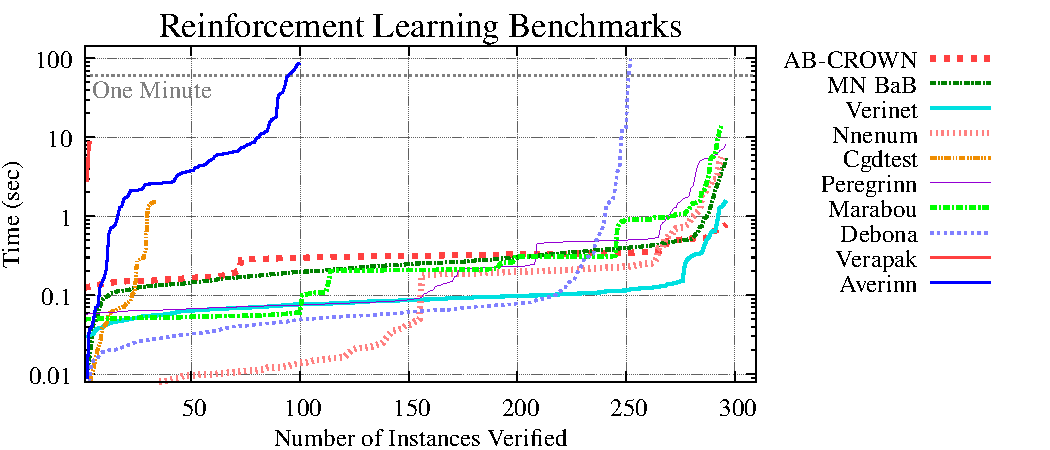
\includegraphics[width=\textwidth]{cactus/rl_benchmarks.pdf}}
\caption{Cactus Plot for Reinforcement Learning Benchmarks.}
\label{fig:quantPic}
\end{figure}


% Category sri_resnet_a (single_overhead=True):

\begin{table}[h]
\begin{center}
\caption{Benchmark \texttt{sri-resnet-a}} \label{tab:cat_{cat}}
{\setlength{\tabcolsep}{2pt}
\begin{tabular}[h]{@{}llllllrr@{}}
\toprule
\textbf{\# ~} & \textbf{Tool} & \textbf{Verified} & \textbf{Falsified} & \textbf{Fastest} & \textbf{Penalty} & \textbf{Score} & \textbf{Percent}\\
\midrule
1 & $\alpha$,$\beta$ Crown & 20 & 12 & 7 & 0 & 356 & 100.0\% \\
2 & Cgdtest & 26 & 6 & 14 & 0 & 352 & 98.9\% \\
3 & MN BaB & 18 & 12 & 19 & 0 & 343 & 96.3\% \\
4 & Verinet & 12 & 12 & 4 & 0 & 248 & 69.7\% \\
\bottomrule
\end{tabular}
}
\end{center}
\end{table}



\begin{figure}[h]
\centerline{\includegraphics[width=\textwidth]{cactus/sri_resnet_a.pdf}}
\caption{Cactus Plot for SRI Resnet A.}
\label{fig:quantPic}
\end{figure}


% Category sri_resnet_b (single_overhead=True):

\begin{table}[h]
\begin{center}
\caption{Benchmark \texttt{sri-resnet-b}} \label{tab:cat_{cat}}
{\setlength{\tabcolsep}{2pt}
\begin{tabular}[h]{@{}llllllrr@{}}
\toprule
\textbf{\# ~} & \textbf{Tool} & \textbf{Verified} & \textbf{Falsified} & \textbf{Fastest} & \textbf{Penalty} & \textbf{Score} & \textbf{Percent}\\
\midrule
1 & MN BaB & 27 & 11 & 24 & 0 & 435 & 100.0\% \\
2 & $\alpha$,$\beta$ Crown & 28 & 11 & 9 & 0 & 435 & 100.0\% \\
3 & Cgdtest & 22 & 10 & 9 & 0 & 340 & 78.2\% \\
4 & Verinet & 20 & 11 & 4 & 0 & 321 & 73.8\% \\
\bottomrule
\end{tabular}
}
\end{center}
\end{table}



\begin{figure}[h]
\centerline{\includegraphics[width=\textwidth]{cactus/sri_resnet_b.pdf}}
\caption{Cactus Plot for SRI Resnet B.}
\label{fig:quantPic}
\end{figure}


% Category tllverifybench (single_overhead=True):

\begin{table}[h]
\begin{center}
\caption{Benchmark \texttt{tllverifybench}} \label{tab:cat_{cat}}
{\setlength{\tabcolsep}{2pt}
\begin{tabular}[h]{@{}llllllrr@{}}
\toprule
\textbf{\# ~} & \textbf{Tool} & \textbf{Verified} & \textbf{Falsified} & \textbf{Fastest} & \textbf{Penalty} & \textbf{Score} & \textbf{Percent}\\
\midrule
1 & Fastbatllnn & 11 & 21 & 32 & 0 & 384 & 100.0\% \\
2 & MN BaB & 11 & 21 & 21 & 0 & 364 & 94.8\% \\
3 & $\alpha$,$\beta$ Crown & 11 & 21 & 12 & 0 & 353 & 91.9\% \\
4 & Peregrinn & 10 & 21 & 7 & 0 & 324 & 84.4\% \\
5 & Verinet & 11 & 21 & 0 & 0 & 320 & 83.3\% \\
6 & Nnenum & 1 & 21 & 10 & 0 & 240 & 62.5\% \\
7 & Debona & 0 & 19 & 10 & 0 & 210 & 54.7\% \\
8 & Marabou & 4 & 15 & 2 & 0 & 194 & 50.5\% \\
9 & Cgdtest & 0 & 9 & 6 & 1 & 2 & 0.5\% \\
\bottomrule
\end{tabular}
}
\end{center}
\end{table}



\begin{figure}[h]
\centerline{\includegraphics[width=\textwidth]{cactus/tllverifybench.pdf}}
\caption{Cactus Plot for Two-Level Lattice Verify Benchmark.}
\label{fig:quantPic}
\end{figure}


% Category vggnet16_2022 (single_overhead=True):

\begin{table}[h]
\begin{center}
\caption{Benchmark \texttt{vggnet16-2022}} \label{tab:cat_{cat}}
{\setlength{\tabcolsep}{2pt}
\begin{tabular}[h]{@{}llllllrr@{}}
\toprule
\textbf{\# ~} & \textbf{Tool} & \textbf{Verified} & \textbf{Falsified} & \textbf{Fastest} & \textbf{Penalty} & \textbf{Score} & \textbf{Percent}\\
\midrule
1 & $\alpha$,$\beta$ Crown & 14 & 1 & 11 & 0 & 176 & 100.0\% \\
2 & Nnenum & 11 & 1 & 0 & 0 & 127 & 72.2\% \\
3 & MN BaB & 5 & 1 & 4 & 0 & 69 & 39.2\% \\
4 & Verinet & 5 & 1 & 0 & 0 & 60 & 34.1\% \\
5 & Cgdtest & 0 & 2 & 1 & 4 & -378 & 0\% \\
\bottomrule
\end{tabular}
}
\end{center}
\end{table}



\begin{figure}[h]
\centerline{\includegraphics[width=\textwidth]{cactus/vggnet16_2022.pdf}}
\caption{Cactus Plot for VGGNet16 2022.}
\label{fig:quantPic}
\end{figure}



\clearpage
\section{Unscored Benchmarks}

% Category acasxu (single_overhead=True):

\begin{table}[h]
\begin{center}
\caption{Benchmark \texttt{acasxu}} \label{tab:cat_{cat}}
{\setlength{\tabcolsep}{2pt}
\begin{tabular}[h]{@{}llllllrr@{}}
\toprule
\textbf{\# ~} & \textbf{Tool} & \textbf{Verified} & \textbf{Falsified} & \textbf{Fastest} & \textbf{Penalty} & \textbf{Score} & \textbf{Percent}\\
\midrule
1 & Nnenum & 139 & 47 & 174 & 0 & 2218 & 100.0\% \\
2 & $\alpha$,$\beta$-CROWN & 139 & 46 & 59 & 0 & 2021 & 91.1\% \\
3 & MN BaB & 110 & 46 & 52 & 0 & 1664 & 75.0\% \\
4 & Cgdtest & 85 & 30 & 115 & 7 & 680 & 30.7\% \\
\bottomrule
\end{tabular}
}
\end{center}
\end{table}



% Category cifar2020 (single_overhead=True):

\begin{table}[h]
\begin{center}
\caption{Benchmark \texttt{cifar2020}} \label{tab:cat_{cat}}
{\setlength{\tabcolsep}{2pt}
\begin{tabular}[h]{@{}llllllrr@{}}
\toprule
\textbf{\# ~} & \textbf{Tool} & \textbf{Verified} & \textbf{Falsified} & \textbf{Fastest} & \textbf{Penalty} & \textbf{Score} & \textbf{Percent}\\
\midrule
1 & Verinet & 91 & 35 & 109 & 0 & 1486 & 100.0\% \\
2 & $\alpha$,$\beta$-CROWN & 95 & 34 & 78 & 0 & 1479 & 99.5\% \\
3 & MN BaB & 93 & 28 & 26 & 0 & 1275 & 85.8\% \\
4 & Nnenum & 66 & 19 & 0 & 0 & 850 & 57.2\% \\
5 & Cgdtest & 63 & 26 & 5 & 6 & 305 & 20.5\% \\
6 & Verapak & 0 & 15 & 1 & 0 & 152 & 10.2\% \\
7 & Marabou & 4 & 0 & 0 & 1 & -60 & 0\% \\
\bottomrule
\end{tabular}
}
\end{center}
\end{table}




\clearpage
\section{Stats}

%%%%%%%%%% Stats %%%%%%%%%%%

% Overhead:

\begin{table}[h]
\begin{center}
\caption{Overhead} \label{tab:overhead}
{\setlength{\tabcolsep}{2pt}
\begin{tabular}[h]{@{}llr@{}}
\toprule
\textbf{\# ~} & \textbf{Tool} & \textbf{Seconds}\\
\midrule
1 & Marabou & 0.2 \\
2 & Fastbatllnn & 0.5 \\
3 & Nnenum & 0.9 \\
4 & Cgdtest & 1.3 \\
5 & Peregrinn & 1.3 \\
6 & Debona & 2.0 \\
7 & Averinn & 3.1 \\
8 & Verinet & 3.4 \\
9 & Verapak & 4.6 \\
10 & $\alpha$,$\beta$ Crown & 6.7 \\
11 & MN BaB & 8.2 \\
\bottomrule
\end{tabular}
}
\end{center}
\end{table}



% Num Benchmarks Participated:

\begin{table}[h]
\begin{center}
\caption{Num Benchmarks Participated} \label{tab:stats0}
{\setlength{\tabcolsep}{2pt}
\begin{tabular}[h]{@{}llr@{}}
\toprule
\textbf{\# ~} & \textbf{Tool} & \textbf{Count}\\
\midrule
1 & Verinet & 13 \\
2 & MN BaB & 13 \\
3 & $\alpha$,$\beta$ Crown & 13 \\
4 & Cgdtest & 12 \\
5 & Nnenum & 9 \\
6 & Peregrinn & 7 \\
7 & Marabou & 6 \\
8 & Debona & 5 \\
9 & Verapak & 3 \\
10 & Fastbatllnn & 1 \\
11 & Averinn & 1 \\
\bottomrule
\end{tabular}
}
\end{center}
\end{table}



% Num Instances Verified:

\begin{table}[h]
\begin{center}
\caption{Num Instances Verified} \label{tab:stats1}
{\setlength{\tabcolsep}{2pt}
\begin{tabular}[h]{@{}llr@{}}
\toprule
\textbf{\# ~} & \textbf{Tool} & \textbf{Count}\\
\midrule
1 & $\alpha$,$\beta$ Crown & 950 \\
2 & MN BaB & 812 \\
3 & Verinet & 754 \\
4 & Nnenum & 515 \\
5 & Peregrinn & 478 \\
6 & Marabou & 450 \\
7 & Cgdtest & 405 \\
8 & Debona & 341 \\
9 & Verapak & 117 \\
10 & Averinn & 100 \\
11 & Fastbatllnn & 32 \\
\bottomrule
\end{tabular}
}
\end{center}
\end{table}



% Num SAT:

\begin{table}[h]
\begin{center}
\caption{Num SAT} \label{tab:stats2}
{\setlength{\tabcolsep}{2pt}
\begin{tabular}[h]{@{}llr@{}}
\toprule
\textbf{\# ~} & \textbf{Tool} & \textbf{Count}\\
\midrule
1 & Verinet & 228 \\
2 & MN BaB & 227 \\
3 & $\alpha$,$\beta$ Crown & 227 \\
4 & Nnenum & 196 \\
5 & Peregrinn & 191 \\
6 & Marabou & 148 \\
7 & Debona & 138 \\
8 & Cgdtest & 101 \\
9 & Fastbatllnn & 21 \\
10 & Averinn & 8 \\
11 & Verapak & 6 \\
\bottomrule
\end{tabular}
}
\end{center}
\end{table}



% Num UNSAT:

\begin{table}[h]
\begin{center}
\caption{Num UNSAT} \label{tab:stats3}
{\setlength{\tabcolsep}{2pt}
\begin{tabular}[h]{@{}llr@{}}
\toprule
\textbf{\# ~} & \textbf{Tool} & \textbf{Count}\\
\midrule
1 & $\alpha$,$\beta$ Crown & 723 \\
2 & MN BaB & 585 \\
3 & Verinet & 526 \\
4 & Nnenum & 319 \\
5 & Cgdtest & 304 \\
6 & Marabou & 302 \\
7 & Peregrinn & 287 \\
8 & Debona & 203 \\
9 & Verapak & 111 \\
10 & Averinn & 92 \\
11 & Fastbatllnn & 11 \\
\bottomrule
\end{tabular}
}
\end{center}
\end{table}



% Incorrect Results (or Missing CE):

\begin{table}[h]
\begin{center}
\caption{Incorrect Results (or Missing CE)} \label{tab:stats4}
{\setlength{\tabcolsep}{2pt}
\begin{tabular}[h]{@{}llr@{}}
\toprule
\textbf{\# ~} & \textbf{Tool} & \textbf{Count}\\
\midrule
1 & Cgdtest & 41 \\
2 & Verapak & 5 \\
3 & Marabou & 1 \\
4 & $\alpha$,$\beta$ Crown & 1 \\
\bottomrule
\end{tabular}
}
\end{center}
\end{table}




\clearpage
\section{Detailed Results}
% Long table of all results


\begin{center}
{\setlength{\tabcolsep}{1pt}
\scriptsize
\begin{longtable}{@{}llllllllllllll@{}}
\caption{\footnotesize Tools: $\alpha$,$\beta$ Crown (T1), MN BaB (T2), Verinet (T3), Nnenum (T4), Cgdtest (T5), Peregrinn (T6), Marabou (T7), Debona (T8), Fastbatllnn (T9), Verapak (T10), Averinn (T11)} \label{tab:all_results} \\
\toprule
\textbf{Category} & \textbf{Id} & \textbf{Result} & \textbf{$\alpha$,$\beta$-C} & \textbf{MnB} & \textbf{Verin} & \textbf{nnen} & \textbf{CGD} & \textbf{Pereg} & \textbf{Marab} & \textbf{Debon} & \textbf{FastBaT} & \textbf{Verap} & \textbf{Averi} \\
\midrule
\endhead
carvana 2022 & 0 & \textsc{unsat} & \textcolor{blue}{7.5} & - & - & - & - & - & - & - & - & - & - \\
carvana 2022 & 1 & \textsc{unsat} & \textcolor{blue}{26.1} & \textcolor{black}{76.4} & - & - & - & - & - & - & - & - & - \\
carvana 2022 & 2 & - & - & - & - & - & - & - & - & - & - & - & - \\
carvana 2022 & 3 & - & - & - & - & - & - & - & - & - & - & - & - \\
carvana 2022 & 4 & \textsc{unsat} & \textcolor{blue}{7.8} & - & - & - & - & - & - & - & - & - & - \\
carvana 2022 & 5 & \textsc{unsat} & \textcolor{blue}{8.7} & - & - & - & - & - & - & - & - & - & - \\
carvana 2022 & 6 & \textsc{unsat} & \textcolor{blue}{26.9} & - & - & - & - & - & - & - & - & - & - \\
carvana 2022 & 7 & - & - & - & - & - & - & - & - & - & - & - & - \\
carvana 2022 & 8 & - & - & - & - & - & - & - & - & - & - & - & - \\
carvana 2022 & 9 & \textsc{unsat} & \textcolor{blue}{26.2} & \textcolor{black}{148} & - & - & - & - & - & - & - & - & - \\
carvana 2022 & 10 & - & - & - & - & - & - & - & - & - & - & - & - \\
carvana 2022 & 11 & \textsc{unsat} & \textcolor{blue}{26.2} & \textcolor{black}{39.1} & - & - & - & - & - & - & - & - & - \\
carvana 2022 & 12 & \textsc{unsat} & \textcolor{blue}{26.9} & - & - & - & - & - & - & - & - & - & - \\
carvana 2022 & 13 & \textsc{unsat} & \textcolor{blue}{31.2} & \textcolor{black}{44.7} & - & - & - & - & - & - & - & - & - \\
carvana 2022 & 14 & - & - & - & - & - & - & - & - & - & - & - & - \\
carvana 2022 & 15 & - & - & - & - & - & - & - & - & - & - & - & - \\
carvana 2022 & 16 & \textsc{unsat} & \textcolor{blue}{7.0} & - & - & - & - & - & - & - & - & - & - \\
carvana 2022 & 17 & - & - & - & - & - & - & - & - & - & - & - & - \\
carvana 2022 & 18 & \textsc{unsat} & \textcolor{blue}{7.6} & - & - & - & - & - & - & - & - & - & - \\
carvana 2022 & 19 & \textsc{unsat} & \textcolor{blue}{7.0} & - & - & - & - & - & - & - & - & - & - \\
carvana 2022 & 20 & \textsc{unsat} & \textcolor{blue}{28.4} & \textcolor{black}{67.1} & - & - & - & - & - & - & - & - & - \\
carvana 2022 & 21 & - & - & - & - & - & - & - & - & - & - & - & - \\
carvana 2022 & 22 & \textsc{unsat} & \textcolor{blue}{6.1} & - & - & - & - & - & - & - & - & - & - \\
carvana 2022 & 23 & - & - & - & - & - & - & - & - & - & - & - & - \\
carvana 2022 & 24 & - & - & - & - & - & - & - & - & - & - & - & - \\
carvana 2022 & 25 & \textsc{unsat} & \textcolor{blue}{26.2} & \textcolor{black}{39.2} & - & - & - & - & - & - & - & - & - \\
carvana 2022 & 26 & - & - & - & - & - & - & - & - & - & - & - & - \\
carvana 2022 & 27 & - & - & - & - & - & - & - & - & - & - & - & - \\
carvana 2022 & 28 & - & - & - & - & - & - & - & - & - & - & - & - \\
carvana 2022 & 29 & - & - & - & - & - & - & - & - & - & - & - & - \\
carvana 2022 & 30 & \textsc{unsat} & \textcolor{blue}{26.8} & \textcolor{black}{132} & - & - & - & - & - & - & - & - & - \\
carvana 2022 & 31 & - & - & - & - & - & - & - & - & - & - & - & - \\
carvana 2022 & 32 & - & - & - & - & - & - & - & - & - & - & - & - \\
carvana 2022 & 33 & - & - & - & - & - & - & - & - & - & - & - & - \\
carvana 2022 & 34 & - & - & - & - & - & - & - & - & - & - & - & - \\
carvana 2022 & 35 & - & - & - & - & - & - & - & - & - & - & - & - \\
carvana 2022 & 36 & \textsc{unsat} & \textcolor{blue}{26.2} & \textcolor{black}{45.6} & - & - & - & - & - & - & - & - & - \\
carvana 2022 & 37 & \textsc{unsat} & \textcolor{blue}{7.0} & - & - & - & - & - & - & - & - & - & - \\
carvana 2022 & 38 & \textsc{unsat} & \textcolor{blue}{2.3} & \textcolor{black}{28.0} & \textcolor{darkgray}{264} & - & - & - & - & - & - & - & - \\
carvana 2022 & 39 & \textsc{unsat} & \textcolor{blue}{26.4} & \textcolor{black}{84.6} & - & - & - & - & - & - & - & - & - \\
carvana 2022 & 40 & \textsc{unsat} & \textcolor{blue}{26.3} & \textcolor{black}{61.6} & - & - & - & - & - & - & - & - & - \\
carvana 2022 & 41 & - & - & - & - & - & - & - & - & - & - & - & - \\
carvana 2022 & 42 & - & - & - & - & - & - & - & - & - & - & - & - \\
carvana 2022 & 43 & \textsc{unsat} & \textcolor{blue}{7.6} & - & - & - & - & - & - & - & - & - & - \\
carvana 2022 & 44 & \textsc{unsat} & \textcolor{blue}{7.5} & - & - & - & - & - & - & - & - & - & - \\
carvana 2022 & 45 & - & - & - & - & - & - & - & - & - & - & - & - \\
carvana 2022 & 46 & \textsc{unsat} & \textcolor{blue}{8.7} & - & - & - & - & - & - & - & - & - & - \\
carvana 2022 & 47 & - & - & - & - & - & - & - & - & - & - & - & - \\
carvana 2022 & 48 & - & - & - & - & - & - & - & - & - & - & - & - \\
carvana 2022 & 49 & \textsc{unsat} & \textcolor{blue}{26.1} & \textcolor{black}{52.9} & - & - & - & - & - & - & - & - & - \\
carvana 2022 & 50 & - & - & - & - & - & - & - & - & - & - & - & - \\
carvana 2022 & 51 & \textsc{unsat} & \textcolor{blue}{26.1} & \textcolor{black}{62.6} & - & - & - & - & - & - & - & - & - \\
carvana 2022 & 52 & \textsc{unsat} & \textcolor{blue}{8.6} & - & - & - & - & - & - & - & - & - & - \\
carvana 2022 & 53 & \textsc{unsat} & \textcolor{blue}{26.8} & - & - & - & - & - & - & - & - & - & - \\
carvana 2022 & 54 & - & - & - & - & - & - & - & - & - & - & - & - \\
carvana 2022 & 55 & \textsc{unsat} & \textcolor{blue}{26.9} & \textcolor{black}{170} & - & - & - & - & - & - & - & - & - \\
carvana 2022 & 56 & - & - & - & - & - & - & - & - & - & - & - & - \\
carvana 2022 & 57 & - & - & - & - & - & - & - & - & - & - & - & - \\
carvana 2022 & 58 & - & - & - & - & - & - & - & - & - & - & - & - \\
carvana 2022 & 59 & \textsc{unsat} & \textcolor{blue}{7.8} & - & - & - & - & - & - & - & - & - & - \\
carvana 2022 & 60 & \textsc{unsat} & \textcolor{blue}{26.1} & \textcolor{black}{40.8} & \textcolor{darkgray}{272} & - & - & - & - & - & - & - & - \\
carvana 2022 & 61 & \textsc{unsat} & \textcolor{blue}{31.2} & \textcolor{black}{78.6} & - & - & - & - & - & - & - & - & - \\
carvana 2022 & 62 & \textsc{unsat} & \textcolor{blue}{26.2} & \textcolor{black}{52.9} & - & - & - & - & - & - & - & - & - \\
carvana 2022 & 63 & \textsc{unsat} & \textcolor{blue}{7.7} & - & - & - & - & - & - & - & - & - & - \\
carvana 2022 & 64 & \textsc{unsat} & \textcolor{blue}{26.2} & \textcolor{black}{171} & - & - & - & - & - & - & - & - & - \\
carvana 2022 & 65 & - & - & - & - & - & - & - & - & - & - & - & - \\
carvana 2022 & 66 & - & - & - & - & - & - & - & - & - & - & - & - \\
carvana 2022 & 67 & \textsc{unsat} & \textcolor{blue}{25.9} & \textcolor{black}{31.8} & \textcolor{darkgray}{257} & - & - & - & - & - & - & - & - \\
carvana 2022 & 68 & \textsc{unsat} & \textcolor{blue}{6.2} & - & - & - & - & - & - & - & - & - & - \\
carvana 2022 & 69 & \textsc{unsat} & \textcolor{blue}{8.7} & - & - & - & - & - & - & - & - & - & - \\
carvana 2022 & 70 & - & - & - & - & - & - & - & - & - & - & - & - \\
carvana 2022 & 71 & \textsc{unsat} & \textcolor{blue}{8.5} & - & - & - & - & - & - & - & - & - & - \\
cifar100 tiny & 0 & \textsc{unsat} & \textcolor{blue}{8.9} & \textcolor{darkgray}{30.4} & \textcolor{black}{12.8} & - & \textcolor{darkgray}{32.7} & - & - & - & - & - & - \\
cifar100 tiny & 1 & \textsc{unsat} & \textcolor{blue}{12.9} & \textcolor{darkgray}{64.1} & - & - & \textcolor{black}{32.3} & - & - & - & - & - & - \\
cifar100 tiny & 2 & \textsc{unsat} & - & - & - & - & \textcolor{blue}{32.7} & - & - & - & - & - & - \\
cifar100 tiny & 3 & \textsc{unsat} & \textcolor{blue}{13.2} & \textcolor{darkgray}{52.1} & - & - & \textcolor{black}{31.7} & - & - & - & - & - & - \\
cifar100 tiny & 4 & \textsc{unsat} & - & - & - & - & \textcolor{blue}{31.8} & - & - & - & - & - & - \\
cifar100 tiny & 5 & \textsc{unsat} & - & - & - & - & \textcolor{blue}{32.9} & - & - & - & - & - & - \\
cifar100 tiny & 6 & \textsc{unsat} & - & - & - & - & \textcolor{blue}{32.3} & - & - & - & - & - & - \\
cifar100 tiny & 7 & \textsc{unsat} & \textcolor{blue}{13.0} & \textcolor{darkgray}{51.1} & - & - & \textcolor{black}{34.5} & - & - & - & - & - & - \\
cifar100 tiny & 8 & \textsc{unsat} & \textcolor{blue}{26.1} & - & - & - & \textcolor{black}{34.3} & - & - & - & - & - & - \\
cifar100 tiny & 9 & \textsc{unsat} & - & - & - & - & \textcolor{blue}{32.9} & - & - & - & - & - & - \\
cifar100 tiny & 10 & \textsc{unsat} & - & - & - & - & \textcolor{blue}{38.4} & - & - & - & - & - & - \\
cifar100 tiny & 11 & \textsc{unsat} & - & - & - & - & \textcolor{blue}{34.2} & - & - & - & - & - & - \\
cifar100 tiny & 12 & \textsc{unsat} & - & - & - & - & \textcolor{blue}{35.4} & - & - & - & - & - & - \\
cifar100 tiny & 13 & \textsc{unsat} & \textcolor{blue}{9.8} & \textcolor{black}{31.4} & \textcolor{darkgray}{65.4} & - & \textcolor{darkgray}{35.9} & - & - & - & - & - & - \\
cifar100 tiny & 14 & \textsc{unsat} & \textcolor{blue}{9.0} & \textcolor{darkgray}{29.1} & \textcolor{black}{12.7} & - & \textcolor{darkgray}{37.1} & - & - & - & - & - & - \\
cifar100 tiny & 15 & \textsc{unsat} & \textcolor{blue}{9.6} & \textcolor{darkgray}{31.0} & \textcolor{black}{22.0} & - & \textcolor{darkgray}{34.5} & - & - & - & - & - & - \\
cifar100 tiny & 16 & \textsc{unsat} & \textcolor{blue}{9.2} & \textcolor{darkgray}{23.0} & \textcolor{black}{14.6} & - & \textcolor{darkgray}{35.0} & - & - & - & - & - & - \\
cifar100 tiny & 17 & \textsc{unsat} & \textcolor{blue}{14.7} & \textcolor{darkgray}{138} & - & - & \textcolor{black}{35.4} & - & - & - & - & - & - \\
cifar100 tiny & 18 & \textsc{unsat} & \textcolor{blue}{9.1} & \textcolor{darkgray}{27.6} & \textcolor{black}{19.9} & - & \textcolor{darkgray}{35.0} & - & - & - & - & - & - \\
cifar100 tiny & 19 & \textsc{unsat} & \textcolor{blue}{24.7} & - & - & - & \textcolor{black}{36.5} & - & - & - & - & - & - \\
cifar100 tiny & 20 & \textsc{unsat} & \textcolor{blue}{9.3} & \textcolor{darkgray}{19.8} & \textcolor{black}{15.9} & - & \textcolor{darkgray}{35.5} & - & - & - & - & - & - \\
cifar100 tiny & 21 & \textsc{unsat} & \textcolor{blue}{12.1} & \textcolor{darkgray}{81.5} & - & - & \textcolor{black}{35.0} & - & - & - & - & - & - \\
cifar100 tiny & 22 & \textsc{unsat} & \textcolor{blue}{10.0} & \textcolor{darkgray}{52.2} & \textcolor{darkgray}{73.1} & - & \textcolor{black}{35.3} & - & - & - & - & - & - \\
cifar100 tiny & 23 & \textsc{unsat} & \textcolor{blue}{10.4} & \textcolor{darkgray}{45.5} & \textcolor{darkgray}{100} & - & \textcolor{black}{35.4} & - & - & - & - & - & - \\
cifar100 tiny & 24 & \textsc{unsat} & - & - & - & - & \textcolor{blue}{35.5} & - & - & - & - & - & - \\
cifar100 tiny & 25 & \textsc{unsat} & \textcolor{black}{9.1} & \textcolor{darkgray}{23.3} & \textcolor{blue}{8.6} & - & \textcolor{darkgray}{36.6} & - & - & - & - & - & - \\
cifar100 tiny & 26 & \textsc{unsat} & \textcolor{blue}{11.7} & \textcolor{darkgray}{69.1} & - & - & \textcolor{black}{36.0} & - & - & - & - & - & - \\
cifar100 tiny & 27 & \textsc{unsat} & - & - & - & - & \textcolor{blue}{36.5} & - & - & - & - & - & - \\
cifar100 tiny & 28 & \textsc{unsat} & \textcolor{blue}{9.9} & \textcolor{black}{35.0} & \textcolor{darkgray}{50.6} & - & \textcolor{darkgray}{35.2} & - & - & - & - & - & - \\
cifar100 tiny & 29 & \textsc{unsat} & \textcolor{blue}{10.0} & \textcolor{darkgray}{37.4} & \textcolor{darkgray}{54.0} & - & \textcolor{black}{36.5} & - & - & - & - & - & - \\
cifar100 tiny & 30 & \textsc{unsat} & \textcolor{black}{6.2} & \textcolor{darkgray}{8.1} & \textcolor{blue}{4.0} & - & \textcolor{darkgray}{37.4} & - & - & - & - & - & - \\
cifar100 tiny & 31 & \textsc{unsat} & \textcolor{blue}{13.9} & \textcolor{darkgray}{173} & - & - & \textcolor{black}{35.1} & - & - & - & - & - & - \\
cifar100 tiny & 32 & \textsc{unsat} & \textcolor{blue}{9.0} & \textcolor{darkgray}{25.7} & \textcolor{black}{20.2} & - & \textcolor{darkgray}{38.7} & - & - & - & - & - & - \\
cifar100 tiny & 33 & \textsc{unsat} & \textcolor{blue}{10.1} & \textcolor{darkgray}{35.5} & \textcolor{darkgray}{71.1} & - & \textcolor{black}{35.2} & - & - & - & - & - & - \\
cifar100 tiny & 34 & \textsc{unsat} & \textcolor{blue}{11.8} & \textcolor{black}{14.6} & \textcolor{darkgray}{15.7} & - & \textcolor{darkgray}{47.7} & - & - & - & - & - & - \\
cifar100 tiny & 35 & \textsc{unsat} & \textcolor{black}{53.4} & - & - & - & \textcolor{blue}{48.8} & - & - & - & - & - & - \\
cifar100 tiny & 36 & \textsc{unsat} & \textcolor{blue}{12.3} & \textcolor{blue}{12.4} & \textcolor{darkgray}{13.2} & - & \textcolor{darkgray}{48.5} & - & - & - & - & - & - \\
cifar100 tiny & 37 & \textsc{unsat} & \textcolor{darkgray}{13.1} & \textcolor{blue}{11.7} & \textcolor{black}{12.8} & - & \textcolor{darkgray}{47.8} & - & - & - & - & - & - \\
cifar100 tiny & 38 & \textsc{unsat} & \textcolor{blue}{27.5} & - & - & - & \textcolor{black}{49.3} & - & - & - & - & - & - \\
cifar100 tiny & 39 & \textsc{unsat} & \textcolor{black}{4.9} & \textcolor{darkgray}{6.6} & \textcolor{blue}{4.6} & - & \textcolor{darkgray}{48.2} & - & - & - & - & - & - \\
cifar100 tiny & 40 & \textsc{unsat} & \textcolor{blue}{12.7} & \textcolor{black}{24.8} & \textcolor{darkgray}{128} & - & \textcolor{darkgray}{48.2} & - & - & - & - & - & - \\
cifar100 tiny & 41 & \textsc{unsat} & \textcolor{blue}{13.1} & \textcolor{black}{43.7} & - & - & \textcolor{darkgray}{49.4} & - & - & - & - & - & - \\
cifar100 tiny & 42 & \textsc{unsat} & \textcolor{blue}{11.1} & \textcolor{darkgray}{16.3} & \textcolor{black}{12.9} & - & \textcolor{darkgray}{48.2} & - & - & - & - & - & - \\
cifar100 tiny & 43 & \textsc{unsat} & \textcolor{blue}{4.6} & \textcolor{darkgray}{6.7} & \textcolor{blue}{4.7} & - & \textcolor{darkgray}{48.6} & - & - & - & - & - & - \\
cifar100 tiny & 44 & \textsc{unsat} & - & - & - & - & \textcolor{blue}{49.5} & - & - & - & - & - & - \\
cifar100 tiny & 45 & \textsc{unsat} & \textcolor{blue}{12.2} & \textcolor{black}{19.6} & \textcolor{darkgray}{30.0} & - & \textcolor{darkgray}{47.7} & - & - & - & - & - & - \\
cifar100 tiny & 46 & \textsc{unsat} & \textcolor{blue}{38.8} & - & - & - & \textcolor{black}{50.3} & - & - & - & - & - & - \\
cifar100 tiny & 47 & \textsc{unsat} & \textcolor{blue}{13.8} & \textcolor{darkgray}{76.9} & - & - & \textcolor{black}{48.1} & - & - & - & - & - & - \\
cifar100 tiny & 48 & \textsc{unsat} & - & - & - & - & \textcolor{blue}{48.4} & - & - & - & - & - & - \\
cifar100 tiny & 49 & \textsc{unsat} & \textcolor{blue}{11.7} & \textcolor{darkgray}{22.1} & \textcolor{black}{14.2} & - & \textcolor{darkgray}{49.2} & - & - & - & - & - & - \\
cifar100 tiny & 50 & \textsc{unsat} & \textcolor{black}{6.6} & \textcolor{black}{6.7} & \textcolor{blue}{4.8} & - & \textcolor{darkgray}{48.2} & - & - & - & - & - & - \\
cifar100 tiny & 51 & \textsc{unsat} & \textcolor{blue}{12.0} & \textcolor{black}{14.1} & \textcolor{darkgray}{18.7} & - & \textcolor{darkgray}{48.1} & - & - & - & - & - & - \\
cifar100 tiny & 52 & \textsc{unsat} & - & - & - & - & \textcolor{blue}{48.7} & - & - & - & - & - & - \\
cifar100 tiny & 53 & \textsc{unsat} & \textcolor{blue}{10.6} & \textcolor{darkgray}{20.1} & \textcolor{black}{17.7} & - & \textcolor{darkgray}{48.1} & - & - & - & - & - & - \\
cifar100 tiny & 54 & \textsc{unsat} & \textcolor{blue}{11.6} & \textcolor{black}{26.5} & \textcolor{darkgray}{192} & - & \textcolor{darkgray}{49.2} & - & - & - & - & - & - \\
cifar100 tiny & 55 & \textsc{unsat} & \textcolor{black}{10.7} & \textcolor{blue}{8.7} & \textcolor{darkgray}{10.9} & - & \textcolor{darkgray}{50.9} & - & - & - & - & - & - \\
cifar100 tiny & 56 & \textsc{unsat} & \textcolor{black}{11.3} & \textcolor{blue}{11.0} & \textcolor{darkgray}{12.2} & - & \textcolor{darkgray}{47.9} & - & - & - & - & - & - \\
cifar100 tiny & 57 & \textsc{unsat} & \textcolor{blue}{11.6} & \textcolor{black}{22.3} & \textcolor{darkgray}{86.6} & - & \textcolor{darkgray}{48.4} & - & - & - & - & - & - \\
cifar100 tiny & 58 & \textsc{unsat} & \textcolor{blue}{9.6} & \textcolor{black}{24.1} & \textcolor{darkgray}{25.5} & - & \textcolor{darkgray}{38.1} & - & - & - & - & - & - \\
cifar100 tiny & 59 & \textsc{unsat} & \textcolor{blue}{9.7} & \textcolor{black}{14.0} & \textcolor{darkgray}{14.5} & - & \textcolor{darkgray}{38.4} & - & - & - & - & - & - \\
cifar100 tiny & 60 & \textsc{unsat} & - & - & - & - & \textcolor{blue}{37.9} & - & - & - & - & - & - \\
cifar100 tiny & 61 & \textsc{unsat} & - & - & - & - & \textcolor{blue}{38.3} & - & - & - & - & - & - \\
cifar100 tiny & 62 & \textsc{unsat} & - & - & - & - & \textcolor{blue}{38.3} & - & - & - & - & - & - \\
cifar100 tiny & 63 & \textsc{unsat} & \textcolor{blue}{10.9} & \textcolor{black}{36.3} & \textcolor{darkgray}{115} & - & \textcolor{darkgray}{38.3} & - & - & - & - & - & - \\
cifar100 tiny & 64 & \textsc{unsat} & \textcolor{blue}{10.0} & \textcolor{darkgray}{14.3} & \textcolor{black}{13.1} & - & \textcolor{darkgray}{40.6} & - & - & - & - & - & - \\
cifar100 tiny & 65 & \textsc{unsat} & \textcolor{blue}{10.2} & \textcolor{black}{28.6} & \textcolor{darkgray}{59.7} & - & \textcolor{darkgray}{38.5} & - & - & - & - & - & - \\
cifar100 tiny & 66 & \textsc{unsat} & - & - & - & - & \textcolor{blue}{38.1} & - & - & - & - & - & - \\
cifar100 tiny & 67 & \textsc{unsat} & \textcolor{blue}{9.7} & \textcolor{darkgray}{22.0} & \textcolor{black}{16.6} & - & \textcolor{darkgray}{38.6} & - & - & - & - & - & - \\
cifar100 tiny & 68 & \textsc{unsat} & \textcolor{black}{6.0} & \textcolor{darkgray}{6.5} & \textcolor{blue}{4.3} & - & \textcolor{darkgray}{38.2} & - & - & - & - & - & - \\
cifar100 tiny & 69 & \textsc{unsat} & - & - & - & - & \textcolor{blue}{41.0} & - & - & - & - & - & - \\
cifar100 tiny & 70 & \textsc{unsat} & - & - & - & - & \textcolor{blue}{38.6} & - & - & - & - & - & - \\
cifar100 tiny & 71 & \textsc{unsat} & \textcolor{black}{46.9} & - & - & - & \textcolor{blue}{38.7} & - & - & - & - & - & - \\
cifar100 tiny & 72 & \textsc{unsat} & \textcolor{blue}{11.1} & \textcolor{black}{32.4} & \textcolor{darkgray}{101} & - & \textcolor{darkgray}{37.8} & - & - & - & - & - & - \\
cifar100 tiny & 73 & \textsc{unsat} & - & - & - & - & \textcolor{blue}{40.0} & - & - & - & - & - & - \\
cifar100 tiny & 74 & \textsc{unsat} & - & - & - & - & \textcolor{blue}{109} & - & - & - & - & - & - \\
cifar100 tiny & 75 & \textsc{unsat} & \textcolor{black}{11.7} & \textcolor{blue}{7.3} & \textcolor{black}{11.5} & - & \textcolor{darkgray}{106} & - & - & - & - & - & - \\
cifar100 tiny & 76 & \textsc{unsat} & \textcolor{blue}{16.2} & \textcolor{black}{81.8} & - & - & \textcolor{darkgray}{106} & - & - & - & - & - & - \\
cifar100 tiny & 77 & \textsc{unsat} & \textcolor{blue}{16.9} & \textcolor{black}{62.9} & - & - & \textcolor{darkgray}{106} & - & - & - & - & - & - \\
cifar100 tiny & 78 & \textsc{unsat} & \textcolor{blue}{4.8} & \textcolor{black}{7.9} & \textcolor{darkgray}{12.3} & - & \textcolor{darkgray}{107} & - & - & - & - & - & - \\
cifar100 tiny & 79 & \textsc{unsat} & \textcolor{blue}{13.5} & \textcolor{black}{16.1} & \textcolor{darkgray}{53.1} & - & \textcolor{darkgray}{105} & - & - & - & - & - & - \\
cifar100 tiny & 80 & \textsc{unsat} & \textcolor{blue}{13.7} & \textcolor{black}{22.4} & \textcolor{darkgray}{76.8} & - & \textcolor{darkgray}{105} & - & - & - & - & - & - \\
cifar100 tiny & 81 & \textsc{unsat} & \textcolor{black}{12.9} & \textcolor{blue}{9.2} & \textcolor{darkgray}{13.5} & - & \textcolor{darkgray}{106} & - & - & - & - & - & - \\
cifar100 tiny & 82 & \textsc{sat} & - & \textcolor{blue}{1.5} & \textcolor{black}{5.4} & - & \textbf{\textcolor{red}{106}} & - & - & - & - & - & - \\
cifar100 tiny & 83 & \textsc{unsat} & \textcolor{blue}{14.4} & \textcolor{black}{29.3} & - & - & \textcolor{darkgray}{107} & - & - & - & - & - & - \\
cifar100 tiny & 84 & \textsc{sat} & - & \textcolor{blue}{1.2} & \textcolor{black}{4.7} & - & \textbf{\textcolor{red}{107}} & - & - & - & - & - & - \\
cifar100 tiny & 85 & \textsc{unsat} & - & - & - & - & \textcolor{blue}{109} & - & - & - & - & - & - \\
cifar100 tiny & 86 & \textsc{unsat} & \textcolor{blue}{12.8} & \textcolor{black}{21.3} & \textcolor{darkgray}{43.8} & - & \textcolor{darkgray}{106} & - & - & - & - & - & - \\
cifar100 tiny & 87 & \textsc{sat} & - & \textcolor{blue}{1.6} & \textcolor{black}{4.9} & - & \textbf{\textcolor{red}{106}} & - & - & - & - & - & - \\
cifar100 tiny & 88 & \textsc{unsat} & - & - & - & - & \textcolor{blue}{104} & - & - & - & - & - & - \\
cifar100 tiny & 89 & \textsc{unsat} & - & - & - & - & \textcolor{blue}{100} & - & - & - & - & - & - \\
cifar100 tiny & 90 & \textsc{unsat} & \textcolor{blue}{25.9} & - & - & - & \textcolor{black}{98.9} & - & - & - & - & - & - \\
cifar100 tiny & 91 & \textsc{unsat} & - & - & - & - & \textcolor{blue}{102} & - & - & - & - & - & - \\
cifar100 tiny & 92 & \textsc{unsat} & \textcolor{blue}{11.2} & \textcolor{black}{12.1} & \textcolor{darkgray}{15.8} & - & \textcolor{darkgray}{107} & - & - & - & - & - & - \\
cifar100 tiny & 93 & \textsc{unsat} & \textcolor{blue}{11.9} & \textcolor{black}{17.5} & \textcolor{darkgray}{18.1} & - & \textcolor{darkgray}{106} & - & - & - & - & - & - \\
cifar100 tiny & 94 & \textsc{unsat} & \textcolor{blue}{20.5} & - & - & - & \textcolor{black}{106} & - & - & - & - & - & - \\
cifar100 tiny & 95 & \textsc{unsat} & \textcolor{darkgray}{13.1} & \textcolor{blue}{10.5} & \textcolor{black}{11.8} & - & \textcolor{darkgray}{100.0} & - & - & - & - & - & - \\
cifar100 tiny & 96 & \textsc{unsat} & - & - & - & - & \textcolor{blue}{103} & - & - & - & - & - & - \\
cifar100 tiny & 97 & \textsc{unsat} & \textcolor{blue}{55.0} & - & - & - & \textcolor{black}{105} & - & - & - & - & - & - \\
cifar biasfield & 0 & \textsc{unsat} & \textcolor{darkgray}{4.9} & \textcolor{darkgray}{33.6} & \textcolor{black}{4.7} & - & \textcolor{blue}{3.2} & - & \textcolor{darkgray}{115} & - & - & \textcolor{darkgray}{5.2} & - \\
cifar biasfield & 1 & \textsc{unsat} & \textcolor{darkgray}{6.2} & - & \textcolor{darkgray}{5.5} & - & \textcolor{blue}{3.3} & - & \textcolor{darkgray}{114} & - & - & \textcolor{black}{5.0} & - \\
cifar biasfield & 2 & \textsc{unsat} & \textcolor{black}{4.0} & \textcolor{darkgray}{6.5} & \textcolor{darkgray}{4.5} & - & \textcolor{blue}{3.2} & - & \textcolor{darkgray}{115} & - & - & \textcolor{darkgray}{5.2} & - \\
cifar biasfield & 3 & \textsc{unsat} & \textcolor{darkgray}{6.3} & - & \textcolor{darkgray}{6.0} & - & \textcolor{blue}{3.7} & - & - & - & - & \textcolor{black}{5.1} & - \\
cifar biasfield & 4 & \textsc{unsat} & \textcolor{darkgray}{19.6} & - & \textcolor{darkgray}{16.8} & - & \textcolor{blue}{3.2} & - & - & - & - & \textcolor{black}{5.1} & - \\
cifar biasfield & 5 & \textsc{unsat} & \textcolor{darkgray}{5.6} & - & \textcolor{darkgray}{5.6} & - & \textcolor{blue}{3.4} & - & - & - & - & \textcolor{black}{5.1} & - \\
cifar biasfield & 6 & \textsc{unsat} & \textcolor{black}{3.4} & \textcolor{blue}{1.2} & \textcolor{darkgray}{3.9} & - & \textcolor{black}{3.3} & - & - & - & - & \textcolor{darkgray}{5.1} & - \\
cifar biasfield & 7 & \textsc{unsat} & \textcolor{darkgray}{8.2} & - & \textcolor{darkgray}{8.1} & - & \textcolor{blue}{3.6} & - & \textcolor{darkgray}{115} & - & - & \textcolor{black}{5.5} & - \\
cifar biasfield & 8 & \textsc{sat} & \textcolor{blue}{0.5} & \textcolor{blue}{1.2} & \textcolor{darkgray}{4.3} & - & \textbf{\textcolor{red}{3.6}} & - & - & - & - & \textbf{\textcolor{red}{14.6}} & - \\
cifar biasfield & 9 & \textsc{unsat} & \textcolor{darkgray}{6.1} & \textcolor{darkgray}{151} & \textcolor{black}{5.1} & - & \textcolor{blue}{3.1} & - & \textcolor{darkgray}{115} & - & - & \textcolor{darkgray}{12.8} & - \\
cifar biasfield & 10 & \textsc{unsat} & \textcolor{black}{9.0} & - & \textcolor{black}{8.8} & - & \textcolor{blue}{3.5} & - & - & - & - & \textcolor{darkgray}{12.4} & - \\
cifar biasfield & 11 & \textsc{unsat} & \textcolor{darkgray}{5.3} & - & \textcolor{black}{4.7} & - & \textcolor{blue}{3.3} & - & - & - & - & \textcolor{darkgray}{14.2} & - \\
cifar biasfield & 12 & \textsc{unsat} & \textcolor{darkgray}{150} & - & \textcolor{darkgray}{72.8} & - & \textcolor{blue}{3.4} & - & - & - & - & \textcolor{black}{12.7} & - \\
cifar biasfield & 13 & \textsc{unsat} & \textcolor{black}{3.4} & \textcolor{blue}{1.4} & \textcolor{darkgray}{3.8} & - & \textcolor{black}{3.5} & - & \textcolor{darkgray}{117} & - & - & \textcolor{darkgray}{12.6} & - \\
cifar biasfield & 14 & \textsc{unsat} & \textcolor{black}{9.4} & - & \textcolor{darkgray}{11.7} & - & \textcolor{blue}{3.6} & - & - & - & - & \textcolor{darkgray}{12.6} & - \\
cifar biasfield & 15 & \textsc{unsat} & \textcolor{darkgray}{3.4} & \textcolor{blue}{1.2} & \textcolor{darkgray}{3.8} & \textcolor{black}{2.8} & \textcolor{darkgray}{3.5} & - & - & - & - & \textcolor{darkgray}{14.7} & - \\
cifar biasfield & 16 & \textsc{unsat} & \textcolor{darkgray}{7.7} & - & \textcolor{black}{7.2} & - & \textcolor{blue}{3.6} & - & - & - & - & \textcolor{darkgray}{12.6} & - \\
cifar biasfield & 17 & \textsc{unsat} & \textcolor{black}{3.4} & \textcolor{blue}{1.2} & \textcolor{darkgray}{3.8} & - & \textcolor{black}{3.6} & - & - & - & - & \textcolor{darkgray}{10.8} & - \\
cifar biasfield & 18 & \textsc{unsat} & \textcolor{black}{4.0} & \textcolor{darkgray}{6.3} & \textcolor{darkgray}{4.4} & - & \textcolor{blue}{3.5} & - & - & - & - & \textcolor{darkgray}{5.1} & - \\
cifar biasfield & 19 & \textsc{unsat} & - & - & - & - & \textcolor{blue}{3.3} & - & - & - & - & \textcolor{black}{4.9} & - \\
cifar biasfield & 20 & \textsc{unsat} & \textcolor{darkgray}{39.3} & - & \textcolor{darkgray}{26.5} & - & \textcolor{blue}{3.3} & - & - & - & - & \textcolor{black}{4.8} & - \\
cifar biasfield & 21 & \textsc{unsat} & \textcolor{darkgray}{61.1} & - & \textcolor{darkgray}{60.5} & - & \textcolor{blue}{3.5} & - & \textcolor{darkgray}{117} & - & - & \textcolor{black}{5.1} & - \\
cifar biasfield & 22 & \textsc{unsat} & \textcolor{black}{3.6} & \textcolor{darkgray}{25.0} & \textcolor{darkgray}{4.3} & - & \textcolor{blue}{3.3} & - & - & - & - & \textcolor{darkgray}{5.0} & - \\
cifar biasfield & 23 & \textsc{unsat} & - & - & - & - & \textcolor{blue}{3.3} & - & - & - & - & \textcolor{black}{5.2} & - \\
cifar biasfield & 24 & \textsc{unsat} & \textcolor{black}{3.4} & \textcolor{blue}{1.2} & \textcolor{darkgray}{3.9} & - & \textcolor{black}{3.5} & - & \textcolor{darkgray}{118} & - & - & \textcolor{darkgray}{5.1} & - \\
cifar biasfield & 25 & \textsc{unsat} & \textcolor{black}{4.7} & \textcolor{darkgray}{31.2} & \textcolor{black}{4.5} & - & \textcolor{blue}{3.3} & - & \textcolor{darkgray}{116} & - & - & \textcolor{darkgray}{5.1} & - \\
cifar biasfield & 26 & \textsc{unsat} & \textcolor{darkgray}{3.4} & \textcolor{blue}{1.2} & \textcolor{darkgray}{3.8} & - & \textcolor{black}{3.1} & - & \textcolor{darkgray}{117} & - & - & \textcolor{darkgray}{5.1} & - \\
cifar biasfield & 27 & \textsc{unsat} & \textcolor{black}{4.3} & \textcolor{darkgray}{153} & \textcolor{black}{4.4} & - & \textcolor{blue}{3.6} & - & \textcolor{darkgray}{116} & - & - & \textcolor{darkgray}{5.1} & - \\
cifar biasfield & 28 & \textsc{unsat} & \textcolor{darkgray}{5.5} & \textcolor{darkgray}{80.3} & \textcolor{black}{4.9} & - & \textcolor{blue}{3.6} & - & - & - & - & \textcolor{black}{4.9} & - \\
cifar biasfield & 29 & \textsc{unsat} & \textcolor{darkgray}{104} & - & \textcolor{darkgray}{53.1} & - & \textcolor{blue}{3.4} & - & - & - & - & \textcolor{black}{5.2} & - \\
cifar biasfield & 30 & \textsc{unsat} & \textcolor{black}{4.2} & \textcolor{darkgray}{44.1} & \textcolor{darkgray}{4.5} & - & \textcolor{blue}{3.5} & - & - & - & - & \textcolor{darkgray}{9.9} & - \\
cifar biasfield & 31 & \textsc{unsat} & \textcolor{black}{6.2} & - & \textcolor{darkgray}{6.6} & - & \textcolor{blue}{3.4} & - & - & - & - & \textcolor{darkgray}{12.8} & - \\
cifar biasfield & 32 & \textsc{unsat} & \textcolor{black}{3.4} & \textcolor{blue}{1.2} & \textcolor{darkgray}{3.9} & - & \textcolor{black}{3.5} & - & \textcolor{darkgray}{116} & - & - & \textcolor{darkgray}{12.8} & - \\
cifar biasfield & 33 & \textsc{unsat} & \textcolor{black}{3.8} & \textcolor{darkgray}{41.9} & \textcolor{darkgray}{4.8} & - & \textcolor{blue}{3.4} & - & - & - & - & \textcolor{darkgray}{13.1} & - \\
cifar biasfield & 34 & \textsc{unsat} & \textcolor{black}{3.4} & \textcolor{blue}{1.2} & \textcolor{darkgray}{3.9} & - & \textcolor{black}{3.5} & - & - & - & - & \textcolor{darkgray}{14.8} & - \\
cifar biasfield & 35 & \textsc{unsat} & \textcolor{darkgray}{4.9} & \textcolor{darkgray}{42.2} & \textcolor{black}{4.6} & - & \textcolor{blue}{3.4} & - & - & - & - & \textcolor{darkgray}{12.9} & - \\
cifar biasfield & 36 & \textsc{unsat} & \textcolor{darkgray}{6.2} & - & \textcolor{black}{5.4} & - & \textcolor{blue}{3.5} & - & - & - & - & \textcolor{darkgray}{12.6} & - \\
cifar biasfield & 37 & \textsc{unsat} & \textcolor{darkgray}{5.7} & \textcolor{darkgray}{62.7} & \textcolor{black}{4.8} & - & \textcolor{blue}{3.3} & - & \textcolor{darkgray}{116} & - & - & \textcolor{darkgray}{14.7} & - \\
cifar biasfield & 38 & \textsc{unsat} & \textcolor{black}{4.3} & \textcolor{darkgray}{7.4} & \textcolor{black}{4.4} & - & \textcolor{blue}{3.4} & - & - & - & - & \textcolor{darkgray}{12.8} & - \\
cifar biasfield & 39 & \textsc{unsat} & \textcolor{darkgray}{24.9} & - & \textcolor{darkgray}{19.9} & - & \textcolor{blue}{3.1} & - & - & - & - & \textcolor{black}{12.6} & - \\
cifar biasfield & 40 & \textsc{unsat} & \textcolor{black}{3.4} & \textcolor{blue}{0.9} & \textcolor{darkgray}{3.9} & - & \textcolor{black}{3.3} & - & - & - & - & \textcolor{darkgray}{7.2} & - \\
cifar biasfield & 41 & \textsc{unsat} & \textcolor{black}{3.4} & \textcolor{blue}{1.2} & \textcolor{darkgray}{3.8} & - & \textcolor{black}{3.4} & - & \textcolor{darkgray}{117} & - & - & \textcolor{darkgray}{5.0} & - \\
cifar biasfield & 42 & \textsc{unsat} & \textcolor{darkgray}{5.5} & - & \textcolor{darkgray}{5.4} & - & \textcolor{blue}{3.6} & - & \textcolor{darkgray}{116} & - & - & \textcolor{black}{4.8} & - \\
cifar biasfield & 43 & \textsc{unsat} & \textcolor{black}{3.6} & - & \textcolor{darkgray}{4.3} & - & \textcolor{blue}{3.4} & - & \textcolor{darkgray}{116} & - & - & \textcolor{darkgray}{5.1} & - \\
cifar biasfield & 44 & \textsc{unsat} & \textcolor{black}{4.9} & - & \textcolor{darkgray}{6.2} & - & \textcolor{blue}{3.3} & - & \textcolor{darkgray}{117} & - & - & \textcolor{black}{5.0} & - \\
cifar biasfield & 45 & \textsc{unsat} & \textcolor{black}{3.7} & \textcolor{darkgray}{45.8} & \textcolor{darkgray}{4.4} & - & \textcolor{blue}{3.4} & - & - & - & - & \textcolor{darkgray}{5.1} & - \\
cifar biasfield & 46 & \textsc{unsat} & \textcolor{black}{3.4} & \textcolor{blue}{1.2} & \textcolor{darkgray}{3.8} & - & \textcolor{darkgray}{3.7} & - & \textcolor{darkgray}{116} & - & - & \textcolor{darkgray}{5.0} & - \\
cifar biasfield & 47 & \textsc{unsat} & \textcolor{black}{3.4} & \textcolor{blue}{1.3} & \textcolor{darkgray}{3.9} & - & \textcolor{darkgray}{3.7} & - & \textcolor{darkgray}{116} & - & - & \textcolor{darkgray}{5.3} & - \\
cifar biasfield & 48 & \textsc{unsat} & \textcolor{darkgray}{5.2} & - & \textcolor{black}{5.0} & - & \textcolor{blue}{3.5} & - & \textcolor{darkgray}{116} & - & - & \textcolor{black}{5.1} & - \\
cifar biasfield & 49 & \textsc{unsat} & \textcolor{black}{4.6} & \textcolor{darkgray}{7.1} & \textcolor{black}{4.4} & - & \textcolor{blue}{3.6} & - & \textcolor{darkgray}{117} & - & - & \textcolor{darkgray}{5.0} & - \\
cifar biasfield & 50 & \textsc{unsat} & \textcolor{darkgray}{59.7} & - & \textcolor{darkgray}{62.4} & - & \textcolor{blue}{3.1} & - & - & - & - & \textcolor{black}{5.2} & - \\
cifar biasfield & 51 & \textsc{unsat} & \textcolor{darkgray}{72.1} & - & \textcolor{darkgray}{88.6} & - & \textcolor{blue}{3.1} & - & - & - & - & \textcolor{black}{5.3} & - \\
cifar biasfield & 52 & \textsc{unsat} & \textcolor{black}{4.6} & \textcolor{darkgray}{10.0} & \textcolor{black}{4.4} & - & \textcolor{blue}{3.5} & - & \textcolor{darkgray}{117} & - & - & \textcolor{darkgray}{5.3} & - \\
cifar biasfield & 53 & \textsc{unsat} & \textcolor{black}{4.0} & \textcolor{darkgray}{42.7} & \textcolor{darkgray}{4.4} & - & \textcolor{blue}{3.3} & - & \textcolor{darkgray}{115} & - & - & \textcolor{darkgray}{13.6} & - \\
cifar biasfield & 54 & \textsc{unsat} & \textcolor{darkgray}{6.3} & - & \textcolor{black}{5.7} & - & \textcolor{blue}{3.4} & - & - & - & - & \textcolor{darkgray}{12.4} & - \\
cifar biasfield & 55 & \textsc{unsat} & \textcolor{black}{6.9} & - & \textcolor{darkgray}{7.1} & - & \textcolor{blue}{3.3} & - & \textcolor{darkgray}{117} & - & - & \textcolor{darkgray}{13.0} & - \\
cifar biasfield & 56 & \textsc{unsat} & \textcolor{black}{3.4} & \textcolor{blue}{1.4} & \textcolor{darkgray}{3.9} & \textcolor{darkgray}{3.7} & \textcolor{black}{3.4} & - & - & - & - & \textcolor{darkgray}{15.0} & - \\
cifar biasfield & 57 & \textsc{unsat} & \textcolor{black}{4.5} & \textcolor{darkgray}{25.7} & \textcolor{black}{4.4} & - & \textcolor{blue}{3.5} & - & \textcolor{darkgray}{108} & - & - & \textcolor{darkgray}{12.7} & - \\
cifar biasfield & 58 & \textsc{unsat} & \textcolor{darkgray}{19.7} & - & \textcolor{darkgray}{30.9} & - & \textcolor{blue}{3.3} & - & - & - & - & \textcolor{black}{12.6} & - \\
cifar biasfield & 59 & \textsc{unsat} & \textcolor{black}{5.2} & - & \textcolor{black}{5.2} & - & \textcolor{blue}{3.2} & - & - & - & - & \textcolor{darkgray}{12.5} & - \\
cifar biasfield & 60 & \textsc{unsat} & \textcolor{darkgray}{8.2} & - & \textcolor{black}{7.3} & - & \textcolor{blue}{3.2} & - & - & - & - & \textcolor{darkgray}{14.5} & - \\
cifar biasfield & 61 & \textsc{unsat} & \textcolor{darkgray}{3.4} & \textcolor{blue}{1.1} & \textcolor{darkgray}{3.8} & \textcolor{black}{2.5} & \textcolor{darkgray}{3.3} & - & \textcolor{darkgray}{117} & - & - & \textcolor{darkgray}{13.0} & - \\
cifar biasfield & 62 & \textsc{unsat} & \textcolor{darkgray}{257} & - & \textcolor{darkgray}{109} & - & \textcolor{blue}{3.4} & - & - & - & - & \textcolor{black}{11.1} & - \\
cifar biasfield & 63 & \textsc{unsat} & \textcolor{darkgray}{6.1} & - & \textcolor{black}{4.9} & - & \textcolor{blue}{3.3} & - & - & - & - & \textcolor{black}{4.7} & - \\
cifar biasfield & 64 & \textsc{unsat} & \textcolor{darkgray}{6.5} & - & \textcolor{darkgray}{5.5} & - & \textcolor{blue}{3.5} & - & - & - & - & \textcolor{black}{4.8} & - \\
cifar biasfield & 65 & \textsc{unsat} & \textcolor{black}{3.4} & \textcolor{blue}{1.2} & \textcolor{darkgray}{3.8} & - & \textcolor{black}{3.5} & - & - & - & - & \textcolor{darkgray}{5.0} & - \\
cifar biasfield & 66 & \textsc{unsat} & \textcolor{black}{3.7} & \textcolor{darkgray}{32.9} & \textcolor{darkgray}{4.3} & - & \textcolor{blue}{3.4} & - & - & - & - & \textcolor{darkgray}{5.2} & - \\
cifar biasfield & 67 & \textsc{unsat} & \textcolor{darkgray}{3.4} & \textcolor{blue}{1.1} & \textcolor{darkgray}{3.8} & \textcolor{black}{3.1} & \textcolor{darkgray}{3.3} & - & - & - & - & \textcolor{darkgray}{5.0} & - \\
cifar biasfield & 68 & \textsc{unsat} & \textcolor{darkgray}{14.4} & - & \textcolor{darkgray}{15.2} & - & \textcolor{blue}{3.3} & - & - & - & - & \textcolor{black}{5.1} & - \\
cifar biasfield & 69 & \textsc{unsat} & \textcolor{black}{4.6} & \textcolor{darkgray}{7.9} & \textcolor{black}{4.4} & - & \textcolor{blue}{3.6} & - & - & - & - & \textcolor{darkgray}{5.1} & - \\
cifar biasfield & 70 & \textsc{unsat} & \textcolor{darkgray}{8.6} & - & \textcolor{darkgray}{10.8} & - & \textcolor{blue}{3.3} & - & \textcolor{darkgray}{115} & - & - & \textcolor{black}{4.9} & - \\
cifar biasfield & 71 & \textsc{unsat} & \textcolor{darkgray}{10.4} & - & \textcolor{darkgray}{10.0} & - & \textcolor{blue}{3.4} & - & - & - & - & \textcolor{black}{4.9} & - \\
collins rul cnn & 0 & \textsc{sat} & \textcolor{blue}{$<$0.1} & \textcolor{blue}{0.3} & \textcolor{darkgray}{3.6} & \textcolor{blue}{0.5} & \textcolor{blue}{0.1} & \textcolor{darkgray}{2.8} & - & - & - & - & - \\
collins rul cnn & 1 & \textsc{sat} & \textcolor{blue}{$<$0.1} & \textcolor{blue}{0.2} & \textcolor{darkgray}{3.6} & \textcolor{blue}{0.5} & \textcolor{blue}{0.2} & \textcolor{darkgray}{2.8} & - & - & - & - & - \\
collins rul cnn & 2 & \textsc{sat} & \textcolor{blue}{$<$0.1} & \textcolor{blue}{0.3} & \textcolor{darkgray}{3.6} & \textcolor{blue}{0.6} & \textcolor{blue}{0.2} & \textcolor{darkgray}{2.9} & - & - & - & - & - \\
collins rul cnn & 3 & \textsc{sat} & \textcolor{blue}{$<$0.1} & \textcolor{blue}{0.3} & \textcolor{darkgray}{3.6} & \textcolor{blue}{0.6} & \textcolor{blue}{0.2} & \textcolor{darkgray}{2.8} & - & - & - & - & - \\
collins rul cnn & 4 & \textsc{sat} & \textcolor{blue}{1.1} & \textcolor{blue}{0.2} & \textcolor{darkgray}{3.5} & \textcolor{blue}{0.3} & \textbf{\textcolor{red}{0.2}} & \textcolor{darkgray}{13.6} & - & - & - & - & - \\
collins rul cnn & 5 & \textsc{unsat} & \textcolor{blue}{1.1} & \textcolor{blue}{0.3} & \textcolor{darkgray}{3.6} & \textcolor{blue}{0.3} & - & \textcolor{darkgray}{13.6} & - & - & - & - & - \\
collins rul cnn & 6 & \textsc{sat} & \textcolor{blue}{1.1} & \textcolor{blue}{0.3} & \textcolor{darkgray}{3.6} & \textcolor{blue}{0.3} & \textbf{\textcolor{red}{0.2}} & \textcolor{darkgray}{13.7} & - & - & - & - & - \\
collins rul cnn & 7 & \textsc{sat} & \textcolor{blue}{$<$0.1} & \textcolor{blue}{0.3} & \textcolor{darkgray}{3.6} & \textcolor{blue}{0.6} & \textcolor{blue}{0.2} & \textcolor{darkgray}{2.8} & - & - & - & - & - \\
collins rul cnn & 8 & \textsc{sat} & \textcolor{blue}{$<$0.1} & \textcolor{blue}{0.2} & \textcolor{darkgray}{3.6} & \textcolor{blue}{0.6} & \textcolor{blue}{0.2} & \textcolor{darkgray}{2.9} & - & - & - & - & - \\
collins rul cnn & 9 & \textsc{sat} & \textcolor{blue}{$<$0.1} & \textcolor{blue}{0.3} & \textcolor{darkgray}{3.6} & \textcolor{blue}{0.5} & \textcolor{blue}{0.2} & \textcolor{darkgray}{2.9} & - & - & - & - & - \\
collins rul cnn & 10 & \textsc{sat} & \textcolor{blue}{1.1} & \textcolor{blue}{0.3} & \textcolor{darkgray}{3.6} & \textcolor{blue}{0.3} & \textbf{\textcolor{red}{0.5}} & \textcolor{darkgray}{13.6} & - & - & - & - & - \\
collins rul cnn & 11 & \textsc{sat} & \textcolor{blue}{$<$0.1} & \textcolor{blue}{0.3} & \textcolor{darkgray}{3.6} & \textcolor{blue}{0.7} & \textcolor{blue}{0.2} & \textcolor{darkgray}{2.9} & - & - & - & - & - \\
collins rul cnn & 12 & \textsc{sat} & \textcolor{blue}{$<$0.1} & \textcolor{blue}{0.3} & \textcolor{darkgray}{3.6} & \textcolor{blue}{0.7} & \textcolor{blue}{0.2} & \textcolor{darkgray}{2.8} & - & - & - & - & - \\
collins rul cnn & 13 & \textsc{sat} & \textcolor{blue}{$<$0.1} & \textcolor{blue}{0.1} & \textcolor{darkgray}{3.6} & \textcolor{blue}{0.7} & \textcolor{blue}{0.2} & \textcolor{darkgray}{2.9} & - & - & - & - & - \\
collins rul cnn & 14 & \textsc{unsat} & \textcolor{blue}{1.1} & \textcolor{blue}{0.3} & \textcolor{darkgray}{3.6} & \textcolor{blue}{0.3} & - & \textcolor{darkgray}{13.9} & - & - & - & - & - \\
collins rul cnn & 15 & \textsc{sat} & \textcolor{blue}{$<$0.1} & \textcolor{blue}{0.4} & \textcolor{darkgray}{3.6} & \textcolor{blue}{0.6} & \textcolor{blue}{0.2} & \textcolor{darkgray}{2.8} & - & - & - & - & - \\
collins rul cnn & 16 & \textsc{sat} & \textcolor{blue}{$<$0.1} & \textcolor{blue}{0.3} & \textcolor{darkgray}{3.5} & \textcolor{blue}{0.7} & \textcolor{blue}{0.2} & \textcolor{darkgray}{2.8} & - & - & - & - & - \\
collins rul cnn & 17 & \textsc{sat} & \textcolor{blue}{1.1} & \textcolor{blue}{0.3} & \textcolor{darkgray}{3.6} & \textcolor{blue}{0.3} & \textbf{\textcolor{red}{0.2}} & \textcolor{darkgray}{13.6} & - & - & - & - & - \\
collins rul cnn & 18 & \textsc{sat} & \textcolor{blue}{$<$0.1} & \textcolor{blue}{0.3} & \textcolor{darkgray}{3.6} & \textcolor{blue}{0.5} & \textcolor{blue}{0.2} & \textcolor{darkgray}{2.9} & - & - & - & - & - \\
collins rul cnn & 19 & \textsc{sat} & \textcolor{blue}{$<$0.1} & \textcolor{darkgray}{203} & \textcolor{darkgray}{3.7} & \textcolor{blue}{1.1} & \textcolor{blue}{0.2} & \textcolor{darkgray}{2.8} & - & - & - & - & - \\
collins rul cnn & 20 & \textsc{sat} & \textbf{\textcolor{red}{12.2}} & - & - & - & \textcolor{blue}{4.5} & - & - & - & - & - & - \\
collins rul cnn & 21 & \textsc{sat} & \textcolor{blue}{1.1} & \textcolor{darkgray}{2.2} & \textcolor{darkgray}{3.6} & \textcolor{blue}{0.9} & \textbf{\textcolor{red}{4.5}} & - & - & - & - & - & - \\
collins rul cnn & 22 & \textsc{sat} & \textcolor{blue}{$<$0.1} & \textcolor{blue}{0.2} & \textcolor{darkgray}{3.6} & \textcolor{blue}{0.6} & \textcolor{blue}{0.2} & \textcolor{darkgray}{5.2} & - & - & - & - & - \\
collins rul cnn & 23 & \textsc{sat} & \textcolor{blue}{$<$0.1} & \textcolor{blue}{0.2} & \textcolor{darkgray}{3.6} & \textcolor{blue}{0.6} & \textcolor{blue}{0.2} & \textcolor{darkgray}{5.3} & - & - & - & - & - \\
collins rul cnn & 24 & \textsc{sat} & \textcolor{blue}{$<$0.1} & \textcolor{blue}{0.2} & \textcolor{darkgray}{3.6} & \textcolor{blue}{0.6} & \textcolor{blue}{0.2} & \textcolor{darkgray}{5.3} & - & - & - & - & - \\
collins rul cnn & 25 & \textsc{sat} & \textcolor{blue}{$<$0.1} & \textcolor{blue}{0.2} & \textcolor{darkgray}{3.6} & \textcolor{blue}{0.6} & \textcolor{blue}{0.2} & \textcolor{darkgray}{5.4} & - & - & - & - & - \\
collins rul cnn & 26 & \textsc{sat} & \textcolor{blue}{1.1} & \textcolor{blue}{$<$0.1} & \textcolor{darkgray}{3.6} & \textcolor{blue}{0.2} & \textbf{\textcolor{red}{0.2}} & \textcolor{darkgray}{35.4} & - & - & - & - & - \\
collins rul cnn & 27 & \textsc{unsat} & \textcolor{blue}{1.1} & \textcolor{blue}{0.3} & \textcolor{darkgray}{3.6} & \textcolor{blue}{0.3} & - & \textcolor{darkgray}{35.2} & - & - & - & - & - \\
collins rul cnn & 28 & \textsc{sat} & \textcolor{blue}{1.1} & \textcolor{blue}{0.2} & \textcolor{darkgray}{3.6} & \textcolor{blue}{0.3} & \textbf{\textcolor{red}{0.2}} & \textcolor{darkgray}{35.6} & - & - & - & - & - \\
collins rul cnn & 29 & \textsc{sat} & \textcolor{blue}{$<$0.1} & \textcolor{blue}{0.3} & \textcolor{darkgray}{3.5} & \textcolor{blue}{0.6} & \textcolor{blue}{0.2} & \textcolor{darkgray}{5.2} & - & - & - & - & - \\
collins rul cnn & 30 & \textsc{sat} & \textcolor{blue}{$<$0.1} & \textcolor{blue}{0.3} & \textcolor{darkgray}{3.5} & \textcolor{blue}{0.7} & \textcolor{blue}{0.2} & \textcolor{darkgray}{5.2} & - & - & - & - & - \\
collins rul cnn & 31 & \textsc{sat} & \textcolor{blue}{$<$0.1} & \textcolor{blue}{0.3} & \textcolor{darkgray}{3.6} & \textcolor{blue}{0.7} & \textcolor{blue}{0.2} & \textcolor{darkgray}{5.2} & - & - & - & - & - \\
collins rul cnn & 32 & \textsc{sat} & \textcolor{blue}{1.1} & \textcolor{blue}{0.3} & \textcolor{darkgray}{3.6} & \textcolor{blue}{0.3} & \textbf{\textcolor{red}{0.2}} & \textcolor{darkgray}{35.6} & - & - & - & - & - \\
collins rul cnn & 33 & \textsc{sat} & \textcolor{blue}{$<$0.1} & \textcolor{blue}{0.3} & \textcolor{darkgray}{3.6} & \textcolor{blue}{0.6} & \textcolor{blue}{0.2} & \textcolor{darkgray}{5.2} & - & - & - & - & - \\
collins rul cnn & 34 & \textsc{sat} & \textcolor{blue}{$<$0.1} & \textcolor{blue}{0.2} & \textcolor{darkgray}{3.6} & \textcolor{blue}{0.6} & \textcolor{blue}{0.2} & \textcolor{darkgray}{5.2} & - & - & - & - & - \\
collins rul cnn & 35 & \textsc{sat} & \textcolor{blue}{0.4} & \textcolor{blue}{0.3} & \textcolor{darkgray}{3.6} & \textcolor{blue}{0.6} & \textcolor{blue}{0.2} & \textcolor{darkgray}{5.6} & - & - & - & - & - \\
collins rul cnn & 36 & \textsc{unsat} & \textcolor{blue}{1.1} & \textcolor{blue}{0.3} & \textcolor{darkgray}{3.6} & \textcolor{blue}{0.4} & - & \textcolor{darkgray}{35.8} & - & - & - & - & - \\
collins rul cnn & 37 & \textsc{sat} & \textcolor{blue}{$<$0.1} & \textcolor{blue}{0.3} & \textcolor{darkgray}{3.6} & \textcolor{blue}{0.8} & \textcolor{blue}{0.2} & \textcolor{darkgray}{5.2} & - & - & - & - & - \\
collins rul cnn & 38 & \textsc{sat} & \textcolor{blue}{$<$0.1} & \textcolor{blue}{0.2} & \textcolor{darkgray}{3.6} & \textcolor{blue}{0.6} & \textcolor{blue}{0.2} & \textcolor{darkgray}{5.1} & - & - & - & - & - \\
collins rul cnn & 39 & \textsc{sat} & \textcolor{blue}{1.1} & \textcolor{blue}{0.2} & \textcolor{darkgray}{3.6} & \textcolor{blue}{0.3} & \textbf{\textcolor{red}{0.2}} & \textcolor{darkgray}{35.4} & - & - & - & - & - \\
collins rul cnn & 40 & \textsc{sat} & \textcolor{blue}{$<$0.1} & \textcolor{blue}{0.3} & \textcolor{darkgray}{3.6} & \textcolor{blue}{0.7} & \textcolor{blue}{0.2} & \textcolor{darkgray}{5.2} & - & - & - & - & - \\
collins rul cnn & 41 & \textsc{sat} & \textcolor{darkgray}{10.1} & \textcolor{blue}{2.1} & - & \textcolor{black}{3.9} & \textbf{\textcolor{red}{4.6}} & - & - & - & - & - & - \\
collins rul cnn & 42 & \textsc{sat} & \textcolor{blue}{0.6} & \textcolor{black}{1.7} & - & \textcolor{darkgray}{2.7} & \textbf{\textcolor{red}{5.5}} & - & - & - & - & - & - \\
collins rul cnn & 43 & \textsc{sat} & \textcolor{blue}{$<$0.1} & \textcolor{blue}{0.4} & \textcolor{darkgray}{3.6} & \textcolor{blue}{0.6} & \textcolor{blue}{0.3} & \textcolor{darkgray}{23.8} & - & - & - & - & - \\
collins rul cnn & 44 & \textsc{sat} & \textcolor{blue}{$<$0.1} & \textcolor{blue}{0.3} & \textcolor{darkgray}{3.6} & \textcolor{blue}{0.6} & \textcolor{blue}{0.3} & \textcolor{darkgray}{23.6} & - & - & - & - & - \\
collins rul cnn & 45 & \textsc{sat} & \textcolor{blue}{$<$0.1} & \textcolor{blue}{0.3} & \textcolor{darkgray}{3.6} & \textcolor{blue}{0.7} & \textcolor{blue}{0.3} & \textcolor{darkgray}{23.8} & - & - & - & - & - \\
collins rul cnn & 46 & \textsc{sat} & \textcolor{darkgray}{1.3} & \textcolor{blue}{0.3} & \textcolor{darkgray}{3.5} & \textcolor{blue}{0.6} & \textbf{\textcolor{red}{0.3}} & \textcolor{darkgray}{125} & - & - & - & - & - \\
collins rul cnn & 47 & \textsc{sat} & \textcolor{darkgray}{1.3} & \textcolor{blue}{0.3} & \textcolor{darkgray}{3.6} & \textcolor{blue}{0.8} & \textbf{\textcolor{red}{0.3}} & - & - & - & - & - & - \\
collins rul cnn & 48 & \textsc{sat} & \textcolor{blue}{$<$0.1} & \textcolor{blue}{0.3} & \textcolor{darkgray}{3.6} & \textcolor{blue}{0.6} & \textcolor{blue}{0.3} & \textcolor{darkgray}{23.8} & - & - & - & - & - \\
collins rul cnn & 49 & \textsc{sat} & \textcolor{blue}{$<$0.1} & \textcolor{blue}{0.2} & \textcolor{darkgray}{3.6} & \textcolor{blue}{0.7} & \textcolor{blue}{0.3} & \textcolor{darkgray}{23.6} & - & - & - & - & - \\
collins rul cnn & 50 & \textsc{sat} & \textcolor{blue}{$<$0.1} & \textcolor{blue}{0.3} & \textcolor{darkgray}{3.6} & \textcolor{blue}{0.7} & \textcolor{blue}{0.3} & \textcolor{darkgray}{23.6} & - & - & - & - & - \\
collins rul cnn & 51 & \textsc{sat} & \textcolor{blue}{$<$0.1} & \textcolor{blue}{0.2} & \textcolor{darkgray}{3.6} & \textcolor{blue}{0.9} & \textcolor{blue}{0.3} & \textcolor{darkgray}{23.8} & - & - & - & - & - \\
collins rul cnn & 52 & \textsc{sat} & \textcolor{blue}{$<$0.1} & \textcolor{blue}{0.3} & \textcolor{darkgray}{3.6} & \textcolor{blue}{0.6} & \textcolor{blue}{0.3} & \textcolor{darkgray}{23.7} & - & - & - & - & - \\
collins rul cnn & 53 & \textsc{sat} & \textcolor{darkgray}{1.3} & \textcolor{blue}{0.4} & \textcolor{darkgray}{3.5} & \textcolor{blue}{0.6} & \textbf{\textcolor{red}{0.3}} & \textcolor{darkgray}{127} & - & - & - & - & - \\
collins rul cnn & 54 & \textsc{sat} & \textcolor{blue}{$<$0.1} & \textcolor{blue}{0.3} & \textcolor{darkgray}{3.6} & \textcolor{blue}{0.6} & \textcolor{blue}{0.3} & \textcolor{darkgray}{23.8} & - & - & - & - & - \\
collins rul cnn & 55 & \textsc{sat} & \textcolor{blue}{$<$0.1} & \textcolor{blue}{0.3} & \textcolor{darkgray}{3.6} & \textcolor{blue}{0.7} & \textcolor{blue}{0.3} & \textcolor{darkgray}{23.6} & - & - & - & - & - \\
collins rul cnn & 56 & \textsc{sat} & \textcolor{blue}{$<$0.1} & \textcolor{blue}{0.3} & \textcolor{darkgray}{3.6} & \textcolor{blue}{0.6} & \textcolor{blue}{0.3} & \textcolor{darkgray}{23.6} & - & - & - & - & - \\
collins rul cnn & 57 & \textsc{sat} & \textcolor{blue}{$<$0.1} & \textcolor{blue}{0.3} & \textcolor{darkgray}{3.6} & \textcolor{blue}{0.6} & \textcolor{blue}{0.3} & \textcolor{darkgray}{23.3} & - & - & - & - & - \\
collins rul cnn & 58 & \textsc{sat} & \textcolor{blue}{$<$0.1} & - & \textcolor{darkgray}{3.7} & \textcolor{darkgray}{4.0} & \textcolor{blue}{0.3} & \textcolor{darkgray}{23.7} & - & - & - & - & - \\
collins rul cnn & 59 & \textsc{sat} & \textcolor{blue}{$<$0.1} & \textcolor{blue}{0.3} & \textcolor{darkgray}{3.6} & \textcolor{blue}{0.5} & \textcolor{blue}{0.3} & \textcolor{darkgray}{23.7} & - & - & - & - & - \\
collins rul cnn & 60 & \textsc{sat} & \textcolor{blue}{$<$0.1} & \textcolor{blue}{0.1} & \textcolor{darkgray}{3.6} & \textcolor{blue}{0.8} & \textcolor{blue}{0.3} & \textcolor{darkgray}{23.8} & - & - & - & - & - \\
collins rul cnn & 61 & \textsc{sat} & - & \textcolor{blue}{0.3} & \textcolor{darkgray}{3.6} & \textcolor{blue}{0.6} & \textbf{\textcolor{red}{0.3}} & - & - & - & - & - & - \\
mnist fc & 0 & \textsc{unsat} & \textcolor{blue}{0.5} & \textcolor{blue}{0.2} & \textcolor{blue}{0.8} & \textcolor{blue}{0.4} & \textcolor{darkgray}{7.8} & \textcolor{darkgray}{9.6} & \textcolor{darkgray}{4.5} & \textcolor{darkgray}{12.1} & - & \textcolor{blue}{0.2} & - \\
mnist fc & 1 & \textsc{sat} & \textcolor{blue}{0.4} & \textcolor{blue}{0.3} & \textcolor{blue}{1.0} & \textcolor{darkgray}{6.4} & - & \textcolor{darkgray}{1.6} & \textcolor{darkgray}{4.4} & \textcolor{blue}{0.2} & - & \textbf{\textcolor{red}{$<$0.1}} & - \\
mnist fc & 2 & \textsc{sat} & \textcolor{darkgray}{2.6} & \textcolor{blue}{0.2} & \textcolor{blue}{1.0} & \textcolor{darkgray}{2.1} & \textbf{\textcolor{red}{8.2}} & \textcolor{darkgray}{9.0} & \textcolor{darkgray}{4.6} & \textcolor{blue}{0.2} & - & \textbf{\textcolor{red}{$<$0.1}} & - \\
mnist fc & 3 & \textsc{unsat} & \textcolor{blue}{0.5} & \textcolor{blue}{0.2} & \textcolor{blue}{0.8} & \textcolor{blue}{0.4} & \textcolor{darkgray}{8.9} & \textcolor{blue}{0.6} & \textcolor{darkgray}{4.5} & \textcolor{blue}{0.2} & - & \textcolor{blue}{$<$0.1} & - \\
mnist fc & 4 & \textsc{unsat} & \textcolor{blue}{0.6} & \textcolor{darkgray}{3.0} & \textcolor{blue}{1.0} & \textcolor{blue}{0.4} & \textcolor{darkgray}{8.3} & \textcolor{darkgray}{9.7} & \textcolor{darkgray}{7.9} & \textcolor{blue}{0.7} & - & \textcolor{blue}{$<$0.1} & - \\
mnist fc & 5 & \textsc{unsat} & \textcolor{blue}{0.6} & \textcolor{blue}{$<$0.1} & \textcolor{blue}{0.9} & \textcolor{blue}{0.4} & \textcolor{darkgray}{7.9} & \textcolor{darkgray}{4.6} & \textcolor{darkgray}{4.0} & \textcolor{darkgray}{12.2} & - & \textcolor{blue}{$<$0.1} & - \\
mnist fc & 6 & \textsc{unsat} & \textcolor{black}{3.0} & \textcolor{darkgray}{15.7} & \textcolor{black}{3.0} & \textcolor{darkgray}{12.1} & - & - & \textcolor{darkgray}{13.0} & \textcolor{darkgray}{96.0} & - & \textcolor{blue}{$<$0.1} & - \\
mnist fc & 7 & \textsc{unsat} & \textcolor{blue}{0.9} & \textcolor{blue}{0.3} & \textcolor{blue}{0.9} & \textcolor{blue}{0.4} & \textcolor{darkgray}{8.1} & \textcolor{blue}{0.6} & \textcolor{darkgray}{4.5} & \textcolor{blue}{0.2} & - & \textcolor{blue}{$<$0.1} & - \\
mnist fc & 8 & \textsc{unsat} & \textcolor{darkgray}{3.0} & \textcolor{darkgray}{4.0} & \textcolor{blue}{1.0} & \textcolor{darkgray}{1.8} & \textcolor{darkgray}{7.6} & \textcolor{darkgray}{3.7} & \textcolor{darkgray}{8.0} & \textcolor{darkgray}{12.4} & - & \textcolor{blue}{$<$0.1} & - \\
mnist fc & 9 & \textsc{unsat} & \textcolor{blue}{0.5} & \textcolor{blue}{0.3} & \textcolor{blue}{0.8} & \textcolor{blue}{0.4} & \textcolor{darkgray}{8.0} & \textcolor{darkgray}{9.8} & \textcolor{darkgray}{4.1} & \textcolor{blue}{0.2} & - & \textcolor{blue}{$<$0.1} & - \\
mnist fc & 10 & \textsc{unsat} & \textcolor{blue}{0.5} & \textcolor{blue}{0.3} & \textcolor{blue}{0.9} & \textcolor{blue}{0.4} & \textcolor{darkgray}{7.8} & \textcolor{darkgray}{3.4} & \textcolor{darkgray}{4.3} & \textcolor{blue}{0.2} & - & \textcolor{blue}{$<$0.1} & - \\
mnist fc & 11 & \textsc{unsat} & \textcolor{blue}{0.5} & \textcolor{blue}{0.2} & \textcolor{blue}{0.9} & \textcolor{blue}{0.4} & \textcolor{darkgray}{7.8} & \textcolor{blue}{0.6} & \textcolor{darkgray}{4.2} & \textcolor{blue}{0.2} & - & \textcolor{blue}{$<$0.1} & - \\
mnist fc & 12 & \textsc{sat} & \textcolor{blue}{$<$0.1} & \textcolor{blue}{0.1} & \textcolor{blue}{1.0} & \textcolor{blue}{0.4} & - & \textcolor{blue}{0.7} & \textcolor{darkgray}{4.0} & \textcolor{blue}{0.2} & - & \textcolor{blue}{$<$0.1} & - \\
mnist fc & 13 & \textsc{unsat} & \textcolor{blue}{0.5} & \textcolor{blue}{0.3} & \textcolor{blue}{0.8} & \textcolor{blue}{0.4} & \textcolor{darkgray}{8.6} & \textcolor{blue}{0.7} & \textcolor{darkgray}{4.2} & \textcolor{blue}{0.2} & - & \textcolor{blue}{$<$0.1} & - \\
mnist fc & 14 & \textsc{unsat} & \textcolor{blue}{0.5} & \textcolor{blue}{0.3} & \textcolor{blue}{0.9} & \textcolor{blue}{0.4} & \textcolor{darkgray}{8.0} & \textcolor{blue}{0.6} & \textcolor{darkgray}{4.5} & \textcolor{blue}{0.2} & - & \textcolor{blue}{$<$0.1} & - \\
mnist fc & 15 & \textsc{sat} & \textcolor{darkgray}{4.7} & \textcolor{blue}{0.2} & \textcolor{darkgray}{1.3} & \textcolor{darkgray}{1.3} & \textbf{\textcolor{red}{7.8}} & \textcolor{darkgray}{1.9} & \textcolor{darkgray}{4.7} & \textcolor{blue}{0.3} & - & - & - \\
mnist fc & 16 & \textsc{sat} & \textcolor{blue}{0.4} & \textcolor{blue}{0.3} & \textcolor{blue}{0.9} & \textcolor{darkgray}{1.5} & \textcolor{blue}{0.2} & \textcolor{darkgray}{2.0} & \textcolor{darkgray}{4.8} & \textcolor{blue}{0.2} & - & - & - \\
mnist fc & 17 & \textsc{sat} & \textcolor{blue}{0.4} & \textcolor{blue}{$<$0.1} & \textcolor{darkgray}{1.3} & \textcolor{darkgray}{1.4} & \textcolor{darkgray}{1.9} & \textcolor{darkgray}{1.9} & \textcolor{darkgray}{4.5} & \textcolor{blue}{0.2} & - & - & - \\
mnist fc & 18 & \textsc{unsat} & \textcolor{blue}{0.6} & \textcolor{darkgray}{2.8} & \textcolor{blue}{1.0} & \textcolor{blue}{0.8} & \textcolor{darkgray}{8.0} & \textcolor{darkgray}{9.8} & \textcolor{darkgray}{4.3} & \textcolor{darkgray}{12.4} & - & - & - \\
mnist fc & 19 & \textsc{sat} & \textcolor{blue}{0.4} & \textcolor{blue}{0.2} & \textcolor{darkgray}{1.5} & \textcolor{darkgray}{40.7} & \textbf{\textcolor{red}{8.2}} & \textcolor{darkgray}{1.8} & \textcolor{darkgray}{6.1} & \textcolor{blue}{0.3} & - & - & - \\
mnist fc & 20 & \textsc{sat} & \textcolor{blue}{0.4} & \textcolor{blue}{0.2} & \textcolor{blue}{1.1} & \textcolor{darkgray}{8.0} & \textcolor{darkgray}{2.5} & \textcolor{darkgray}{1.7} & \textcolor{darkgray}{4.7} & \textcolor{blue}{0.2} & - & - & - \\
mnist fc & 21 & \textsc{sat} & \textcolor{blue}{0.4} & \textcolor{blue}{0.3} & \textcolor{blue}{1.0} & \textcolor{darkgray}{31.4} & - & \textcolor{darkgray}{2.0} & \textcolor{darkgray}{4.1} & \textcolor{blue}{0.3} & - & - & - \\
mnist fc & 22 & \textsc{unsat} & \textcolor{blue}{0.5} & \textcolor{blue}{0.3} & \textcolor{blue}{0.9} & \textcolor{blue}{0.8} & \textcolor{darkgray}{8.2} & \textcolor{darkgray}{8.7} & \textcolor{darkgray}{4.1} & \textcolor{darkgray}{12.2} & - & - & - \\
mnist fc & 23 & \textsc{sat} & \textcolor{blue}{0.4} & \textcolor{blue}{0.2} & \textcolor{blue}{0.9} & \textcolor{darkgray}{1.4} & - & \textcolor{darkgray}{2.0} & \textcolor{darkgray}{4.3} & \textcolor{blue}{0.2} & - & - & - \\
mnist fc & 24 & \textsc{unsat} & \textcolor{darkgray}{2.6} & \textcolor{darkgray}{10.1} & \textcolor{blue}{1.6} & \textcolor{darkgray}{4.2} & \textcolor{darkgray}{8.2} & \textcolor{darkgray}{20.5} & \textcolor{darkgray}{8.8} & \textcolor{black}{1.9} & - & - & - \\
mnist fc & 25 & \textsc{unsat} & \textcolor{blue}{3.1} & \textcolor{darkgray}{16.9} & \textcolor{black}{4.0} & \textcolor{darkgray}{18.2} & \textcolor{darkgray}{7.6} & - & \textcolor{darkgray}{11.6} & \textcolor{darkgray}{85.2} & - & - & - \\
mnist fc & 26 & \textsc{unsat} & \textcolor{black}{2.7} & \textcolor{darkgray}{9.1} & \textcolor{blue}{1.5} & \textcolor{black}{2.8} & - & - & \textcolor{darkgray}{8.6} & \textcolor{darkgray}{22.0} & - & - & - \\
mnist fc & 27 & \textsc{sat} & \textcolor{blue}{$<$0.1} & \textcolor{blue}{0.2} & \textcolor{blue}{0.9} & \textcolor{blue}{0.4} & - & \textcolor{blue}{0.6} & \textcolor{darkgray}{4.4} & \textcolor{blue}{0.2} & - & \textcolor{blue}{$<$0.1} & - \\
mnist fc & 28 & \textsc{unsat} & \textcolor{blue}{0.6} & \textcolor{darkgray}{2.8} & \textcolor{darkgray}{1.2} & \textcolor{blue}{0.9} & \textcolor{darkgray}{8.6} & \textcolor{darkgray}{11.8} & \textcolor{darkgray}{4.8} & \textcolor{darkgray}{1.5} & - & - & - \\
mnist fc & 29 & \textsc{unsat} & \textcolor{black}{2.4} & \textcolor{darkgray}{3.1} & \textcolor{blue}{1.2} & \textcolor{darkgray}{2.8} & \textcolor{darkgray}{7.6} & - & \textcolor{darkgray}{7.9} & \textcolor{darkgray}{13.3} & - & - & - \\
mnist fc & 30 & \textsc{unsat} & \textcolor{blue}{0.9} & \textcolor{blue}{0.3} & \textcolor{blue}{0.9} & \textcolor{blue}{0.4} & \textcolor{darkgray}{8.3} & \textcolor{darkgray}{14.0} & \textcolor{darkgray}{7.0} & \textcolor{blue}{0.2} & - & \textcolor{blue}{0.1} & - \\
mnist fc & 31 & \textsc{sat} & \textcolor{blue}{$<$0.1} & \textcolor{blue}{0.3} & \textcolor{blue}{1.1} & - & - & - & \textcolor{darkgray}{18.6} & \textcolor{blue}{0.3} & - & \textbf{\textcolor{red}{$<$0.1}} & - \\
mnist fc & 32 & \textsc{unsat} & \textcolor{blue}{0.7} & \textcolor{darkgray}{108} & \textcolor{darkgray}{1.5} & \textcolor{darkgray}{4.1} & \textcolor{darkgray}{8.2} & \textcolor{darkgray}{169} & \textcolor{darkgray}{16.3} & \textcolor{darkgray}{13.2} & - & \textcolor{blue}{$<$0.1} & - \\
mnist fc & 33 & \textsc{unsat} & \textcolor{blue}{0.9} & \textcolor{blue}{0.3} & \textcolor{blue}{1.0} & \textcolor{blue}{0.4} & \textcolor{darkgray}{7.7} & \textcolor{darkgray}{14.5} & \textcolor{darkgray}{6.1} & \textcolor{blue}{0.2} & - & \textcolor{blue}{0.1} & - \\
mnist fc & 34 & \textsc{unsat} & \textcolor{blue}{0.6} & \textcolor{darkgray}{112} & \textcolor{blue}{1.0} & \textcolor{darkgray}{3.8} & \textcolor{darkgray}{8.3} & \textcolor{darkgray}{79.2} & \textcolor{darkgray}{6.5} & \textcolor{darkgray}{12.7} & - & \textcolor{blue}{0.1} & - \\
mnist fc & 35 & \textsc{unsat} & \textcolor{blue}{0.6} & \textcolor{blue}{0.3} & \textcolor{blue}{0.9} & \textcolor{blue}{0.4} & \textcolor{darkgray}{8.1} & \textcolor{darkgray}{14.3} & \textcolor{darkgray}{6.4} & \textcolor{blue}{0.2} & - & \textcolor{blue}{0.1} & - \\
mnist fc & 36 & \textsc{unsat} & \textcolor{darkgray}{112} & - & - & - & \textcolor{black}{8.2} & - & - & - & - & \textcolor{blue}{0.1} & - \\
mnist fc & 37 & \textsc{unsat} & \textcolor{blue}{0.6} & \textcolor{blue}{0.2} & \textcolor{blue}{0.9} & \textcolor{darkgray}{2.5} & \textcolor{darkgray}{7.7} & \textcolor{darkgray}{39.9} & \textcolor{darkgray}{6.7} & \textcolor{darkgray}{1.5} & - & \textcolor{blue}{0.1} & - \\
mnist fc & 38 & \textsc{unsat} & \textcolor{darkgray}{13.0} & \textcolor{darkgray}{131} & \textcolor{darkgray}{14.0} & \textcolor{darkgray}{50.0} & \textcolor{black}{8.4} & - & - & \textcolor{darkgray}{263} & - & \textcolor{blue}{0.2} & - \\
mnist fc & 39 & \textsc{unsat} & \textcolor{blue}{0.6} & \textcolor{blue}{0.3} & \textcolor{blue}{1.0} & \textcolor{darkgray}{3.2} & \textcolor{darkgray}{8.5} & \textcolor{darkgray}{28.9} & \textcolor{darkgray}{6.7} & \textcolor{darkgray}{12.4} & - & \textcolor{blue}{0.1} & - \\
mnist fc & 40 & \textsc{unsat} & \textcolor{blue}{0.6} & \textcolor{blue}{0.2} & \textcolor{blue}{0.9} & \textcolor{blue}{0.4} & \textcolor{darkgray}{8.0} & \textcolor{darkgray}{13.9} & \textcolor{darkgray}{6.4} & \textcolor{blue}{0.2} & - & \textcolor{blue}{0.1} & - \\
mnist fc & 41 & \textsc{unsat} & \textcolor{blue}{0.6} & \textcolor{blue}{0.2} & \textcolor{blue}{0.9} & \textcolor{blue}{0.4} & \textcolor{darkgray}{7.6} & \textcolor{darkgray}{10.8} & \textcolor{darkgray}{6.3} & \textcolor{blue}{0.2} & - & \textcolor{blue}{0.1} & - \\
mnist fc & 42 & \textsc{unsat} & \textcolor{blue}{0.6} & \textcolor{blue}{0.2} & \textcolor{blue}{0.9} & \textcolor{darkgray}{2.5} & - & \textcolor{darkgray}{64.1} & \textcolor{darkgray}{6.7} & \textcolor{darkgray}{12.4} & - & \textcolor{blue}{0.2} & - \\
mnist fc & 43 & \textsc{unsat} & \textcolor{blue}{0.6} & \textcolor{blue}{0.3} & \textcolor{blue}{0.9} & \textcolor{blue}{0.4} & \textcolor{darkgray}{7.6} & \textcolor{darkgray}{14.2} & \textcolor{darkgray}{6.4} & \textcolor{darkgray}{12.5} & - & \textcolor{blue}{$<$0.1} & - \\
mnist fc & 44 & \textsc{unsat} & \textcolor{blue}{0.9} & \textcolor{blue}{0.2} & \textcolor{blue}{0.9} & \textcolor{blue}{0.4} & \textcolor{darkgray}{7.7} & \textcolor{darkgray}{13.7} & \textcolor{darkgray}{6.1} & \textcolor{blue}{0.2} & - & \textcolor{blue}{0.1} & - \\
mnist fc & 45 & \textsc{unsat} & \textcolor{black}{38.9} & \textcolor{darkgray}{164} & \textcolor{darkgray}{62.2} & - & \textcolor{blue}{7.8} & - & - & - & - & - & - \\
mnist fc & 46 & \textsc{sat} & \textcolor{blue}{0.1} & \textcolor{blue}{0.3} & \textcolor{blue}{1.0} & - & - & - & \textcolor{darkgray}{17.2} & \textcolor{blue}{0.2} & - & - & - \\
mnist fc & 47 & \textsc{unsat} & - & - & - & - & \textcolor{blue}{8.0} & - & - & - & - & - & - \\
mnist fc & 48 & \textsc{unsat} & \textcolor{darkgray}{14.2} & \textcolor{darkgray}{58.2} & \textcolor{blue}{6.6} & \textcolor{darkgray}{15.7} & \textcolor{black}{8.4} & - & \textcolor{darkgray}{25.8} & \textcolor{darkgray}{16.5} & - & - & - \\
mnist fc & 49 & \textsc{unsat} & \textcolor{black}{105} & - & - & - & \textcolor{blue}{8.0} & - & - & - & - & - & - \\
mnist fc & 50 & \textsc{unsat} & \textcolor{black}{38.0} & \textcolor{darkgray}{124} & \textcolor{darkgray}{39.8} & \textcolor{darkgray}{270} & \textcolor{blue}{7.8} & - & - & - & - & - & - \\
mnist fc & 51 & \textsc{sat} & \textcolor{blue}{$<$0.1} & \textcolor{blue}{0.3} & \textcolor{darkgray}{1.8} & - & \textbf{\textcolor{red}{8.2}} & - & \textcolor{darkgray}{52.9} & \textcolor{blue}{0.3} & - & - & - \\
mnist fc & 52 & \textsc{unsat} & \textcolor{black}{57.8} & - & - & - & \textcolor{blue}{7.8} & - & - & - & - & - & - \\
mnist fc & 53 & \textsc{sat} & \textcolor{blue}{0.1} & \textcolor{blue}{0.3} & \textcolor{blue}{1.0} & - & \textbf{\textcolor{red}{8.0}} & - & - & \textcolor{blue}{0.4} & - & - & - \\
mnist fc & 54 & \textsc{unsat} & \textcolor{black}{122} & - & - & - & \textcolor{blue}{8.5} & - & - & - & - & - & - \\
mnist fc & 55 & \textsc{unsat} & \textcolor{black}{47.3} & \textcolor{darkgray}{202} & - & - & \textcolor{blue}{8.2} & - & - & - & - & - & - \\
mnist fc & 56 & \textsc{unsat} & \textcolor{darkgray}{19.6} & \textcolor{darkgray}{122} & \textcolor{black}{10.7} & \textcolor{darkgray}{134} & \textcolor{blue}{8.0} & - & \textcolor{darkgray}{285} & \textcolor{darkgray}{215} & - & - & - \\
mnist fc & 57 & \textsc{unsat} & \textcolor{blue}{68.1} & - & - & - & - & - & - & - & - & - & - \\
mnist fc & 58 & \textsc{unsat} & \textcolor{darkgray}{54.9} & \textcolor{darkgray}{188} & \textcolor{black}{17.1} & - & \textcolor{blue}{8.1} & - & - & \textcolor{darkgray}{116} & - & - & - \\
mnist fc & 59 & \textsc{unsat} & \textcolor{darkgray}{20.0} & \textcolor{darkgray}{123} & \textcolor{black}{10.8} & \textcolor{darkgray}{55.9} & \textcolor{blue}{7.6} & - & - & \textcolor{darkgray}{41.1} & - & - & - \\
mnist fc & 60 & \textsc{unsat} & \textcolor{blue}{0.7} & \textcolor{blue}{0.3} & \textcolor{blue}{0.9} & \textcolor{blue}{0.4} & \textcolor{darkgray}{8.5} & - & \textcolor{darkgray}{9.9} & \textcolor{blue}{0.2} & - & \textcolor{blue}{0.3} & - \\
mnist fc & 61 & \textsc{unsat} & \textcolor{darkgray}{153} & - & - & - & \textcolor{black}{8.3} & - & - & - & - & \textcolor{blue}{0.2} & - \\
mnist fc & 62 & \textsc{unsat} & \textcolor{blue}{0.8} & \textcolor{darkgray}{95.4} & \textcolor{darkgray}{1.8} & \textcolor{darkgray}{8.2} & \textcolor{darkgray}{8.6} & - & \textcolor{darkgray}{23.9} & \textcolor{darkgray}{13.1} & - & \textcolor{blue}{0.3} & - \\
mnist fc & 63 & \textsc{unsat} & \textcolor{blue}{0.7} & \textcolor{blue}{0.2} & \textcolor{blue}{1.0} & \textcolor{blue}{0.4} & \textcolor{darkgray}{8.9} & - & \textcolor{darkgray}{9.8} & \textcolor{blue}{0.2} & - & \textcolor{blue}{0.2} & - \\
mnist fc & 64 & \textsc{unsat} & \textcolor{blue}{0.7} & \textcolor{blue}{0.3} & \textcolor{blue}{0.9} & \textcolor{blue}{0.4} & \textcolor{darkgray}{8.2} & - & \textcolor{darkgray}{9.2} & \textcolor{blue}{0.2} & - & \textcolor{blue}{0.2} & - \\
mnist fc & 65 & \textsc{unsat} & \textcolor{blue}{0.7} & \textcolor{blue}{0.3} & \textcolor{blue}{0.9} & \textcolor{darkgray}{9.3} & \textcolor{darkgray}{8.3} & - & \textcolor{darkgray}{9.0} & \textcolor{darkgray}{12.4} & - & \textcolor{blue}{0.2} & - \\
mnist fc & 66 & \textsc{sat} & \textcolor{blue}{0.1} & \textcolor{blue}{$<$0.1} & \textcolor{blue}{1.1} & - & - & - & \textcolor{darkgray}{103} & \textcolor{blue}{0.3} & - & \textbf{\textcolor{red}{0.2}} & - \\
mnist fc & 67 & \textsc{unsat} & \textcolor{darkgray}{25.5} & \textcolor{darkgray}{117} & \textcolor{black}{18.0} & \textcolor{darkgray}{49.8} & - & - & - & \textcolor{darkgray}{51.0} & - & \textcolor{blue}{0.2} & - \\
mnist fc & 68 & \textsc{unsat} & \textcolor{blue}{1.0} & \textcolor{blue}{0.3} & \textcolor{blue}{0.9} & \textcolor{blue}{0.4} & \textcolor{darkgray}{8.0} & - & \textcolor{darkgray}{9.1} & \textcolor{blue}{0.3} & - & \textcolor{blue}{0.2} & - \\
mnist fc & 69 & \textsc{unsat} & \textcolor{darkgray}{39.0} & - & \textcolor{darkgray}{47.4} & - & \textcolor{black}{8.1} & - & - & - & - & \textcolor{blue}{0.2} & - \\
mnist fc & 70 & \textsc{unsat} & \textcolor{blue}{0.7} & \textcolor{blue}{0.2} & \textcolor{blue}{0.9} & \textcolor{blue}{0.4} & \textcolor{darkgray}{8.5} & - & \textcolor{darkgray}{8.4} & \textcolor{blue}{0.2} & - & \textcolor{blue}{0.2} & - \\
mnist fc & 71 & \textsc{unsat} & \textcolor{blue}{0.7} & \textcolor{blue}{0.3} & \textcolor{blue}{0.9} & \textcolor{blue}{0.4} & \textcolor{darkgray}{8.3} & - & \textcolor{darkgray}{9.2} & \textcolor{blue}{0.2} & - & \textcolor{blue}{0.2} & - \\
mnist fc & 72 & \textsc{unsat} & \textcolor{black}{1.8} & \textcolor{darkgray}{95.9} & \textcolor{darkgray}{2.8} & \textcolor{darkgray}{14.9} & \textcolor{darkgray}{8.6} & - & \textcolor{darkgray}{39.1} & \textcolor{darkgray}{15.7} & - & \textcolor{blue}{0.3} & - \\
mnist fc & 73 & \textsc{unsat} & \textcolor{blue}{0.7} & \textcolor{blue}{0.2} & \textcolor{blue}{0.9} & \textcolor{darkgray}{6.7} & \textcolor{darkgray}{8.9} & - & \textcolor{darkgray}{8.9} & \textcolor{darkgray}{12.5} & - & \textcolor{blue}{0.2} & - \\
mnist fc & 74 & \textsc{unsat} & \textcolor{blue}{1.0} & \textcolor{blue}{0.3} & \textcolor{blue}{1.0} & \textcolor{blue}{0.4} & \textcolor{darkgray}{8.4} & - & \textcolor{darkgray}{9.7} & \textcolor{blue}{0.2} & - & \textcolor{blue}{0.3} & - \\
mnist fc & 75 & \textsc{unsat} & \textcolor{black}{63.8} & \textcolor{darkgray}{136} & - & - & \textcolor{blue}{8.3} & - & - & - & - & - & - \\
mnist fc & 76 & \textsc{sat} & \textcolor{blue}{0.5} & \textcolor{blue}{0.3} & \textcolor{darkgray}{3.7} & - & - & - & - & \textcolor{darkgray}{90.6} & - & - & - \\
mnist fc & 77 & \textsc{unsat} & - & - & - & - & \textcolor{blue}{8.2} & - & - & - & - & - & - \\
mnist fc & 78 & \textsc{unsat} & \textcolor{darkgray}{28.1} & \textcolor{darkgray}{113} & \textcolor{black}{19.4} & - & \textcolor{blue}{8.1} & - & - & - & - & - & - \\
mnist fc & 79 & \textsc{unsat} & \textcolor{black}{61.3} & - & - & - & \textcolor{blue}{8.0} & - & - & - & - & - & - \\
mnist fc & 80 & \textsc{unsat} & - & - & - & - & \textcolor{blue}{7.9} & - & - & - & - & - & - \\
mnist fc & 81 & \textsc{sat} & \textcolor{blue}{0.1} & \textcolor{blue}{0.3} & \textcolor{blue}{1.1} & - & - & - & \textcolor{darkgray}{70.1} & \textcolor{blue}{0.3} & - & - & - \\
mnist fc & 82 & - & - & - & - & - & - & - & - & - & - & - & - \\
mnist fc & 83 & \textsc{unsat} & \textcolor{black}{52.4} & - & \textcolor{darkgray}{77.0} & - & \textcolor{blue}{7.8} & - & - & - & - & - & - \\
mnist fc & 84 & \textsc{unsat} & - & - & - & - & \textcolor{blue}{7.8} & - & - & - & - & - & - \\
mnist fc & 85 & \textsc{unsat} & \textcolor{black}{70.0} & - & - & - & \textcolor{blue}{8.1} & - & - & - & - & - & - \\
mnist fc & 86 & \textsc{unsat} & \textcolor{black}{117} & - & - & - & \textcolor{blue}{8.2} & - & - & - & - & - & - \\
mnist fc & 87 & \textsc{unsat} & - & - & - & - & \textcolor{blue}{8.4} & - & - & - & - & - & - \\
mnist fc & 88 & \textsc{unsat} & \textcolor{black}{159} & - & - & - & \textcolor{blue}{7.6} & - & - & - & - & - & - \\
mnist fc & 89 & \textsc{unsat} & \textcolor{black}{127} & - & - & - & \textcolor{blue}{8.4} & - & - & - & - & - & - \\
nn4sys & 0 & \textsc{unsat} & \textcolor{blue}{0.3} & \textcolor{blue}{1.0} & \textcolor{blue}{0.1} & \textcolor{blue}{$<$0.1} & \textcolor{blue}{0.5} & \textcolor{blue}{$<$0.1} & - & \textcolor{blue}{$<$0.1} & - & - & - \\
nn4sys & 1 & \textsc{unsat} & \textcolor{blue}{0.3} & \textcolor{blue}{1.0} & \textcolor{blue}{0.2} & \textcolor{blue}{$<$0.1} & \textcolor{blue}{0.4} & \textcolor{blue}{$<$0.1} & - & \textcolor{blue}{$<$0.1} & - & - & - \\
nn4sys & 2 & \textsc{unsat} & \textcolor{blue}{0.3} & \textcolor{blue}{1.1} & \textcolor{blue}{0.2} & \textcolor{blue}{0.3} & - & \textcolor{blue}{0.1} & - & - & - & - & - \\
nn4sys & 3 & \textsc{unsat} & \textcolor{blue}{0.3} & \textcolor{darkgray}{1.3} & \textcolor{blue}{0.2} & \textcolor{blue}{0.4} & - & \textcolor{blue}{$<$0.1} & - & - & - & - & - \\
nn4sys & 4 & \textsc{unsat} & \textcolor{blue}{0.3} & \textcolor{blue}{1.1} & \textcolor{blue}{0.2} & \textcolor{blue}{0.7} & - & \textcolor{blue}{$<$0.1} & - & - & - & - & - \\
nn4sys & 5 & \textsc{unsat} & \textcolor{blue}{0.3} & \textcolor{blue}{1.1} & \textcolor{blue}{0.2} & \textcolor{blue}{0.7} & - & \textcolor{blue}{0.2} & - & - & - & - & - \\
nn4sys & 6 & \textsc{unsat} & \textcolor{blue}{0.3} & \textcolor{blue}{1.2} & \textcolor{blue}{0.2} & \textcolor{blue}{1.0} & - & \textcolor{blue}{$<$0.1} & - & - & - & - & - \\
nn4sys & 7 & \textsc{unsat} & \textcolor{blue}{0.3} & \textcolor{darkgray}{1.5} & \textcolor{blue}{0.2} & \textcolor{blue}{1.1} & - & \textcolor{blue}{0.1} & - & - & - & - & - \\
nn4sys & 8 & \textsc{unsat} & \textcolor{blue}{0.3} & \textcolor{darkgray}{1.3} & \textcolor{blue}{0.2} & \textcolor{darkgray}{1.3} & - & \textcolor{blue}{0.1} & - & - & - & - & - \\
nn4sys & 9 & \textsc{unsat} & \textcolor{blue}{0.3} & \textcolor{darkgray}{1.4} & \textcolor{blue}{0.2} & \textcolor{darkgray}{1.4} & - & \textcolor{blue}{0.1} & - & - & - & - & - \\
nn4sys & 10 & \textsc{unsat} & \textcolor{blue}{0.3} & \textcolor{darkgray}{1.3} & \textcolor{blue}{0.2} & \textcolor{darkgray}{1.6} & - & \textcolor{blue}{0.1} & - & - & - & - & - \\
nn4sys & 11 & \textsc{unsat} & \textcolor{blue}{0.3} & \textcolor{blue}{1.2} & \textcolor{blue}{0.2} & \textcolor{darkgray}{1.8} & - & \textcolor{blue}{0.2} & - & - & - & - & - \\
nn4sys & 12 & \textsc{unsat} & \textcolor{blue}{0.4} & \textcolor{darkgray}{2.3} & \textcolor{blue}{0.2} & \textcolor{darkgray}{4.8} & - & \textcolor{blue}{0.2} & - & - & - & - & - \\
nn4sys & 13 & \textsc{unsat} & \textcolor{blue}{0.4} & \textcolor{darkgray}{2.6} & \textcolor{blue}{0.2} & \textcolor{darkgray}{5.5} & - & \textcolor{blue}{0.3} & - & - & - & - & - \\
nn4sys & 14 & \textsc{unsat} & \textcolor{blue}{0.4} & \textcolor{darkgray}{3.1} & \textcolor{blue}{0.2} & \textcolor{darkgray}{8.0} & - & \textcolor{blue}{0.3} & - & - & - & - & - \\
nn4sys & 15 & \textsc{unsat} & \textcolor{blue}{0.5} & \textcolor{darkgray}{3.5} & \textcolor{blue}{0.2} & \textcolor{darkgray}{9.0} & - & \textcolor{blue}{0.4} & - & - & - & - & - \\
nn4sys & 16 & \textsc{unsat} & \textcolor{blue}{0.6} & \textcolor{darkgray}{3.7} & \textcolor{blue}{0.2} & \textcolor{darkgray}{11.1} & - & \textcolor{blue}{0.5} & - & - & - & - & - \\
nn4sys & 17 & \textsc{unsat} & \textcolor{blue}{0.6} & \textcolor{darkgray}{4.3} & \textcolor{blue}{0.3} & \textcolor{darkgray}{12.5} & - & \textcolor{blue}{0.7} & - & - & - & - & - \\
nn4sys & 18 & \textsc{unsat} & \textcolor{blue}{0.6} & \textcolor{darkgray}{4.0} & \textcolor{blue}{0.2} & \textcolor{darkgray}{14.4} & - & \textcolor{blue}{0.6} & - & - & - & - & - \\
nn4sys & 19 & \textsc{unsat} & \textcolor{blue}{0.7} & \textcolor{darkgray}{5.1} & \textcolor{blue}{0.3} & \textcolor{darkgray}{16.0} & - & \textcolor{blue}{0.6} & - & - & - & - & - \\
nn4sys & 20 & \textsc{unsat} & \textcolor{blue}{0.7} & \textcolor{darkgray}{4.9} & \textcolor{blue}{0.2} & \textcolor{darkgray}{15.9} & - & \textcolor{blue}{0.7} & - & - & - & - & - \\
nn4sys & 21 & \textsc{unsat} & \textcolor{blue}{0.8} & \textcolor{darkgray}{5.6} & \textcolor{blue}{0.3} & \textcolor{darkgray}{17.9} & - & \textcolor{blue}{0.7} & - & - & - & - & - \\
nn4sys & 22 & \textsc{unsat} & \textcolor{black}{3.2} & \textcolor{darkgray}{23.8} & \textcolor{blue}{0.4} & \textcolor{darkgray}{96.7} & - & \textcolor{darkgray}{4.0} & - & - & - & - & - \\
nn4sys & 23 & \textsc{unsat} & \textcolor{black}{3.4} & \textcolor{darkgray}{26.8} & \textcolor{blue}{0.6} & - & - & \textcolor{darkgray}{4.1} & - & - & - & - & - \\
nn4sys & 24 & \textsc{unsat} & \textcolor{black}{1.8} & \textcolor{darkgray}{2.1} & \textcolor{blue}{0.2} & - & - & - & - & - & - & - & - \\
nn4sys & 25 & \textsc{unsat} & \textcolor{darkgray}{2.4} & \textcolor{black}{1.2} & \textcolor{blue}{0.6} & - & - & - & - & - & - & - & - \\
nn4sys & 26 & \textsc{unsat} & \textcolor{darkgray}{2.4} & \textcolor{black}{1.9} & \textcolor{blue}{0.7} & - & - & - & - & - & - & - & - \\
nn4sys & 27 & \textsc{unsat} & \textcolor{black}{2.1} & \textcolor{darkgray}{2.3} & \textcolor{blue}{1.1} & - & - & - & - & - & - & - & - \\
nn4sys & 28 & \textsc{unsat} & \textcolor{black}{2.5} & \textcolor{black}{2.6} & \textcolor{blue}{1.3} & - & - & - & - & - & - & - & - \\
nn4sys & 29 & \textsc{unsat} & \textcolor{black}{2.2} & \textcolor{darkgray}{2.8} & \textcolor{blue}{1.5} & - & - & - & - & - & - & - & - \\
nn4sys & 30 & \textsc{unsat} & \textcolor{black}{3.1} & \textcolor{black}{3.2} & \textcolor{blue}{1.8} & - & - & - & - & - & - & - & - \\
nn4sys & 31 & \textsc{unsat} & \textcolor{black}{3.2} & \textcolor{darkgray}{3.5} & \textcolor{blue}{2.1} & - & - & - & - & - & - & - & - \\
nn4sys & 32 & \textsc{unsat} & \textcolor{black}{3.2} & \textcolor{darkgray}{4.1} & \textcolor{blue}{2.3} & - & - & - & - & - & - & - & - \\
nn4sys & 33 & \textsc{unsat} & \textcolor{black}{3.3} & \textcolor{darkgray}{3.9} & \textcolor{blue}{2.5} & - & - & - & - & - & - & - & - \\
nn4sys & 34 & \textsc{unsat} & \textcolor{black}{3.3} & \textcolor{darkgray}{4.5} & \textcolor{blue}{2.6} & - & - & - & - & - & - & - & - \\
nn4sys & 35 & \textsc{unsat} & \textcolor{black}{4.0} & \textcolor{darkgray}{5.8} & \textcolor{blue}{3.5} & - & - & - & - & - & - & - & - \\
nn4sys & 36 & \textsc{unsat} & \textcolor{black}{4.7} & \textcolor{darkgray}{6.8} & \textcolor{blue}{4.1} & - & - & - & - & - & - & - & - \\
nn4sys & 37 & \textsc{unsat} & \textcolor{blue}{4.8} & \textcolor{darkgray}{7.9} & \textcolor{blue}{4.9} & - & - & - & - & - & - & - & - \\
nn4sys & 38 & \textsc{unsat} & \textcolor{blue}{5.6} & \textcolor{darkgray}{7.9} & \textcolor{blue}{5.7} & - & - & - & - & - & - & - & - \\
nn4sys & 39 & \textsc{unsat} & \textcolor{blue}{5.7} & \textcolor{darkgray}{9.6} & \textcolor{black}{6.3} & - & - & - & - & - & - & - & - \\
nn4sys & 40 & \textsc{unsat} & \textcolor{blue}{6.4} & \textcolor{darkgray}{10.5} & \textcolor{black}{7.2} & - & - & - & - & - & - & - & - \\
nn4sys & 41 & \textsc{unsat} & \textcolor{blue}{7.3} & \textcolor{darkgray}{12.1} & \textcolor{black}{8.1} & - & - & - & - & - & - & - & - \\
nn4sys & 42 & \textsc{unsat} & \textcolor{blue}{7.4} & \textcolor{darkgray}{13.2} & \textcolor{black}{8.9} & - & - & - & - & - & - & - & - \\
nn4sys & 43 & \textsc{unsat} & \textcolor{blue}{8.2} & \textcolor{darkgray}{13.2} & \textcolor{black}{9.0} & - & - & - & - & - & - & - & - \\
nn4sys & 44 & \textsc{sat} & \textcolor{darkgray}{2.4} & \textcolor{black}{1.4} & \textcolor{blue}{0.4} & - & \textbf{\textcolor{red}{0.2}} & - & - & - & - & - & - \\
nn4sys & 45 & \textsc{unsat} & \textcolor{black}{2.9} & \textcolor{darkgray}{3.3} & \textcolor{blue}{0.6} & - & - & - & - & - & - & - & - \\
nn4sys & 46 & \textsc{unsat} & \textcolor{blue}{3.2} & \textcolor{black}{5.5} & \textcolor{darkgray}{8.9} & - & - & - & - & - & - & - & - \\
nn4sys & 47 & \textsc{unsat} & \textcolor{blue}{3.3} & \textcolor{black}{8.3} & \textcolor{darkgray}{13.5} & - & - & - & - & - & - & - & - \\
nn4sys & 48 & \textsc{unsat} & \textcolor{blue}{3.4} & \textcolor{black}{14.5} & \textcolor{darkgray}{16.5} & - & - & - & - & - & - & - & - \\
nn4sys & 49 & \textsc{unsat} & \textcolor{blue}{3.5} & \textcolor{black}{13.7} & - & - & - & - & - & - & - & - & - \\
nn4sys & 50 & \textsc{unsat} & \textcolor{blue}{3.7} & \textcolor{black}{15.5} & \textcolor{darkgray}{26.6} & - & - & - & - & - & - & - & - \\
nn4sys & 51 & \textsc{unsat} & \textcolor{blue}{3.5} & \textcolor{black}{17.5} & \textcolor{darkgray}{30.8} & - & - & - & - & - & - & - & - \\
nn4sys & 52 & \textsc{unsat} & \textcolor{blue}{3.7} & \textcolor{black}{19.9} & \textcolor{darkgray}{36.5} & - & - & - & - & - & - & - & - \\
nn4sys & 53 & \textsc{unsat} & \textcolor{blue}{3.8} & \textcolor{black}{25.3} & \textcolor{darkgray}{35.5} & - & - & - & - & - & - & - & - \\
nn4sys & 54 & \textsc{unsat} & \textcolor{blue}{3.7} & \textcolor{black}{24.0} & - & - & - & - & - & - & - & - & - \\
nn4sys & 55 & \textsc{unsat} & \textcolor{blue}{4.0} & \textcolor{black}{28.6} & - & - & - & - & - & - & - & - & - \\
nn4sys & 56 & \textsc{unsat} & \textcolor{blue}{4.1} & \textcolor{black}{32.9} & \textcolor{darkgray}{51.0} & - & - & - & - & - & - & - & - \\
nn4sys & 57 & \textsc{unsat} & \textcolor{blue}{4.0} & \textcolor{black}{33.8} & \textcolor{darkgray}{57.6} & - & - & - & - & - & - & - & - \\
nn4sys & 58 & \textsc{unsat} & \textcolor{blue}{4.0} & \textcolor{black}{34.9} & - & - & - & - & - & - & - & - & - \\
nn4sys & 59 & \textsc{unsat} & \textcolor{blue}{4.3} & \textcolor{black}{39.6} & - & - & - & - & - & - & - & - & - \\
nn4sys & 60 & \textsc{unsat} & \textcolor{blue}{6.3} & \textcolor{black}{61.2} & - & - & - & - & - & - & - & - & - \\
nn4sys & 61 & \textsc{unsat} & \textcolor{blue}{6.9} & \textcolor{black}{73.2} & - & - & - & - & - & - & - & - & - \\
nn4sys & 62 & \textsc{unsat} & \textcolor{blue}{9.3} & - & - & - & - & - & - & - & - & - & - \\
nn4sys & 63 & \textsc{unsat} & \textcolor{blue}{9.5} & - & - & - & - & - & - & - & - & - & - \\
nn4sys & 64 & \textsc{unsat} & \textcolor{blue}{9.8} & - & - & - & - & - & - & - & - & - & - \\
nn4sys & 65 & \textsc{unsat} & \textcolor{blue}{12.5} & - & - & - & - & - & - & - & - & - & - \\
nn4sys & 66 & \textsc{unsat} & \textcolor{blue}{12.9} & - & - & - & - & - & - & - & - & - & - \\
nn4sys & 67 & \textsc{unsat} & \textcolor{blue}{15.3} & - & - & - & - & - & - & - & - & - & - \\
nn4sys & 68 & \textsc{unsat} & \textcolor{blue}{15.5} & - & - & - & - & - & - & - & - & - & - \\
nn4sys & 69 & \textsc{unsat} & \textcolor{blue}{16.1} & - & - & - & - & - & - & - & - & - & - \\
nn4sys & 70 & \textsc{unsat} & \textcolor{blue}{18.7} & - & - & - & - & - & - & - & - & - & - \\
nn4sys & 71 & \textsc{unsat} & \textcolor{blue}{19.4} & - & - & - & - & - & - & - & - & - & - \\
nn4sys & 72 & \textsc{unsat} & \textcolor{blue}{21.3} & - & - & - & - & - & - & - & - & - & - \\
nn4sys & 73 & \textsc{unsat} & \textcolor{blue}{22.2} & - & - & - & - & - & - & - & - & - & - \\
nn4sys & 74 & \textsc{unsat} & \textcolor{blue}{22.1} & - & - & - & - & - & - & - & - & - & - \\
nn4sys & 75 & \textsc{unsat} & \textcolor{blue}{24.2} & - & - & - & - & - & - & - & - & - & - \\
nn4sys & 76 & \textsc{unsat} & \textcolor{blue}{25.1} & - & - & - & - & - & - & - & - & - & - \\
nn4sys & 77 & \textsc{unsat} & \textcolor{blue}{27.8} & - & - & - & - & - & - & - & - & - & - \\
nn4sys & 78 & \textsc{unsat} & \textcolor{blue}{28.7} & - & - & - & - & - & - & - & - & - & - \\
nn4sys & 79 & \textsc{unsat} & \textcolor{blue}{29.1} & - & - & - & - & - & - & - & - & - & - \\
nn4sys & 80 & \textsc{unsat} & \textcolor{blue}{31.4} & - & - & - & - & - & - & - & - & - & - \\
nn4sys & 81 & \textsc{unsat} & \textcolor{blue}{32.0} & - & - & - & - & - & - & - & - & - & - \\
nn4sys & 82 & \textsc{unsat} & \textcolor{blue}{34.4} & - & - & - & - & - & - & - & - & - & - \\
nn4sys & 83 & \textsc{unsat} & \textcolor{blue}{34.8} & - & - & - & - & - & - & - & - & - & - \\
nn4sys & 84 & \textsc{unsat} & \textcolor{blue}{35.4} & - & - & - & - & - & - & - & - & - & - \\
nn4sys & 85 & \textsc{unsat} & \textcolor{darkgray}{2.6} & \textcolor{black}{1.6} & \textcolor{blue}{0.9} & - & - & - & - & - & - & - & - \\
nn4sys & 86 & \textsc{unsat} & \textcolor{black}{3.6} & \textcolor{blue}{3.3} & - & - & - & - & - & - & - & - & - \\
nn4sys & 87 & \textsc{unsat} & \textcolor{blue}{4.3} & \textcolor{black}{5.3} & - & - & - & - & - & - & - & - & - \\
nn4sys & 88 & \textsc{unsat} & \textcolor{blue}{4.6} & \textcolor{black}{7.3} & - & - & - & - & - & - & - & - & - \\
nn4sys & 89 & \textsc{unsat} & \textcolor{blue}{5.6} & \textcolor{black}{9.8} & - & - & - & - & - & - & - & - & - \\
nn4sys & 90 & \textsc{unsat} & \textcolor{blue}{6.6} & \textcolor{black}{10.5} & - & - & - & - & - & - & - & - & - \\
nn4sys & 91 & \textsc{unsat} & \textcolor{blue}{7.8} & \textcolor{black}{12.0} & - & - & - & - & - & - & - & - & - \\
nn4sys & 92 & \textsc{unsat} & \textcolor{blue}{8.5} & \textcolor{black}{15.9} & - & - & - & - & - & - & - & - & - \\
nn4sys & 93 & \textsc{unsat} & \textcolor{blue}{9.2} & \textcolor{black}{17.4} & - & - & - & - & - & - & - & - & - \\
nn4sys & 94 & \textsc{unsat} & \textcolor{blue}{10.0} & \textcolor{black}{18.2} & - & - & - & - & - & - & - & - & - \\
nn4sys & 95 & \textsc{unsat} & \textcolor{blue}{10.7} & \textcolor{black}{21.8} & - & - & - & - & - & - & - & - & - \\
nn4sys & 96 & \textsc{unsat} & \textcolor{blue}{13.9} & \textcolor{black}{26.0} & - & - & - & - & - & - & - & - & - \\
nn4sys & 97 & \textsc{unsat} & \textcolor{blue}{16.6} & \textcolor{black}{31.5} & - & - & - & - & - & - & - & - & - \\
nn4sys & 98 & \textsc{unsat} & \textcolor{blue}{19.1} & \textcolor{black}{39.5} & - & - & - & - & - & - & - & - & - \\
nn4sys & 99 & \textsc{unsat} & \textcolor{blue}{22.2} & \textcolor{black}{44.9} & - & - & - & - & - & - & - & - & - \\
nn4sys & 100 & \textsc{unsat} & \textcolor{blue}{23.9} & \textcolor{black}{51.5} & - & - & - & - & - & - & - & - & - \\
nn4sys & 101 & \textsc{unsat} & \textcolor{blue}{27.2} & \textcolor{black}{56.1} & - & - & - & - & - & - & - & - & - \\
nn4sys & 102 & \textsc{unsat} & \textcolor{blue}{30.1} & \textcolor{black}{63.5} & - & - & - & - & - & - & - & - & - \\
nn4sys & 103 & \textsc{unsat} & \textcolor{blue}{31.8} & \textcolor{black}{67.8} & - & - & - & - & - & - & - & - & - \\
nn4sys & 104 & \textsc{unsat} & \textcolor{blue}{35.2} & \textcolor{black}{75.2} & - & - & - & - & - & - & - & - & - \\
nn4sys & 105 & \textsc{unsat} & \textcolor{blue}{37.4} & \textcolor{black}{79.5} & - & - & - & - & - & - & - & - & - \\
nn4sys & 106 & \textsc{unsat} & \textcolor{blue}{40.2} & \textcolor{black}{84.0} & - & - & - & - & - & - & - & - & - \\
nn4sys & 107 & \textsc{unsat} & \textcolor{blue}{43.4} & \textcolor{black}{92.2} & - & - & - & - & - & - & - & - & - \\
nn4sys & 108 & \textsc{unsat} & \textcolor{blue}{45.1} & \textcolor{black}{97.4} & - & - & - & - & - & - & - & - & - \\
nn4sys & 109 & \textsc{unsat} & \textcolor{blue}{48.5} & \textcolor{black}{106} & - & - & - & - & - & - & - & - & - \\
nn4sys & 110 & \textsc{unsat} & \textcolor{blue}{50.5} & \textcolor{black}{105} & - & - & - & - & - & - & - & - & - \\
nn4sys & 111 & \textsc{sat} & \textcolor{darkgray}{3.9} & \textcolor{black}{2.3} & \textcolor{blue}{1.1} & - & \textbf{\textcolor{red}{2.6}} & - & - & - & - & - & - \\
nn4sys & 112 & \textsc{unsat} & \textcolor{blue}{5.0} & \textcolor{black}{8.8} & - & - & - & - & - & - & - & - & - \\
nn4sys & 113 & \textsc{unsat} & \textcolor{blue}{5.7} & \textcolor{black}{19.5} & - & - & - & - & - & - & - & - & - \\
nn4sys & 114 & \textsc{unsat} & \textcolor{blue}{6.6} & \textcolor{black}{23.6} & - & - & - & - & - & - & - & - & - \\
nn4sys & 115 & \textsc{unsat} & \textcolor{blue}{7.6} & \textcolor{black}{34.7} & - & - & - & - & - & - & - & - & - \\
nn4sys & 116 & \textsc{unsat} & \textcolor{blue}{8.8} & \textcolor{black}{49.2} & - & - & - & - & - & - & - & - & - \\
nn4sys & 117 & \textsc{unsat} & \textcolor{blue}{9.6} & \textcolor{black}{67.7} & - & - & - & - & - & - & - & - & - \\
nn4sys & 118 & \textsc{unsat} & \textcolor{blue}{10.6} & \textcolor{black}{87.5} & - & - & - & - & - & - & - & - & - \\
nn4sys & 119 & \textsc{unsat} & \textcolor{blue}{11.8} & \textcolor{black}{71.1} & - & - & - & - & - & - & - & - & - \\
nn4sys & 120 & \textsc{unsat} & \textcolor{blue}{12.9} & \textcolor{black}{77.1} & - & - & - & - & - & - & - & - & - \\
nn4sys & 121 & \textsc{unsat} & \textcolor{blue}{13.2} & \textcolor{black}{91.0} & - & - & - & - & - & - & - & - & - \\
nn4sys & 122 & \textsc{unsat} & \textcolor{blue}{15.2} & \textcolor{black}{108} & - & - & - & - & - & - & - & - & - \\
nn4sys & 123 & \textsc{unsat} & \textcolor{blue}{17.1} & \textcolor{black}{142} & - & - & - & - & - & - & - & - & - \\
nn4sys & 124 & \textsc{unsat} & \textcolor{blue}{16.2} & \textcolor{black}{126} & - & - & - & - & - & - & - & - & - \\
nn4sys & 125 & \textsc{unsat} & \textcolor{blue}{17.4} & \textcolor{black}{129} & - & - & - & - & - & - & - & - & - \\
nn4sys & 126 & \textsc{unsat} & \textcolor{blue}{19.3} & \textcolor{black}{146} & - & - & - & - & - & - & - & - & - \\
nn4sys & 127 & \textsc{unsat} & \textcolor{blue}{28.1} & \textcolor{black}{237} & - & - & - & - & - & - & - & - & - \\
nn4sys & 128 & \textsc{unsat} & \textcolor{blue}{34.0} & \textcolor{black}{256} & - & - & - & - & - & - & - & - & - \\
nn4sys & 129 & \textsc{unsat} & \textcolor{blue}{43.7} & - & - & - & - & - & - & - & - & - & - \\
nn4sys & 130 & \textsc{unsat} & \textcolor{blue}{48.2} & - & - & - & - & - & - & - & - & - & - \\
nn4sys & 131 & \textsc{unsat} & \textcolor{blue}{56.4} & - & - & - & - & - & - & - & - & - & - \\
nn4sys & 132 & \textsc{unsat} & \textcolor{blue}{65.9} & - & - & - & - & - & - & - & - & - & - \\
nn4sys & 133 & \textsc{unsat} & \textcolor{blue}{70.4} & - & - & - & - & - & - & - & - & - & - \\
nn4sys & 134 & \textsc{unsat} & \textcolor{blue}{80.5} & - & - & - & - & - & - & - & - & - & - \\
nn4sys & 135 & \textsc{unsat} & \textcolor{blue}{85.7} & - & - & - & - & - & - & - & - & - & - \\
nn4sys & 136 & \textsc{unsat} & \textcolor{blue}{92.0} & - & - & - & - & - & - & - & - & - & - \\
nn4sys & 137 & \textsc{unsat} & \textcolor{blue}{98.7} & - & - & - & - & - & - & - & - & - & - \\
nn4sys & 138 & \textsc{unsat} & \textcolor{blue}{109} & - & - & - & - & - & - & - & - & - & - \\
nn4sys & 139 & \textsc{unsat} & \textcolor{blue}{118} & - & - & - & - & - & - & - & - & - & - \\
nn4sys & 140 & \textsc{unsat} & \textcolor{blue}{125} & - & - & - & - & - & - & - & - & - & - \\
nn4sys & 141 & \textsc{unsat} & \textcolor{blue}{127} & - & - & - & - & - & - & - & - & - & - \\
nn4sys & 142 & \textsc{unsat} & \textcolor{blue}{138} & - & - & - & - & - & - & - & - & - & - \\
nn4sys & 143 & \textsc{unsat} & \textcolor{blue}{142} & - & - & - & - & - & - & - & - & - & - \\
nn4sys & 144 & \textsc{unsat} & \textcolor{blue}{152} & - & - & - & - & - & - & - & - & - & - \\
nn4sys & 145 & \textsc{unsat} & \textcolor{blue}{158} & - & - & - & - & - & - & - & - & - & - \\
nn4sys & 146 & \textsc{unsat} & \textcolor{blue}{169} & - & - & - & - & - & - & - & - & - & - \\
nn4sys & 147 & \textsc{unsat} & \textcolor{blue}{173} & - & - & - & - & - & - & - & - & - & - \\
nn4sys & 148 & \textsc{unsat} & \textcolor{blue}{181} & - & - & - & - & - & - & - & - & - & - \\
nn4sys & 149 & \textsc{unsat} & \textcolor{blue}{189} & - & - & - & - & - & - & - & - & - & - \\
nn4sys & 150 & \textsc{unsat} & \textcolor{blue}{198} & - & - & - & - & - & - & - & - & - & - \\
nn4sys & 151 & \textsc{unsat} & \textcolor{blue}{207} & - & - & - & - & - & - & - & - & - & - \\
oval21 & 0 & \textsc{sat} & \textcolor{blue}{8.7} & \textcolor{darkgray}{82.0} & \textcolor{black}{14.9} & - & \textbf{\textcolor{red}{9.0}} & - & - & - & - & - & - \\
oval21 & 1 & \textsc{unsat} & \textcolor{blue}{12.5} & \textcolor{darkgray}{110} & \textcolor{darkgray}{29.1} & - & \textcolor{black}{26.4} & - & - & - & - & - & - \\
oval21 & 2 & \textsc{sat} & \textcolor{blue}{6.0} & \textcolor{darkgray}{62.0} & \textcolor{black}{8.9} & - & \textbf{\textcolor{red}{7.3}} & - & - & - & - & - & - \\
oval21 & 3 & \textsc{unsat} & - & - & - & - & \textcolor{blue}{26.2} & - & - & - & - & - & - \\
oval21 & 4 & \textsc{unsat} & \textcolor{blue}{5.2} & \textcolor{darkgray}{32.1} & \textcolor{black}{5.7} & - & - & - & - & - & - & - & - \\
oval21 & 5 & \textsc{unsat} & \textcolor{blue}{6.9} & \textcolor{darkgray}{49.1} & \textcolor{black}{9.6} & - & - & - & - & - & - & - & - \\
oval21 & 6 & \textsc{sat} & \textcolor{blue}{12.7} & \textcolor{darkgray}{146} & \textcolor{black}{67.5} & - & \textbf{\textcolor{red}{7.2}} & - & - & - & - & - & - \\
oval21 & 7 & \textsc{unsat} & \textcolor{blue}{6.1} & \textcolor{darkgray}{38.0} & \textcolor{black}{6.5} & - & \textcolor{darkgray}{25.9} & - & - & - & - & - & - \\
oval21 & 8 & \textsc{unsat} & \textcolor{blue}{15.3} & \textcolor{black}{176} & - & - & - & - & - & - & - & - & - \\
oval21 & 9 & \textsc{unsat} & \textcolor{blue}{25.6} & \textcolor{darkgray}{307} & - & - & \textcolor{black}{26.1} & - & - & - & - & - & - \\
oval21 & 10 & \textsc{unsat} & - & - & - & - & \textcolor{black}{27.2} & - & \textcolor{blue}{5.9} & - & - & - & - \\
oval21 & 11 & \textsc{unsat} & - & - & - & - & \textcolor{black}{27.8} & - & \textcolor{blue}{6.0} & - & - & - & - \\
oval21 & 12 & \textsc{unsat} & \textcolor{black}{17.8} & \textcolor{darkgray}{335} & \textcolor{darkgray}{137} & - & - & - & \textcolor{blue}{5.9} & - & - & - & - \\
oval21 & 13 & \textsc{unsat} & \textcolor{darkgray}{566} & - & - & - & \textcolor{black}{27.6} & - & \textcolor{blue}{6.0} & - & - & - & - \\
oval21 & 14 & \textsc{sat} & \textcolor{black}{1.2} & \textcolor{blue}{0.4} & \textcolor{darkgray}{3.7} & \textcolor{darkgray}{14.3} & - & - & \textbf{\textcolor{red}{6.0}} & - & - & - & - \\
oval21 & 15 & \textsc{unsat} & - & - & - & - & \textcolor{black}{27.1} & - & \textcolor{blue}{6.0} & - & - & - & - \\
oval21 & 16 & \textsc{unsat} & \textcolor{darkgray}{553} & - & - & - & \textcolor{black}{27.5} & - & \textcolor{blue}{6.0} & - & - & - & - \\
oval21 & 17 & \textsc{unsat} & \textcolor{black}{7.9} & \textcolor{darkgray}{46.3} & \textcolor{darkgray}{8.5} & - & - & - & \textcolor{blue}{6.0} & - & - & - & - \\
oval21 & 18 & \textsc{unsat} & \textcolor{blue}{0.7} & \textcolor{blue}{0.2} & \textcolor{darkgray}{3.6} & \textcolor{darkgray}{4.4} & - & \textcolor{darkgray}{61.1} & \textcolor{darkgray}{6.0} & - & - & - & - \\
oval21 & 19 & \textsc{unsat} & \textcolor{black}{76.0} & - & - & - & - & - & \textcolor{blue}{6.0} & - & - & - & - \\
oval21 & 20 & \textsc{unsat} & \textcolor{black}{175} & - & - & - & - & - & \textcolor{blue}{4.3} & - & - & - & - \\
oval21 & 21 & \textsc{unsat} & \textcolor{black}{10.3} & \textcolor{darkgray}{39.8} & \textcolor{darkgray}{12.0} & - & - & - & \textcolor{blue}{4.3} & - & - & - & - \\
oval21 & 22 & \textsc{unsat} & \textcolor{black}{47.1} & - & - & - & - & - & \textcolor{blue}{4.3} & - & - & - & - \\
oval21 & 23 & \textsc{sat} & \textcolor{black}{9.8} & \textcolor{darkgray}{72.8} & \textcolor{darkgray}{11.3} & - & \textbf{\textcolor{red}{7.2}} & - & \textcolor{blue}{4.3} & - & - & - & - \\
oval21 & 24 & \textsc{sat} & \textcolor{black}{20.9} & \textcolor{darkgray}{260} & \textcolor{darkgray}{692} & - & \textbf{\textcolor{red}{9.6}} & - & \textcolor{blue}{4.3} & - & - & - & - \\
oval21 & 25 & \textsc{unsat} & \textcolor{darkgray}{7.9} & \textcolor{darkgray}{24.5} & \textcolor{black}{5.1} & - & - & - & \textcolor{blue}{4.3} & - & - & - & - \\
oval21 & 26 & \textsc{unsat} & \textcolor{darkgray}{89.7} & - & - & - & \textcolor{black}{27.2} & - & \textcolor{blue}{4.3} & - & - & - & - \\
oval21 & 27 & \textsc{unsat} & \textcolor{black}{5.5} & \textcolor{darkgray}{395} & \textcolor{darkgray}{15.8} & \textcolor{darkgray}{57.4} & \textcolor{darkgray}{26.3} & - & \textcolor{blue}{4.3} & - & - & - & - \\
oval21 & 28 & \textsc{sat} & \textcolor{darkgray}{5.2} & \textcolor{darkgray}{14.6} & \textcolor{blue}{3.7} & \textcolor{darkgray}{19.2} & \textbf{\textcolor{red}{6.6}} & - & \textcolor{black}{4.3} & - & - & - & - \\
oval21 & 29 & \textsc{sat} & \textcolor{black}{14.2} & \textcolor{darkgray}{260} & \textcolor{darkgray}{163} & - & \textbf{\textcolor{red}{7.2}} & - & \textcolor{blue}{4.3} & - & - & - & - \\
reach prob den & 0 & \textsc{unsat} & \textcolor{blue}{0.7} & \textcolor{darkgray}{7.6} & \textcolor{darkgray}{6.2} & \textcolor{blue}{0.9} & - & \textcolor{darkgray}{4.6} & \textcolor{darkgray}{17.2} & - & - & - & - \\
reach prob den & 1 & \textsc{unsat} & \textcolor{blue}{0.6} & \textcolor{darkgray}{5.1} & \textcolor{darkgray}{3.6} & \textcolor{blue}{0.7} & - & \textcolor{darkgray}{3.5} & \textcolor{darkgray}{22.0} & - & - & - & - \\
reach prob den & 2 & \textsc{unsat} & \textcolor{blue}{0.6} & \textcolor{darkgray}{7.7} & \textcolor{darkgray}{6.4} & \textcolor{blue}{0.9} & - & \textcolor{darkgray}{4.3} & \textcolor{darkgray}{20.6} & - & - & - & - \\
reach prob den & 3 & \textsc{sat} & \textcolor{blue}{0.6} & \textcolor{darkgray}{5.6} & \textcolor{darkgray}{2.7} & \textcolor{blue}{0.5} & - & \textcolor{darkgray}{2.9} & \textcolor{darkgray}{7.7} & - & - & - & - \\
reach prob den & 4 & \textsc{unsat} & \textcolor{blue}{0.6} & \textcolor{darkgray}{6.4} & \textcolor{darkgray}{5.1} & \textcolor{blue}{0.7} & - & \textcolor{darkgray}{4.4} & \textcolor{darkgray}{20.3} & - & - & - & - \\
reach prob den & 5 & \textsc{unsat} & \textcolor{blue}{0.7} & \textcolor{darkgray}{7.3} & \textcolor{darkgray}{5.5} & \textcolor{blue}{0.8} & - & \textcolor{darkgray}{4.3} & \textcolor{darkgray}{24.0} & - & - & - & - \\
reach prob den & 6 & \textsc{sat} & \textcolor{blue}{0.7} & \textcolor{darkgray}{7.8} & \textcolor{blue}{1.0} & \textcolor{blue}{0.4} & \textcolor{blue}{$<$0.1} & \textcolor{darkgray}{2.9} & \textcolor{blue}{0.2} & - & - & - & - \\
reach prob den & 7 & \textsc{unsat} & \textcolor{blue}{0.6} & \textcolor{darkgray}{7.1} & \textcolor{darkgray}{6.2} & \textcolor{blue}{0.9} & - & \textcolor{darkgray}{4.0} & \textcolor{darkgray}{22.9} & - & - & - & - \\
reach prob den & 8 & \textsc{sat} & \textcolor{blue}{0.6} & \textcolor{darkgray}{6.2} & \textcolor{darkgray}{2.7} & \textcolor{blue}{0.5} & - & \textcolor{darkgray}{4.3} & \textcolor{darkgray}{9.6} & - & - & - & - \\
reach prob den & 9 & \textsc{unsat} & \textcolor{blue}{0.6} & \textcolor{darkgray}{6.0} & \textcolor{darkgray}{4.6} & \textcolor{blue}{1.0} & - & \textcolor{darkgray}{3.7} & \textcolor{darkgray}{23.0} & - & - & - & - \\
reach prob den & 10 & \textsc{unsat} & \textcolor{blue}{0.7} & \textcolor{darkgray}{7.1} & \textcolor{darkgray}{5.8} & \textcolor{blue}{0.8} & - & \textcolor{darkgray}{4.4} & \textcolor{darkgray}{22.4} & - & - & - & - \\
reach prob den & 11 & \textsc{unsat} & \textcolor{blue}{0.6} & \textcolor{darkgray}{4.3} & \textcolor{darkgray}{3.1} & \textcolor{blue}{1.0} & - & \textcolor{darkgray}{3.6} & \textcolor{darkgray}{18.0} & - & - & - & - \\
reach prob den & 12 & \textsc{sat} & \textcolor{darkgray}{4.3} & \textcolor{darkgray}{271} & \textcolor{darkgray}{20.1} & \textcolor{blue}{0.9} & - & \textcolor{darkgray}{124} & \textcolor{blue}{0.5} & - & - & - & - \\
reach prob den & 13 & \textsc{sat} & \textcolor{blue}{0.6} & \textcolor{darkgray}{3.5} & \textcolor{darkgray}{4.1} & \textcolor{blue}{0.6} & \textcolor{blue}{$<$0.1} & \textcolor{darkgray}{17.3} & \textcolor{blue}{0.7} & - & - & - & - \\
reach prob den & 14 & \textsc{sat} & \textcolor{blue}{0.6} & \textcolor{blue}{1.0} & \textcolor{darkgray}{1.4} & \textcolor{blue}{0.4} & - & \textcolor{blue}{$<$0.1} & \textcolor{blue}{0.4} & - & - & - & - \\
reach prob den & 15 & \textsc{unsat} & \textcolor{blue}{1.1} & \textcolor{darkgray}{64.1} & \textcolor{darkgray}{35.5} & \textcolor{black}{1.5} & - & \textcolor{darkgray}{85.0} & - & - & - & - & - \\
reach prob den & 16 & \textsc{sat} & \textcolor{darkgray}{1.6} & - & \textcolor{darkgray}{43.1} & \textcolor{blue}{0.4} & - & \textcolor{darkgray}{255} & \textcolor{blue}{0.7} & - & - & - & - \\
reach prob den & 17 & \textsc{unsat} & \textcolor{blue}{1.0} & \textcolor{darkgray}{41.8} & \textcolor{darkgray}{27.3} & \textcolor{black}{1.5} & - & \textcolor{darkgray}{53.5} & - & - & - & - & - \\
reach prob den & 18 & \textsc{unsat} & \textcolor{blue}{1.0} & \textcolor{darkgray}{38.7} & \textcolor{darkgray}{26.1} & \textcolor{black}{1.4} & - & \textcolor{darkgray}{51.1} & - & - & - & - & - \\
reach prob den & 19 & \textsc{unsat} & \textcolor{blue}{1.0} & \textcolor{darkgray}{40.7} & \textcolor{darkgray}{27.4} & \textcolor{black}{1.4} & - & \textcolor{darkgray}{56.9} & - & - & - & - & - \\
reach prob den & 20 & \textsc{unsat} & \textcolor{blue}{1.0} & \textcolor{darkgray}{39.5} & \textcolor{darkgray}{27.3} & \textcolor{black}{1.4} & - & \textcolor{darkgray}{56.2} & - & - & - & - & - \\
reach prob den & 21 & \textsc{sat} & \textcolor{darkgray}{1.5} & \textcolor{blue}{1.0} & \textcolor{darkgray}{4.9} & \textcolor{blue}{0.8} & - & \textcolor{darkgray}{23.4} & \textcolor{blue}{0.8} & - & - & - & - \\
reach prob den & 22 & \textsc{sat} & \textcolor{darkgray}{5.3} & \textcolor{darkgray}{393} & \textcolor{darkgray}{65.5} & \textcolor{black}{1.6} & - & \textcolor{darkgray}{234} & \textcolor{blue}{0.5} & - & - & - & - \\
reach prob den & 23 & \textsc{sat} & \textcolor{darkgray}{3.1} & - & \textcolor{darkgray}{45.0} & \textcolor{black}{1.3} & - & \textcolor{darkgray}{187} & \textcolor{blue}{0.7} & - & - & - & - \\
reach prob den & 24 & \textsc{unsat} & \textcolor{darkgray}{7.0} & \textcolor{blue}{2.0} & \textcolor{black}{2.4} & \textcolor{darkgray}{11.2} & - & - & \textcolor{darkgray}{30.5} & - & - & - & - \\
reach prob den & 25 & \textsc{sat} & \textcolor{blue}{0.4} & \textcolor{blue}{0.5} & \textcolor{blue}{0.8} & \textcolor{blue}{0.3} & \textcolor{blue}{$<$0.1} & \textcolor{darkgray}{29.5} & \textcolor{blue}{0.2} & - & - & - & - \\
reach prob den & 26 & \textsc{sat} & \textcolor{blue}{0.6} & \textcolor{blue}{0.4} & \textcolor{blue}{0.3} & \textcolor{blue}{0.2} & \textcolor{blue}{$<$0.1} & \textcolor{blue}{$<$0.1} & \textcolor{blue}{0.2} & \textcolor{blue}{$<$0.1} & - & - & - \\
reach prob den & 27 & \textsc{unsat} & \textcolor{darkgray}{2.1} & \textcolor{blue}{0.6} & \textcolor{blue}{1.1} & \textcolor{blue}{1.2} & - & \textcolor{darkgray}{115} & \textcolor{darkgray}{14.9} & - & - & - & - \\
reach prob den & 28 & \textsc{unsat} & \textcolor{darkgray}{5.2} & \textcolor{blue}{1.2} & \textcolor{black}{1.5} & \textcolor{darkgray}{5.1} & - & - & \textcolor{darkgray}{22.9} & - & - & - & - \\
reach prob den & 29 & \textsc{unsat} & \textcolor{darkgray}{4.1} & \textcolor{blue}{1.4} & \textcolor{blue}{1.4} & \textcolor{darkgray}{3.5} & - & - & \textcolor{darkgray}{21.8} & - & - & - & - \\
reach prob den & 30 & \textsc{sat} & \textcolor{blue}{0.6} & \textcolor{blue}{0.4} & \textcolor{blue}{0.8} & \textcolor{blue}{0.2} & - & \textcolor{darkgray}{231} & \textcolor{blue}{0.2} & - & - & - & - \\
reach prob den & 31 & \textsc{unsat} & \textcolor{darkgray}{2.1} & \textcolor{blue}{0.6} & \textcolor{blue}{1.0} & \textcolor{blue}{0.7} & - & \textcolor{darkgray}{12.9} & \textcolor{darkgray}{6.0} & - & - & - & - \\
reach prob den & 32 & \textsc{unsat} & \textcolor{darkgray}{2.1} & \textcolor{blue}{0.9} & \textcolor{blue}{1.1} & \textcolor{darkgray}{1.4} & - & \textcolor{darkgray}{121} & \textcolor{darkgray}{11.3} & - & - & - & - \\
reach prob den & 33 & \textsc{sat} & \textcolor{blue}{0.5} & \textcolor{blue}{0.3} & \textcolor{blue}{0.8} & \textcolor{darkgray}{1.5} & \textcolor{blue}{$<$0.1} & \textcolor{darkgray}{19.2} & \textcolor{blue}{0.2} & \textcolor{blue}{$<$0.1} & - & - & - \\
reach prob den & 34 & \textsc{unsat} & \textcolor{darkgray}{4.7} & \textcolor{blue}{0.7} & \textcolor{black}{1.4} & \textcolor{darkgray}{7.3} & - & - & \textcolor{darkgray}{24.4} & - & - & - & - \\
reach prob den & 35 & \textsc{unsat} & \textcolor{darkgray}{2.8} & \textcolor{blue}{0.7} & \textcolor{blue}{1.1} & \textcolor{darkgray}{1.8} & - & \textcolor{darkgray}{311} & \textcolor{darkgray}{8.2} & - & - & - & - \\
rl benchmarks & 0 & \textsc{unsat} & \textcolor{blue}{0.3} & \textcolor{blue}{0.3} & \textcolor{blue}{$<$0.1} & \textcolor{blue}{$<$0.1} & \textcolor{blue}{0.3} & \textcolor{blue}{0.2} & \textcolor{blue}{$<$0.1} & \textcolor{blue}{$<$0.1} & - & - & \textcolor{darkgray}{4.2} \\
rl benchmarks & 1 & \textsc{unsat} & \textcolor{blue}{0.3} & \textcolor{blue}{0.5} & \textcolor{blue}{0.1} & \textcolor{blue}{$<$0.1} & - & \textcolor{blue}{0.2} & \textcolor{blue}{$<$0.1} & \textcolor{blue}{$<$0.1} & - & - & \textcolor{darkgray}{3.8} \\
rl benchmarks & 2 & \textsc{unsat} & \textcolor{blue}{0.3} & \textcolor{blue}{0.6} & \textcolor{blue}{$<$0.1} & \textcolor{blue}{$<$0.1} & - & \textcolor{blue}{0.2} & \textcolor{blue}{$<$0.1} & \textcolor{blue}{$<$0.1} & - & - & - \\
rl benchmarks & 3 & \textsc{unsat} & \textcolor{blue}{0.3} & \textcolor{blue}{0.4} & \textcolor{blue}{$<$0.1} & \textcolor{blue}{$<$0.1} & - & \textcolor{blue}{0.2} & \textcolor{blue}{$<$0.1} & \textcolor{blue}{$<$0.1} & - & - & \textcolor{darkgray}{10.0} \\
rl benchmarks & 4 & \textsc{unsat} & \textcolor{blue}{0.3} & \textcolor{blue}{0.4} & \textcolor{blue}{$<$0.1} & \textcolor{blue}{$<$0.1} & - & \textcolor{blue}{0.2} & \textcolor{blue}{$<$0.1} & \textcolor{blue}{$<$0.1} & - & - & - \\
rl benchmarks & 5 & \textsc{unsat} & \textcolor{blue}{0.3} & \textcolor{blue}{0.4} & \textcolor{blue}{$<$0.1} & \textcolor{blue}{$<$0.1} & - & \textcolor{blue}{0.2} & \textcolor{blue}{$<$0.1} & \textcolor{blue}{$<$0.1} & - & - & \textcolor{darkgray}{44.4} \\
rl benchmarks & 6 & \textsc{unsat} & \textcolor{blue}{0.3} & \textcolor{blue}{0.2} & \textcolor{blue}{$<$0.1} & \textcolor{blue}{$<$0.1} & - & \textcolor{blue}{0.2} & \textcolor{blue}{$<$0.1} & \textcolor{blue}{$<$0.1} & - & - & \textcolor{darkgray}{16.7} \\
rl benchmarks & 7 & \textsc{unsat} & \textcolor{blue}{0.3} & \textcolor{blue}{0.2} & \textcolor{blue}{$<$0.1} & \textcolor{blue}{$<$0.1} & - & \textcolor{blue}{0.2} & \textcolor{blue}{$<$0.1} & \textcolor{blue}{$<$0.1} & - & - & \textcolor{darkgray}{8.7} \\
rl benchmarks & 8 & \textsc{unsat} & \textcolor{blue}{0.3} & \textcolor{blue}{0.4} & \textcolor{blue}{$<$0.1} & \textcolor{blue}{$<$0.1} & - & \textcolor{blue}{0.2} & \textcolor{blue}{$<$0.1} & \textcolor{blue}{$<$0.1} & - & - & - \\
rl benchmarks & 9 & \textsc{unsat} & \textcolor{blue}{0.3} & \textcolor{blue}{0.2} & \textcolor{blue}{0.1} & \textcolor{blue}{$<$0.1} & - & \textcolor{blue}{$<$0.1} & \textcolor{blue}{$<$0.1} & \textcolor{blue}{$<$0.1} & - & - & \textcolor{darkgray}{2.6} \\
rl benchmarks & 10 & \textsc{unsat} & \textcolor{blue}{0.3} & \textcolor{blue}{0.2} & \textcolor{blue}{0.1} & \textcolor{blue}{$<$0.1} & - & \textcolor{blue}{0.2} & \textcolor{blue}{$<$0.1} & \textcolor{blue}{$<$0.1} & - & - & - \\
rl benchmarks & 11 & \textsc{unsat} & \textcolor{blue}{0.4} & \textcolor{blue}{0.2} & \textcolor{blue}{$<$0.1} & \textcolor{blue}{$<$0.1} & - & \textcolor{blue}{0.2} & \textcolor{blue}{$<$0.1} & \textcolor{blue}{$<$0.1} & - & - & \textcolor{darkgray}{15.2} \\
rl benchmarks & 12 & \textsc{unsat} & \textcolor{blue}{0.3} & \textcolor{blue}{0.2} & \textcolor{blue}{$<$0.1} & \textcolor{blue}{$<$0.1} & - & \textcolor{blue}{0.2} & \textcolor{blue}{$<$0.1} & \textcolor{blue}{$<$0.1} & - & - & \textcolor{darkgray}{6.0} \\
rl benchmarks & 13 & \textsc{unsat} & \textcolor{blue}{0.3} & \textcolor{blue}{0.2} & \textcolor{blue}{$<$0.1} & \textcolor{blue}{$<$0.1} & - & \textcolor{blue}{0.2} & \textcolor{blue}{$<$0.1} & \textcolor{blue}{$<$0.1} & - & - & \textcolor{darkgray}{76.0} \\
rl benchmarks & 14 & \textsc{unsat} & \textcolor{blue}{0.3} & \textcolor{blue}{0.3} & \textcolor{blue}{$<$0.1} & \textcolor{blue}{$<$0.1} & - & \textcolor{blue}{$<$0.1} & \textcolor{blue}{$<$0.1} & \textcolor{blue}{$<$0.1} & - & - & \textcolor{darkgray}{6.9} \\
rl benchmarks & 15 & \textsc{unsat} & \textcolor{blue}{0.3} & \textcolor{blue}{0.2} & \textcolor{blue}{$<$0.1} & \textcolor{blue}{$<$0.1} & - & \textcolor{blue}{$<$0.1} & \textcolor{blue}{$<$0.1} & \textcolor{blue}{$<$0.1} & - & - & \textcolor{darkgray}{2.2} \\
rl benchmarks & 16 & \textsc{unsat} & \textcolor{blue}{0.3} & \textcolor{blue}{0.2} & \textcolor{blue}{$<$0.1} & \textcolor{blue}{$<$0.1} & - & \textcolor{blue}{0.2} & \textcolor{blue}{$<$0.1} & \textcolor{blue}{$<$0.1} & - & - & \textcolor{darkgray}{2.1} \\
rl benchmarks & 17 & \textsc{unsat} & \textcolor{blue}{0.3} & \textcolor{blue}{0.3} & \textcolor{blue}{$<$0.1} & \textcolor{blue}{$<$0.1} & - & \textcolor{blue}{$<$0.1} & \textcolor{blue}{$<$0.1} & \textcolor{blue}{$<$0.1} & - & - & \textcolor{darkgray}{2.1} \\
rl benchmarks & 18 & \textsc{unsat} & \textcolor{blue}{0.3} & \textcolor{blue}{0.2} & \textcolor{blue}{$<$0.1} & \textcolor{blue}{$<$0.1} & - & \textcolor{blue}{0.2} & \textcolor{blue}{$<$0.1} & \textcolor{blue}{$<$0.1} & - & - & \textcolor{darkgray}{36.6} \\
rl benchmarks & 19 & \textsc{unsat} & \textcolor{blue}{0.3} & \textcolor{blue}{0.3} & \textcolor{blue}{0.1} & \textcolor{blue}{$<$0.1} & - & \textcolor{blue}{0.2} & \textcolor{blue}{$<$0.1} & \textcolor{blue}{$<$0.1} & - & - & \textcolor{darkgray}{65.7} \\
rl benchmarks & 20 & \textsc{unsat} & \textcolor{blue}{0.3} & \textcolor{blue}{0.3} & \textcolor{blue}{$<$0.1} & \textcolor{blue}{$<$0.1} & - & \textcolor{blue}{0.2} & \textcolor{blue}{$<$0.1} & \textcolor{blue}{$<$0.1} & - & - & \textcolor{darkgray}{6.3} \\
rl benchmarks & 21 & \textsc{unsat} & \textcolor{blue}{0.3} & \textcolor{blue}{0.2} & \textcolor{blue}{0.1} & \textcolor{blue}{$<$0.1} & - & \textcolor{blue}{0.2} & \textcolor{blue}{$<$0.1} & \textcolor{blue}{$<$0.1} & - & - & \textcolor{darkgray}{36.0} \\
rl benchmarks & 22 & \textsc{unsat} & \textcolor{blue}{0.3} & \textcolor{blue}{0.2} & \textcolor{blue}{$<$0.1} & \textcolor{blue}{$<$0.1} & - & \textcolor{blue}{0.2} & \textcolor{blue}{$<$0.1} & \textcolor{blue}{$<$0.1} & - & - & \textcolor{darkgray}{62.7} \\
rl benchmarks & 23 & \textsc{unsat} & \textcolor{blue}{0.3} & \textcolor{blue}{0.2} & \textcolor{blue}{$<$0.1} & \textcolor{blue}{$<$0.1} & - & \textcolor{blue}{0.2} & \textcolor{blue}{$<$0.1} & \textcolor{blue}{0.1} & - & - & \textcolor{darkgray}{8.6} \\
rl benchmarks & 24 & \textsc{unsat} & \textcolor{blue}{0.3} & \textcolor{blue}{0.3} & \textcolor{blue}{$<$0.1} & \textcolor{blue}{$<$0.1} & - & \textcolor{blue}{0.2} & \textcolor{blue}{$<$0.1} & \textcolor{blue}{$<$0.1} & - & - & \textcolor{darkgray}{11.1} \\
rl benchmarks & 25 & \textsc{unsat} & \textcolor{blue}{0.3} & \textcolor{blue}{0.2} & \textcolor{blue}{$<$0.1} & \textcolor{blue}{$<$0.1} & - & \textcolor{blue}{$<$0.1} & \textcolor{blue}{$<$0.1} & \textcolor{blue}{$<$0.1} & - & - & \textcolor{darkgray}{2.1} \\
rl benchmarks & 26 & \textsc{unsat} & \textcolor{blue}{0.3} & \textcolor{blue}{0.3} & \textcolor{blue}{$<$0.1} & \textcolor{blue}{$<$0.1} & - & \textcolor{blue}{$<$0.1} & \textcolor{blue}{$<$0.1} & \textcolor{blue}{$<$0.1} & - & - & \textcolor{darkgray}{1.3} \\
rl benchmarks & 27 & \textsc{unsat} & \textcolor{blue}{0.3} & \textcolor{blue}{0.2} & \textcolor{blue}{0.1} & \textcolor{blue}{$<$0.1} & - & \textcolor{blue}{0.2} & \textcolor{blue}{$<$0.1} & \textcolor{blue}{$<$0.1} & - & - & \textcolor{blue}{0.8} \\
rl benchmarks & 28 & \textsc{unsat} & \textcolor{blue}{0.3} & \textcolor{blue}{0.3} & \textcolor{blue}{0.1} & \textcolor{blue}{$<$0.1} & - & \textcolor{blue}{0.2} & \textcolor{blue}{$<$0.1} & \textcolor{blue}{$<$0.1} & - & - & \textcolor{darkgray}{7.4} \\
rl benchmarks & 29 & \textsc{sat} & \textcolor{blue}{0.7} & \textcolor{blue}{0.2} & \textcolor{blue}{0.1} & \textcolor{blue}{0.2} & \textcolor{blue}{$<$0.1} & \textcolor{darkgray}{1.6} & \textcolor{blue}{0.2} & \textcolor{blue}{$<$0.1} & - & - & \textcolor{darkgray}{3.7} \\
rl benchmarks & 30 & \textsc{unsat} & \textcolor{blue}{0.3} & \textcolor{blue}{0.2} & \textcolor{blue}{$<$0.1} & \textcolor{blue}{$<$0.1} & - & \textcolor{blue}{$<$0.1} & \textcolor{blue}{$<$0.1} & \textcolor{blue}{$<$0.1} & - & - & \textcolor{darkgray}{8.2} \\
rl benchmarks & 31 & \textsc{unsat} & \textcolor{blue}{0.3} & \textcolor{blue}{0.3} & \textcolor{blue}{$<$0.1} & \textcolor{blue}{$<$0.1} & - & \textcolor{blue}{$<$0.1} & \textcolor{blue}{$<$0.1} & \textcolor{blue}{$<$0.1} & - & - & \textcolor{darkgray}{3.4} \\
rl benchmarks & 32 & \textsc{unsat} & \textcolor{blue}{0.3} & \textcolor{blue}{$<$0.1} & \textcolor{blue}{$<$0.1} & \textcolor{blue}{$<$0.1} & - & \textcolor{blue}{0.2} & \textcolor{blue}{$<$0.1} & \textcolor{blue}{$<$0.1} & - & - & \textcolor{darkgray}{4.2} \\
rl benchmarks & 33 & \textsc{unsat} & \textcolor{blue}{0.3} & \textcolor{blue}{0.2} & \textcolor{blue}{$<$0.1} & \textcolor{blue}{$<$0.1} & - & \textcolor{blue}{$<$0.1} & \textcolor{blue}{$<$0.1} & \textcolor{blue}{$<$0.1} & - & - & \textcolor{darkgray}{3.8} \\
rl benchmarks & 34 & \textsc{unsat} & \textcolor{blue}{0.3} & \textcolor{blue}{0.2} & \textcolor{blue}{$<$0.1} & \textcolor{blue}{$<$0.1} & - & \textcolor{blue}{0.2} & \textcolor{blue}{$<$0.1} & \textcolor{blue}{$<$0.1} & - & - & \textcolor{darkgray}{2.7} \\
rl benchmarks & 35 & \textsc{unsat} & \textcolor{blue}{0.3} & \textcolor{blue}{0.3} & \textcolor{blue}{$<$0.1} & \textcolor{blue}{$<$0.1} & - & \textcolor{blue}{$<$0.1} & \textcolor{blue}{$<$0.1} & \textcolor{blue}{$<$0.1} & - & - & \textcolor{darkgray}{2.6} \\
rl benchmarks & 36 & \textsc{sat} & \textcolor{blue}{0.3} & \textcolor{blue}{0.2} & \textcolor{blue}{$<$0.1} & \textcolor{blue}{0.2} & \textcolor{blue}{$<$0.1} & \textcolor{blue}{$<$0.1} & \textcolor{blue}{0.2} & \textcolor{blue}{$<$0.1} & - & \textcolor{darkgray}{2.9} & \textcolor{darkgray}{5.4} \\
rl benchmarks & 37 & \textsc{unsat} & \textcolor{blue}{0.3} & \textcolor{blue}{0.4} & \textcolor{blue}{$<$0.1} & \textcolor{blue}{$<$0.1} & - & \textcolor{blue}{$<$0.1} & \textcolor{blue}{0.1} & \textcolor{blue}{$<$0.1} & - & - & \textcolor{darkgray}{9.8} \\
rl benchmarks & 38 & \textsc{unsat} & \textcolor{blue}{0.3} & \textcolor{blue}{0.2} & \textcolor{blue}{0.1} & \textcolor{blue}{$<$0.1} & - & \textcolor{blue}{0.2} & \textcolor{blue}{$<$0.1} & \textcolor{blue}{$<$0.1} & - & - & \textcolor{darkgray}{2.5} \\
rl benchmarks & 39 & \textsc{unsat} & \textcolor{blue}{0.3} & \textcolor{blue}{0.2} & \textcolor{blue}{$<$0.1} & \textcolor{blue}{$<$0.1} & - & \textcolor{blue}{$<$0.1} & \textcolor{blue}{$<$0.1} & \textcolor{blue}{$<$0.1} & - & - & \textcolor{darkgray}{6.0} \\
rl benchmarks & 40 & \textsc{unsat} & \textcolor{blue}{0.3} & \textcolor{blue}{0.3} & \textcolor{blue}{0.1} & \textcolor{blue}{$<$0.1} & - & \textcolor{blue}{0.2} & \textcolor{blue}{0.1} & \textcolor{blue}{$<$0.1} & - & - & \textcolor{darkgray}{11.0} \\
rl benchmarks & 41 & \textsc{unsat} & \textcolor{blue}{0.3} & \textcolor{blue}{$<$0.1} & \textcolor{blue}{$<$0.1} & \textcolor{blue}{$<$0.1} & - & \textcolor{blue}{0.2} & \textcolor{blue}{$<$0.1} & \textcolor{blue}{$<$0.1} & - & - & \textcolor{darkgray}{3.4} \\
rl benchmarks & 42 & \textsc{sat} & \textcolor{blue}{0.3} & \textcolor{blue}{0.3} & \textcolor{blue}{$<$0.1} & \textcolor{blue}{0.2} & \textcolor{blue}{$<$0.1} & \textcolor{blue}{$<$0.1} & \textcolor{blue}{0.2} & \textcolor{blue}{$<$0.1} & - & \textcolor{darkgray}{8.6} & \textcolor{darkgray}{6.2} \\
rl benchmarks & 43 & \textsc{unsat} & \textcolor{blue}{0.3} & \textcolor{blue}{0.2} & \textcolor{blue}{$<$0.1} & \textcolor{blue}{$<$0.1} & - & \textcolor{blue}{0.2} & \textcolor{blue}{$<$0.1} & \textcolor{blue}{$<$0.1} & - & - & \textcolor{darkgray}{7.3} \\
rl benchmarks & 44 & \textsc{sat} & \textcolor{blue}{0.3} & \textcolor{blue}{0.3} & \textcolor{blue}{$<$0.1} & \textcolor{blue}{0.2} & \textcolor{blue}{$<$0.1} & \textcolor{blue}{$<$0.1} & \textcolor{blue}{0.2} & \textcolor{blue}{$<$0.1} & - & \textcolor{darkgray}{8.6} & \textcolor{darkgray}{8.1} \\
rl benchmarks & 45 & \textsc{unsat} & \textcolor{blue}{0.4} & \textcolor{blue}{0.2} & \textcolor{blue}{$<$0.1} & \textcolor{blue}{$<$0.1} & - & \textcolor{blue}{$<$0.1} & \textcolor{blue}{$<$0.1} & \textcolor{blue}{$<$0.1} & - & - & \textcolor{darkgray}{5.8} \\
rl benchmarks & 46 & \textsc{unsat} & \textcolor{blue}{0.3} & \textcolor{blue}{0.2} & \textcolor{blue}{$<$0.1} & \textcolor{blue}{$<$0.1} & - & \textcolor{blue}{$<$0.1} & \textcolor{blue}{$<$0.1} & \textcolor{blue}{$<$0.1} & - & - & \textcolor{darkgray}{6.6} \\
rl benchmarks & 47 & \textsc{unsat} & \textcolor{blue}{0.3} & \textcolor{blue}{0.3} & \textcolor{blue}{$<$0.1} & \textcolor{blue}{$<$0.1} & - & \textcolor{blue}{$<$0.1} & \textcolor{blue}{$<$0.1} & \textcolor{blue}{$<$0.1} & - & - & \textcolor{darkgray}{12.0} \\
rl benchmarks & 48 & \textsc{unsat} & \textcolor{blue}{0.4} & \textcolor{blue}{0.2} & \textcolor{blue}{$<$0.1} & \textcolor{blue}{$<$0.1} & - & \textcolor{blue}{$<$0.1} & \textcolor{blue}{$<$0.1} & \textcolor{blue}{$<$0.1} & - & - & \textcolor{darkgray}{4.4} \\
rl benchmarks & 49 & \textsc{unsat} & \textcolor{blue}{0.3} & \textcolor{blue}{0.2} & \textcolor{blue}{0.1} & \textcolor{blue}{$<$0.1} & \textcolor{blue}{0.4} & \textcolor{blue}{$<$0.1} & \textcolor{blue}{$<$0.1} & \textcolor{blue}{$<$0.1} & - & - & \textcolor{darkgray}{4.4} \\
rl benchmarks & 50 & \textsc{unsat} & \textcolor{blue}{0.3} & \textcolor{blue}{0.6} & \textcolor{blue}{$<$0.1} & \textcolor{blue}{$<$0.1} & - & \textcolor{blue}{$<$0.1} & \textcolor{blue}{$<$0.1} & \textcolor{blue}{$<$0.1} & - & - & \textcolor{darkgray}{2.7} \\
rl benchmarks & 51 & \textsc{unsat} & \textcolor{blue}{0.3} & \textcolor{blue}{$<$0.1} & \textcolor{blue}{$<$0.1} & \textcolor{blue}{$<$0.1} & - & \textcolor{blue}{$<$0.1} & \textcolor{blue}{$<$0.1} & \textcolor{blue}{$<$0.1} & - & - & \textcolor{darkgray}{2.6} \\
rl benchmarks & 52 & \textsc{unsat} & \textcolor{blue}{0.3} & \textcolor{blue}{$<$0.1} & \textcolor{blue}{$<$0.1} & \textcolor{blue}{$<$0.1} & - & \textcolor{blue}{$<$0.1} & \textcolor{blue}{$<$0.1} & \textcolor{blue}{$<$0.1} & - & - & \textcolor{darkgray}{2.6} \\
rl benchmarks & 53 & \textsc{unsat} & \textcolor{blue}{0.3} & \textcolor{blue}{0.1} & \textcolor{blue}{0.1} & \textcolor{blue}{$<$0.1} & - & \textcolor{blue}{0.2} & \textcolor{blue}{$<$0.1} & \textcolor{blue}{$<$0.1} & - & - & \textcolor{darkgray}{6.5} \\
rl benchmarks & 54 & \textsc{unsat} & \textcolor{blue}{0.3} & \textcolor{blue}{0.1} & \textcolor{blue}{0.1} & \textcolor{blue}{$<$0.1} & - & \textcolor{blue}{$<$0.1} & \textcolor{blue}{$<$0.1} & \textcolor{blue}{$<$0.1} & - & - & \textcolor{darkgray}{2.6} \\
rl benchmarks & 55 & \textsc{unsat} & \textcolor{blue}{0.3} & \textcolor{blue}{0.2} & \textcolor{blue}{$<$0.1} & \textcolor{blue}{$<$0.1} & - & \textcolor{blue}{$<$0.1} & \textcolor{blue}{$<$0.1} & \textcolor{blue}{$<$0.1} & - & - & \textcolor{darkgray}{17.4} \\
rl benchmarks & 56 & \textsc{unsat} & \textcolor{blue}{0.3} & \textcolor{blue}{0.2} & \textcolor{blue}{$<$0.1} & \textcolor{blue}{$<$0.1} & - & \textcolor{blue}{$<$0.1} & \textcolor{blue}{$<$0.1} & \textcolor{blue}{$<$0.1} & - & - & \textcolor{darkgray}{2.1} \\
rl benchmarks & 57 & \textsc{unsat} & \textcolor{blue}{0.3} & \textcolor{blue}{0.1} & \textcolor{blue}{$<$0.1} & \textcolor{blue}{$<$0.1} & - & \textcolor{blue}{$<$0.1} & \textcolor{blue}{$<$0.1} & \textcolor{blue}{$<$0.1} & - & - & \textcolor{blue}{$<$0.1} \\
rl benchmarks & 58 & \textsc{unsat} & \textcolor{blue}{0.3} & \textcolor{blue}{0.3} & \textcolor{blue}{$<$0.1} & \textcolor{blue}{$<$0.1} & - & \textcolor{blue}{$<$0.1} & \textcolor{blue}{$<$0.1} & \textcolor{blue}{$<$0.1} & - & - & \textcolor{blue}{0.2} \\
rl benchmarks & 59 & \textsc{unsat} & \textcolor{blue}{0.3} & \textcolor{blue}{0.2} & \textcolor{blue}{$<$0.1} & \textcolor{blue}{$<$0.1} & - & \textcolor{blue}{$<$0.1} & \textcolor{blue}{$<$0.1} & \textcolor{blue}{$<$0.1} & - & - & \textcolor{blue}{$<$0.1} \\
rl benchmarks & 60 & \textsc{unsat} & \textcolor{blue}{0.3} & \textcolor{blue}{0.2} & \textcolor{blue}{0.1} & \textcolor{blue}{$<$0.1} & - & \textcolor{blue}{$<$0.1} & \textcolor{blue}{$<$0.1} & \textcolor{blue}{$<$0.1} & - & - & \textcolor{blue}{0.1} \\
rl benchmarks & 61 & \textsc{unsat} & \textcolor{blue}{0.3} & \textcolor{blue}{0.2} & \textcolor{blue}{$<$0.1} & \textcolor{blue}{$<$0.1} & - & \textcolor{blue}{$<$0.1} & \textcolor{blue}{$<$0.1} & \textcolor{blue}{$<$0.1} & - & - & \textcolor{blue}{0.6} \\
rl benchmarks & 62 & \textsc{unsat} & \textcolor{blue}{0.3} & \textcolor{blue}{0.3} & \textcolor{blue}{$<$0.1} & \textcolor{blue}{$<$0.1} & - & \textcolor{blue}{$<$0.1} & \textcolor{blue}{$<$0.1} & \textcolor{blue}{$<$0.1} & - & - & \textcolor{blue}{$<$0.1} \\
rl benchmarks & 63 & \textsc{unsat} & \textcolor{blue}{0.3} & \textcolor{blue}{0.1} & \textcolor{blue}{$<$0.1} & \textcolor{blue}{$<$0.1} & \textcolor{blue}{0.3} & \textcolor{blue}{$<$0.1} & \textcolor{blue}{$<$0.1} & \textcolor{blue}{$<$0.1} & - & - & \textcolor{blue}{0.9} \\
rl benchmarks & 64 & \textsc{unsat} & \textcolor{blue}{0.3} & \textcolor{blue}{0.9} & \textcolor{blue}{$<$0.1} & \textcolor{blue}{$<$0.1} & - & \textcolor{blue}{0.2} & \textcolor{blue}{0.1} & \textcolor{blue}{$<$0.1} & - & - & \textcolor{blue}{0.7} \\
rl benchmarks & 65 & \textsc{unsat} & \textcolor{blue}{0.3} & \textcolor{blue}{0.1} & \textcolor{blue}{$<$0.1} & \textcolor{blue}{$<$0.1} & \textcolor{blue}{0.3} & \textcolor{blue}{$<$0.1} & \textcolor{blue}{$<$0.1} & \textcolor{blue}{$<$0.1} & - & - & \textcolor{blue}{$<$0.1} \\
rl benchmarks & 66 & \textsc{unsat} & \textcolor{blue}{0.3} & \textcolor{blue}{$<$0.1} & \textcolor{blue}{$<$0.1} & \textcolor{blue}{$<$0.1} & - & \textcolor{blue}{$<$0.1} & \textcolor{blue}{0.1} & \textcolor{blue}{$<$0.1} & - & - & \textcolor{blue}{0.1} \\
rl benchmarks & 67 & \textsc{unsat} & \textcolor{blue}{0.3} & \textcolor{blue}{$<$0.1} & \textcolor{blue}{$<$0.1} & \textcolor{blue}{$<$0.1} & - & \textcolor{blue}{$<$0.1} & \textcolor{blue}{$<$0.1} & \textcolor{blue}{$<$0.1} & - & - & \textcolor{darkgray}{2.8} \\
rl benchmarks & 68 & \textsc{unsat} & \textcolor{blue}{0.3} & \textcolor{blue}{$<$0.1} & \textcolor{blue}{$<$0.1} & \textcolor{blue}{$<$0.1} & - & \textcolor{blue}{$<$0.1} & \textcolor{blue}{$<$0.1} & \textcolor{blue}{$<$0.1} & - & - & \textcolor{blue}{$<$0.1} \\
rl benchmarks & 69 & \textsc{unsat} & \textcolor{blue}{0.3} & \textcolor{blue}{$<$0.1} & \textcolor{blue}{$<$0.1} & \textcolor{blue}{$<$0.1} & - & \textcolor{blue}{$<$0.1} & \textcolor{blue}{$<$0.1} & \textcolor{blue}{$<$0.1} & - & - & \textcolor{darkgray}{2.3} \\
rl benchmarks & 70 & \textsc{unsat} & \textcolor{blue}{0.3} & \textcolor{blue}{0.2} & \textcolor{blue}{0.1} & \textcolor{blue}{$<$0.1} & - & \textcolor{blue}{$<$0.1} & \textcolor{blue}{$<$0.1} & \textcolor{blue}{$<$0.1} & - & - & \textcolor{darkgray}{6.2} \\
rl benchmarks & 71 & \textsc{unsat} & \textcolor{blue}{0.3} & \textcolor{darkgray}{1.3} & \textcolor{blue}{$<$0.1} & \textcolor{blue}{$<$0.1} & - & \textcolor{blue}{$<$0.1} & \textcolor{blue}{$<$0.1} & \textcolor{blue}{$<$0.1} & - & - & \textcolor{darkgray}{1.7} \\
rl benchmarks & 72 & \textsc{unsat} & \textcolor{blue}{0.3} & \textcolor{blue}{0.2} & \textcolor{blue}{$<$0.1} & \textcolor{blue}{$<$0.1} & - & \textcolor{blue}{$<$0.1} & \textcolor{blue}{$<$0.1} & \textcolor{blue}{$<$0.1} & - & - & \textcolor{darkgray}{6.4} \\
rl benchmarks & 73 & \textsc{unsat} & \textcolor{blue}{0.3} & \textcolor{blue}{0.3} & \textcolor{blue}{$<$0.1} & \textcolor{blue}{$<$0.1} & - & \textcolor{blue}{$<$0.1} & \textcolor{blue}{$<$0.1} & \textcolor{blue}{$<$0.1} & - & - & \textcolor{blue}{$<$0.1} \\
rl benchmarks & 74 & \textsc{unsat} & \textcolor{blue}{0.3} & \textcolor{blue}{0.2} & \textcolor{blue}{$<$0.1} & \textcolor{blue}{$<$0.1} & - & \textcolor{blue}{0.1} & \textcolor{blue}{$<$0.1} & \textcolor{blue}{$<$0.1} & - & - & \textcolor{blue}{$<$0.1} \\
rl benchmarks & 75 & \textsc{unsat} & \textcolor{blue}{0.3} & \textcolor{blue}{0.2} & \textcolor{blue}{$<$0.1} & \textcolor{blue}{$<$0.1} & - & \textcolor{blue}{$<$0.1} & \textcolor{blue}{$<$0.1} & \textcolor{blue}{$<$0.1} & - & - & \textcolor{darkgray}{1.8} \\
rl benchmarks & 76 & \textsc{unsat} & \textcolor{blue}{0.4} & \textcolor{blue}{0.4} & \textcolor{blue}{$<$0.1} & \textcolor{blue}{$<$0.1} & - & \textcolor{blue}{0.2} & \textcolor{blue}{$<$0.1} & \textcolor{blue}{$<$0.1} & - & - & \textcolor{darkgray}{2.2} \\
rl benchmarks & 77 & \textsc{unsat} & \textcolor{blue}{0.3} & \textcolor{blue}{0.2} & \textcolor{blue}{$<$0.1} & \textcolor{blue}{$<$0.1} & - & \textcolor{blue}{$<$0.1} & \textcolor{blue}{$<$0.1} & \textcolor{blue}{$<$0.1} & - & - & \textcolor{darkgray}{1.3} \\
rl benchmarks & 78 & \textsc{unsat} & \textcolor{blue}{0.4} & \textcolor{blue}{0.2} & \textcolor{blue}{$<$0.1} & \textcolor{blue}{$<$0.1} & - & \textcolor{blue}{$<$0.1} & \textcolor{blue}{$<$0.1} & \textcolor{blue}{$<$0.1} & - & - & \textcolor{darkgray}{6.0} \\
rl benchmarks & 79 & \textsc{unsat} & \textcolor{blue}{0.3} & \textcolor{blue}{0.2} & \textcolor{blue}{$<$0.1} & \textcolor{blue}{$<$0.1} & - & \textcolor{blue}{$<$0.1} & \textcolor{blue}{$<$0.1} & \textcolor{blue}{$<$0.1} & - & - & \textcolor{blue}{0.2} \\
rl benchmarks & 80 & \textsc{unsat} & \textcolor{blue}{0.3} & \textcolor{blue}{0.3} & \textcolor{blue}{$<$0.1} & \textcolor{blue}{$<$0.1} & - & \textcolor{blue}{$<$0.1} & \textcolor{blue}{$<$0.1} & \textcolor{blue}{$<$0.1} & - & - & \textcolor{blue}{0.7} \\
rl benchmarks & 81 & \textsc{unsat} & \textcolor{blue}{0.3} & \textcolor{blue}{0.1} & \textcolor{blue}{$<$0.1} & \textcolor{blue}{$<$0.1} & - & \textcolor{blue}{0.2} & \textcolor{blue}{$<$0.1} & \textcolor{blue}{$<$0.1} & - & - & \textcolor{darkgray}{33.9} \\
rl benchmarks & 82 & \textsc{unsat} & \textcolor{blue}{0.3} & \textcolor{blue}{0.2} & \textcolor{blue}{$<$0.1} & \textcolor{blue}{$<$0.1} & - & \textcolor{blue}{$<$0.1} & \textcolor{blue}{$<$0.1} & \textcolor{blue}{$<$0.1} & - & - & \textcolor{darkgray}{3.1} \\
rl benchmarks & 83 & \textsc{unsat} & \textcolor{blue}{0.3} & \textcolor{blue}{0.3} & \textcolor{blue}{$<$0.1} & \textcolor{blue}{$<$0.1} & - & \textcolor{blue}{$<$0.1} & \textcolor{blue}{$<$0.1} & \textcolor{blue}{$<$0.1} & - & - & \textcolor{darkgray}{2.6} \\
rl benchmarks & 84 & \textsc{unsat} & \textcolor{blue}{0.3} & \textcolor{blue}{0.2} & \textcolor{blue}{0.1} & \textcolor{blue}{$<$0.1} & - & \textcolor{blue}{$<$0.1} & \textcolor{blue}{$<$0.1} & \textcolor{blue}{$<$0.1} & - & - & \textcolor{darkgray}{3.6} \\
rl benchmarks & 85 & \textsc{unsat} & \textcolor{blue}{0.3} & \textcolor{blue}{0.2} & \textcolor{blue}{$<$0.1} & \textcolor{blue}{$<$0.1} & - & \textcolor{blue}{$<$0.1} & \textcolor{blue}{$<$0.1} & \textcolor{blue}{$<$0.1} & - & - & \textcolor{darkgray}{4.5} \\
rl benchmarks & 86 & \textsc{unsat} & \textcolor{blue}{0.3} & \textcolor{blue}{0.2} & \textcolor{blue}{$<$0.1} & \textcolor{blue}{$<$0.1} & - & \textcolor{blue}{$<$0.1} & \textcolor{blue}{$<$0.1} & \textcolor{blue}{$<$0.1} & - & - & \textcolor{darkgray}{3.7} \\
rl benchmarks & 87 & \textsc{unsat} & \textcolor{blue}{0.3} & \textcolor{blue}{0.1} & \textcolor{blue}{0.1} & \textcolor{blue}{$<$0.1} & - & \textcolor{blue}{0.1} & \textcolor{blue}{$<$0.1} & \textcolor{blue}{$<$0.1} & - & - & \textcolor{darkgray}{5.1} \\
rl benchmarks & 88 & \textsc{unsat} & \textcolor{blue}{0.3} & \textcolor{blue}{0.1} & \textcolor{blue}{$<$0.1} & \textcolor{blue}{$<$0.1} & - & \textcolor{blue}{$<$0.1} & \textcolor{blue}{$<$0.1} & \textcolor{blue}{$<$0.1} & - & - & \textcolor{darkgray}{2.7} \\
rl benchmarks & 89 & \textsc{unsat} & \textcolor{blue}{0.3} & \textcolor{blue}{0.2} & \textcolor{blue}{$<$0.1} & \textcolor{blue}{$<$0.1} & - & \textcolor{blue}{$<$0.1} & \textcolor{blue}{$<$0.1} & \textcolor{blue}{$<$0.1} & - & - & \textcolor{darkgray}{2.6} \\
rl benchmarks & 90 & \textsc{unsat} & \textcolor{blue}{0.3} & \textcolor{blue}{0.2} & \textcolor{blue}{$<$0.1} & \textcolor{blue}{$<$0.1} & - & \textcolor{blue}{$<$0.1} & \textcolor{blue}{$<$0.1} & \textcolor{blue}{$<$0.1} & - & - & \textcolor{darkgray}{3.6} \\
rl benchmarks & 91 & \textsc{unsat} & \textcolor{blue}{0.3} & \textcolor{blue}{0.3} & \textcolor{blue}{$<$0.1} & \textcolor{blue}{$<$0.1} & - & \textcolor{blue}{$<$0.1} & \textcolor{blue}{$<$0.1} & \textcolor{blue}{$<$0.1} & - & - & \textcolor{darkgray}{2.6} \\
rl benchmarks & 92 & \textsc{unsat} & \textcolor{blue}{0.3} & \textcolor{blue}{0.1} & \textcolor{blue}{$<$0.1} & \textcolor{blue}{$<$0.1} & - & \textcolor{blue}{$<$0.1} & \textcolor{blue}{$<$0.1} & \textcolor{blue}{$<$0.1} & - & - & \textcolor{darkgray}{11.7} \\
rl benchmarks & 93 & \textsc{unsat} & \textcolor{blue}{0.3} & \textcolor{blue}{0.1} & \textcolor{blue}{$<$0.1} & \textcolor{blue}{$<$0.1} & \textcolor{blue}{0.3} & \textcolor{blue}{$<$0.1} & \textcolor{blue}{$<$0.1} & \textcolor{blue}{$<$0.1} & - & - & \textcolor{darkgray}{4.7} \\
rl benchmarks & 94 & \textsc{unsat} & \textcolor{blue}{0.3} & \textcolor{blue}{0.2} & \textcolor{blue}{0.1} & \textcolor{blue}{$<$0.1} & - & \textcolor{blue}{$<$0.1} & \textcolor{blue}{$<$0.1} & \textcolor{blue}{$<$0.1} & - & - & \textcolor{darkgray}{6.5} \\
rl benchmarks & 95 & \textsc{unsat} & \textcolor{blue}{0.3} & \textcolor{blue}{0.1} & \textcolor{blue}{$<$0.1} & \textcolor{blue}{$<$0.1} & - & \textcolor{blue}{$<$0.1} & \textcolor{blue}{$<$0.1} & \textcolor{blue}{$<$0.1} & - & - & \textcolor{darkgray}{5.0} \\
rl benchmarks & 96 & \textsc{unsat} & \textcolor{blue}{0.3} & \textcolor{blue}{0.1} & \textcolor{blue}{$<$0.1} & \textcolor{blue}{$<$0.1} & - & \textcolor{blue}{$<$0.1} & \textcolor{blue}{$<$0.1} & \textcolor{blue}{$<$0.1} & - & - & \textcolor{darkgray}{7.8} \\
rl benchmarks & 97 & \textsc{unsat} & \textcolor{blue}{0.3} & \textcolor{blue}{0.1} & \textcolor{blue}{0.1} & \textcolor{blue}{$<$0.1} & - & \textcolor{blue}{$<$0.1} & \textcolor{blue}{$<$0.1} & \textcolor{blue}{$<$0.1} & - & - & \textcolor{darkgray}{2.6} \\
rl benchmarks & 98 & \textsc{unsat} & \textcolor{blue}{0.3} & \textcolor{blue}{0.1} & \textcolor{blue}{$<$0.1} & \textcolor{blue}{$<$0.1} & - & \textcolor{blue}{0.2} & \textcolor{blue}{$<$0.1} & \textcolor{blue}{$<$0.1} & - & - & \textcolor{darkgray}{17.9} \\
rl benchmarks & 99 & \textsc{sat} & \textcolor{blue}{0.3} & \textcolor{blue}{$<$0.1} & \textcolor{blue}{0.1} & \textcolor{blue}{0.2} & \textcolor{blue}{$<$0.1} & \textcolor{blue}{$<$0.1} & \textcolor{blue}{0.2} & \textcolor{blue}{$<$0.1} & - & \textcolor{darkgray}{2.9} & \textcolor{darkgray}{1.7} \\
rl benchmarks & 100 & \textsc{sat} & \textcolor{blue}{0.3} & \textcolor{blue}{0.2} & \textcolor{blue}{0.1} & \textcolor{blue}{0.2} & - & \textcolor{blue}{$<$0.1} & \textcolor{blue}{0.2} & \textcolor{blue}{$<$0.1} & - & - & - \\
rl benchmarks & 101 & \textsc{sat} & \textcolor{blue}{0.3} & \textcolor{blue}{0.2} & \textcolor{blue}{$<$0.1} & \textcolor{blue}{0.2} & - & \textcolor{blue}{$<$0.1} & \textcolor{blue}{0.2} & \textcolor{blue}{$<$0.1} & - & - & - \\
rl benchmarks & 102 & \textsc{sat} & \textcolor{blue}{0.4} & \textcolor{blue}{0.3} & \textcolor{blue}{$<$0.1} & \textcolor{blue}{0.2} & - & \textcolor{blue}{$<$0.1} & \textcolor{blue}{0.2} & \textcolor{blue}{$<$0.1} & - & - & - \\
rl benchmarks & 103 & \textsc{sat} & \textcolor{blue}{0.4} & \textcolor{blue}{0.2} & \textcolor{blue}{$<$0.1} & \textcolor{blue}{0.2} & - & \textcolor{blue}{$<$0.1} & \textcolor{blue}{0.2} & \textcolor{blue}{$<$0.1} & - & - & - \\
rl benchmarks & 104 & \textsc{sat} & \textcolor{blue}{0.3} & \textcolor{blue}{0.1} & \textcolor{blue}{0.1} & \textcolor{blue}{0.2} & - & \textcolor{blue}{$<$0.1} & \textcolor{blue}{0.3} & \textcolor{blue}{$<$0.1} & - & - & - \\
rl benchmarks & 105 & \textsc{sat} & \textcolor{blue}{0.3} & \textcolor{blue}{0.2} & \textcolor{blue}{$<$0.1} & \textcolor{blue}{0.2} & - & \textcolor{blue}{$<$0.1} & \textcolor{blue}{0.2} & \textcolor{blue}{$<$0.1} & - & - & - \\
rl benchmarks & 106 & \textsc{sat} & \textcolor{blue}{0.3} & \textcolor{blue}{0.1} & \textcolor{blue}{$<$0.1} & \textcolor{blue}{0.2} & - & \textcolor{blue}{$<$0.1} & \textcolor{blue}{0.2} & \textcolor{blue}{$<$0.1} & - & - & - \\
rl benchmarks & 107 & \textsc{sat} & \textcolor{blue}{0.3} & \textcolor{blue}{0.2} & \textcolor{blue}{$<$0.1} & \textcolor{blue}{0.2} & - & \textcolor{blue}{$<$0.1} & \textcolor{blue}{0.2} & \textcolor{blue}{$<$0.1} & - & - & - \\
rl benchmarks & 108 & \textsc{sat} & \textcolor{blue}{0.3} & \textcolor{blue}{0.1} & \textcolor{blue}{$<$0.1} & \textcolor{blue}{0.2} & - & \textcolor{blue}{$<$0.1} & \textcolor{blue}{0.2} & \textcolor{blue}{$<$0.1} & - & - & - \\
rl benchmarks & 109 & \textsc{sat} & \textcolor{blue}{0.3} & \textcolor{blue}{0.2} & \textcolor{blue}{$<$0.1} & \textcolor{blue}{0.2} & - & \textcolor{blue}{$<$0.1} & \textcolor{blue}{0.2} & \textcolor{blue}{$<$0.1} & - & - & - \\
rl benchmarks & 110 & \textsc{sat} & \textcolor{blue}{0.3} & \textcolor{blue}{0.2} & \textcolor{blue}{$<$0.1} & \textcolor{blue}{0.2} & - & \textcolor{blue}{$<$0.1} & \textcolor{blue}{0.2} & \textcolor{blue}{$<$0.1} & - & - & - \\
rl benchmarks & 111 & \textsc{sat} & \textcolor{blue}{0.3} & \textcolor{blue}{$<$0.1} & \textcolor{blue}{0.1} & \textcolor{blue}{0.2} & - & \textcolor{blue}{$<$0.1} & \textcolor{blue}{0.2} & \textcolor{blue}{$<$0.1} & - & - & - \\
rl benchmarks & 112 & \textsc{unsat} & \textcolor{blue}{0.7} & \textcolor{darkgray}{4.1} & \textcolor{blue}{0.7} & \textcolor{blue}{0.4} & - & \textcolor{darkgray}{1.3} & \textcolor{darkgray}{1.6} & \textcolor{darkgray}{4.0} & - & - & - \\
rl benchmarks & 113 & \textsc{sat} & \textcolor{blue}{0.3} & \textcolor{blue}{0.1} & \textcolor{blue}{$<$0.1} & \textcolor{blue}{0.2} & - & \textcolor{blue}{$<$0.1} & \textcolor{blue}{0.2} & \textcolor{blue}{$<$0.1} & - & - & - \\
rl benchmarks & 114 & \textsc{sat} & \textcolor{blue}{0.3} & \textcolor{blue}{0.3} & \textcolor{blue}{$<$0.1} & \textcolor{blue}{0.2} & - & \textcolor{blue}{$<$0.1} & \textcolor{blue}{0.3} & \textcolor{blue}{$<$0.1} & - & - & - \\
rl benchmarks & 115 & \textsc{sat} & \textcolor{blue}{0.3} & \textcolor{blue}{0.2} & \textcolor{blue}{$<$0.1} & \textcolor{blue}{0.2} & - & \textcolor{blue}{$<$0.1} & \textcolor{blue}{0.2} & \textcolor{blue}{$<$0.1} & - & - & - \\
rl benchmarks & 116 & \textsc{sat} & \textcolor{blue}{0.3} & \textcolor{blue}{0.2} & \textcolor{blue}{$<$0.1} & \textcolor{blue}{0.2} & - & \textcolor{blue}{$<$0.1} & \textcolor{blue}{0.3} & \textcolor{blue}{$<$0.1} & - & - & - \\
rl benchmarks & 117 & \textsc{unsat} & \textcolor{blue}{0.8} & \textcolor{darkgray}{3.9} & \textcolor{blue}{0.6} & \textcolor{blue}{0.2} & - & \textcolor{darkgray}{1.5} & \textcolor{blue}{0.7} & \textcolor{darkgray}{1.5} & - & - & - \\
rl benchmarks & 118 & \textsc{sat} & \textcolor{blue}{0.3} & \textcolor{blue}{0.2} & \textcolor{blue}{$<$0.1} & \textcolor{blue}{0.2} & - & \textcolor{blue}{$<$0.1} & \textcolor{blue}{0.2} & \textcolor{blue}{$<$0.1} & - & - & - \\
rl benchmarks & 119 & \textsc{unsat} & \textcolor{blue}{0.3} & \textcolor{blue}{0.2} & \textcolor{blue}{$<$0.1} & \textcolor{blue}{$<$0.1} & - & \textcolor{blue}{0.2} & \textcolor{blue}{0.1} & \textcolor{blue}{$<$0.1} & - & - & - \\
rl benchmarks & 120 & \textsc{sat} & \textcolor{blue}{0.3} & \textcolor{blue}{0.2} & \textcolor{blue}{0.1} & \textcolor{blue}{0.2} & - & \textcolor{blue}{$<$0.1} & \textcolor{blue}{0.2} & \textcolor{blue}{$<$0.1} & - & - & - \\
rl benchmarks & 121 & \textsc{sat} & \textcolor{blue}{0.3} & \textcolor{blue}{0.2} & \textcolor{blue}{0.1} & \textcolor{blue}{0.2} & - & \textcolor{blue}{$<$0.1} & \textcolor{blue}{0.2} & \textcolor{blue}{$<$0.1} & - & - & - \\
rl benchmarks & 122 & \textsc{sat} & \textcolor{blue}{0.3} & \textcolor{blue}{1.0} & \textcolor{blue}{0.1} & \textcolor{blue}{0.2} & - & \textcolor{blue}{$<$0.1} & \textcolor{blue}{0.2} & \textcolor{blue}{$<$0.1} & - & - & - \\
rl benchmarks & 123 & \textsc{sat} & \textcolor{blue}{0.3} & \textcolor{blue}{0.1} & \textcolor{blue}{$<$0.1} & \textcolor{blue}{0.2} & - & \textcolor{blue}{$<$0.1} & \textcolor{blue}{0.2} & \textcolor{blue}{$<$0.1} & - & - & - \\
rl benchmarks & 124 & \textsc{sat} & \textcolor{blue}{0.3} & \textcolor{blue}{0.3} & \textcolor{blue}{$<$0.1} & \textcolor{blue}{0.2} & - & \textcolor{blue}{$<$0.1} & \textcolor{blue}{0.2} & \textcolor{blue}{$<$0.1} & - & - & - \\
rl benchmarks & 125 & \textsc{sat} & \textcolor{blue}{0.3} & \textcolor{blue}{0.1} & \textcolor{blue}{$<$0.1} & \textcolor{blue}{0.2} & - & \textcolor{blue}{$<$0.1} & \textcolor{blue}{0.2} & \textcolor{blue}{$<$0.1} & - & - & - \\
rl benchmarks & 126 & \textsc{sat} & \textcolor{blue}{0.3} & \textcolor{blue}{0.3} & \textcolor{blue}{$<$0.1} & \textcolor{blue}{0.2} & - & \textcolor{blue}{$<$0.1} & \textcolor{blue}{0.2} & \textcolor{blue}{$<$0.1} & - & - & - \\
rl benchmarks & 127 & \textsc{sat} & \textcolor{blue}{0.3} & \textcolor{blue}{0.3} & \textcolor{blue}{$<$0.1} & \textcolor{blue}{0.2} & - & \textcolor{blue}{$<$0.1} & \textcolor{blue}{0.2} & \textcolor{blue}{$<$0.1} & - & - & - \\
rl benchmarks & 128 & \textsc{sat} & \textcolor{blue}{0.3} & \textcolor{blue}{0.1} & \textcolor{blue}{$<$0.1} & \textcolor{blue}{0.2} & - & \textcolor{blue}{$<$0.1} & \textcolor{blue}{0.2} & \textcolor{blue}{$<$0.1} & - & - & - \\
rl benchmarks & 129 & \textsc{sat} & \textcolor{blue}{0.3} & \textcolor{blue}{0.2} & \textcolor{blue}{$<$0.1} & \textcolor{blue}{0.2} & - & \textcolor{blue}{$<$0.1} & \textcolor{blue}{0.2} & \textcolor{blue}{$<$0.1} & - & - & - \\
rl benchmarks & 130 & \textsc{sat} & \textcolor{blue}{0.3} & \textcolor{blue}{0.2} & \textcolor{blue}{$<$0.1} & \textcolor{blue}{0.2} & - & \textcolor{blue}{$<$0.1} & \textcolor{blue}{0.2} & \textcolor{blue}{$<$0.1} & - & - & - \\
rl benchmarks & 131 & \textsc{sat} & \textcolor{blue}{0.3} & \textcolor{blue}{0.2} & \textcolor{blue}{$<$0.1} & \textcolor{blue}{0.2} & - & \textcolor{blue}{$<$0.1} & \textcolor{blue}{0.2} & \textcolor{blue}{$<$0.1} & - & - & - \\
rl benchmarks & 132 & \textsc{sat} & \textcolor{blue}{0.3} & \textcolor{blue}{0.3} & \textcolor{blue}{$<$0.1} & \textcolor{blue}{0.2} & - & \textcolor{blue}{$<$0.1} & \textcolor{blue}{0.2} & \textcolor{blue}{$<$0.1} & - & - & - \\
rl benchmarks & 133 & \textsc{sat} & \textcolor{blue}{0.3} & \textcolor{blue}{0.3} & \textcolor{blue}{0.1} & \textcolor{blue}{0.2} & - & \textcolor{blue}{$<$0.1} & \textcolor{blue}{0.2} & \textcolor{blue}{$<$0.1} & - & - & - \\
rl benchmarks & 134 & \textsc{sat} & \textcolor{blue}{0.3} & \textcolor{blue}{0.1} & \textcolor{blue}{$<$0.1} & \textcolor{blue}{0.2} & - & \textcolor{blue}{$<$0.1} & \textcolor{blue}{0.2} & \textcolor{blue}{$<$0.1} & - & - & - \\
rl benchmarks & 135 & \textsc{sat} & \textcolor{blue}{0.3} & \textcolor{blue}{0.1} & \textcolor{blue}{$<$0.1} & \textcolor{blue}{0.2} & - & \textcolor{blue}{$<$0.1} & \textcolor{blue}{0.2} & \textcolor{blue}{$<$0.1} & - & - & - \\
rl benchmarks & 136 & \textsc{sat} & \textcolor{blue}{0.4} & \textcolor{blue}{0.3} & \textcolor{blue}{$<$0.1} & \textcolor{blue}{0.2} & - & \textcolor{blue}{$<$0.1} & \textcolor{blue}{0.2} & \textcolor{blue}{$<$0.1} & - & - & - \\
rl benchmarks & 137 & \textsc{sat} & \textcolor{blue}{0.3} & \textcolor{blue}{0.3} & \textcolor{blue}{0.1} & \textcolor{blue}{0.2} & - & \textcolor{blue}{$<$0.1} & \textcolor{blue}{0.3} & \textcolor{blue}{$<$0.1} & - & - & - \\
rl benchmarks & 138 & \textsc{sat} & \textcolor{blue}{0.3} & \textcolor{blue}{0.2} & \textcolor{blue}{$<$0.1} & \textcolor{blue}{0.2} & - & \textcolor{blue}{$<$0.1} & \textcolor{blue}{0.2} & \textcolor{blue}{$<$0.1} & - & - & - \\
rl benchmarks & 139 & \textsc{sat} & \textcolor{blue}{0.3} & \textcolor{blue}{0.2} & \textcolor{blue}{$<$0.1} & \textcolor{blue}{0.2} & - & \textcolor{blue}{$<$0.1} & \textcolor{blue}{0.2} & \textcolor{blue}{$<$0.1} & - & - & - \\
rl benchmarks & 140 & \textsc{sat} & \textcolor{blue}{0.3} & \textcolor{blue}{0.3} & \textcolor{blue}{$<$0.1} & \textcolor{blue}{0.2} & - & \textcolor{blue}{$<$0.1} & \textcolor{blue}{0.2} & \textcolor{blue}{$<$0.1} & - & - & - \\
rl benchmarks & 141 & \textsc{sat} & \textcolor{blue}{0.3} & \textcolor{blue}{0.3} & \textcolor{blue}{0.1} & \textcolor{blue}{0.2} & - & \textcolor{blue}{$<$0.1} & \textcolor{blue}{0.2} & \textcolor{blue}{$<$0.1} & - & - & - \\
rl benchmarks & 142 & \textsc{sat} & \textcolor{blue}{0.3} & \textcolor{blue}{0.1} & \textcolor{blue}{$<$0.1} & \textcolor{blue}{0.2} & - & \textcolor{blue}{$<$0.1} & \textcolor{blue}{0.2} & \textcolor{blue}{$<$0.1} & - & - & - \\
rl benchmarks & 143 & \textsc{sat} & \textcolor{blue}{0.3} & \textcolor{blue}{0.1} & \textcolor{blue}{$<$0.1} & \textcolor{blue}{0.2} & - & \textcolor{blue}{$<$0.1} & \textcolor{blue}{0.2} & \textcolor{blue}{$<$0.1} & - & - & - \\
rl benchmarks & 144 & \textsc{sat} & \textcolor{blue}{0.4} & \textcolor{blue}{0.5} & \textcolor{blue}{0.1} & \textcolor{blue}{0.2} & - & \textcolor{blue}{$<$0.1} & \textcolor{blue}{0.2} & \textcolor{blue}{$<$0.1} & - & - & - \\
rl benchmarks & 145 & \textsc{sat} & \textcolor{blue}{0.3} & \textcolor{blue}{0.2} & \textcolor{blue}{$<$0.1} & \textcolor{blue}{0.2} & - & \textcolor{blue}{$<$0.1} & \textcolor{blue}{0.2} & \textcolor{blue}{$<$0.1} & - & - & - \\
rl benchmarks & 146 & \textsc{sat} & \textcolor{blue}{0.4} & \textcolor{blue}{$<$0.1} & \textcolor{blue}{$<$0.1} & \textcolor{blue}{0.2} & - & \textcolor{blue}{$<$0.1} & \textcolor{blue}{0.2} & \textcolor{blue}{$<$0.1} & - & - & - \\
rl benchmarks & 147 & \textsc{sat} & \textcolor{blue}{0.3} & \textcolor{blue}{0.4} & \textcolor{blue}{$<$0.1} & \textcolor{blue}{0.2} & - & \textcolor{blue}{$<$0.1} & \textcolor{blue}{0.2} & \textcolor{blue}{0.1} & - & - & \textcolor{darkgray}{84.6} \\
rl benchmarks & 148 & \textsc{sat} & \textcolor{blue}{0.3} & \textcolor{blue}{0.2} & \textcolor{blue}{$<$0.1} & \textcolor{blue}{0.2} & - & \textcolor{blue}{$<$0.1} & \textcolor{blue}{0.2} & \textcolor{blue}{$<$0.1} & - & - & - \\
rl benchmarks & 149 & \textsc{sat} & \textcolor{blue}{0.3} & \textcolor{blue}{0.1} & \textcolor{blue}{0.1} & \textcolor{blue}{0.2} & - & \textcolor{blue}{$<$0.1} & \textcolor{blue}{0.2} & \textcolor{blue}{$<$0.1} & - & - & - \\
rl benchmarks & 150 & \textsc{sat} & \textcolor{blue}{0.3} & \textcolor{blue}{0.2} & \textcolor{blue}{$<$0.1} & \textcolor{blue}{0.2} & - & \textcolor{blue}{$<$0.1} & \textcolor{blue}{0.2} & \textcolor{blue}{0.2} & - & - & - \\
rl benchmarks & 151 & \textsc{sat} & \textcolor{blue}{0.3} & \textcolor{blue}{0.2} & \textcolor{blue}{$<$0.1} & \textcolor{blue}{0.3} & - & \textcolor{blue}{$<$0.1} & \textcolor{blue}{0.2} & \textcolor{blue}{$<$0.1} & - & - & - \\
rl benchmarks & 152 & \textsc{unsat} & \textcolor{blue}{0.3} & \textcolor{blue}{0.1} & \textcolor{blue}{$<$0.1} & \textcolor{blue}{$<$0.1} & - & \textcolor{blue}{$<$0.1} & \textcolor{blue}{$<$0.1} & \textcolor{blue}{$<$0.1} & - & - & - \\
rl benchmarks & 153 & \textsc{sat} & \textcolor{blue}{0.3} & \textcolor{blue}{0.2} & \textcolor{blue}{$<$0.1} & \textcolor{blue}{0.2} & - & \textcolor{blue}{$<$0.1} & \textcolor{blue}{0.2} & \textcolor{blue}{$<$0.1} & - & - & - \\
rl benchmarks & 154 & \textsc{unsat} & \textcolor{blue}{0.3} & \textcolor{blue}{0.2} & \textcolor{blue}{$<$0.1} & \textcolor{blue}{$<$0.1} & - & \textcolor{blue}{$<$0.1} & \textcolor{blue}{0.1} & \textcolor{blue}{$<$0.1} & - & - & - \\
rl benchmarks & 155 & \textsc{sat} & \textcolor{blue}{0.3} & \textcolor{blue}{0.2} & \textcolor{blue}{$<$0.1} & \textcolor{blue}{0.2} & - & \textcolor{blue}{$<$0.1} & \textcolor{blue}{0.2} & \textcolor{blue}{$<$0.1} & - & - & - \\
rl benchmarks & 156 & \textsc{sat} & \textcolor{blue}{0.3} & \textcolor{blue}{0.2} & \textcolor{blue}{$<$0.1} & \textcolor{blue}{0.2} & - & \textcolor{blue}{$<$0.1} & \textcolor{blue}{0.3} & \textcolor{blue}{$<$0.1} & - & - & - \\
rl benchmarks & 157 & \textsc{sat} & \textcolor{blue}{0.3} & \textcolor{darkgray}{1.6} & \textcolor{blue}{$<$0.1} & \textcolor{blue}{0.2} & - & \textcolor{blue}{$<$0.1} & \textcolor{blue}{0.2} & \textcolor{blue}{$<$0.1} & - & - & - \\
rl benchmarks & 158 & \textsc{sat} & \textcolor{blue}{0.3} & \textcolor{blue}{0.3} & \textcolor{blue}{0.1} & \textcolor{blue}{0.2} & - & \textcolor{blue}{$<$0.1} & \textcolor{blue}{0.2} & \textcolor{blue}{$<$0.1} & - & - & - \\
rl benchmarks & 159 & \textsc{sat} & \textcolor{blue}{0.3} & \textcolor{blue}{0.2} & \textcolor{blue}{$<$0.1} & \textcolor{blue}{0.2} & - & \textcolor{blue}{$<$0.1} & \textcolor{blue}{0.2} & \textcolor{blue}{0.1} & - & - & - \\
rl benchmarks & 160 & \textsc{sat} & \textcolor{blue}{0.3} & \textcolor{blue}{0.3} & \textcolor{blue}{$<$0.1} & \textcolor{blue}{0.2} & - & \textcolor{blue}{$<$0.1} & \textcolor{blue}{0.3} & \textcolor{blue}{0.1} & - & - & - \\
rl benchmarks & 161 & \textsc{sat} & \textcolor{blue}{0.3} & \textcolor{blue}{0.3} & \textcolor{blue}{0.1} & \textcolor{blue}{0.2} & - & \textcolor{blue}{$<$0.1} & \textcolor{blue}{0.2} & \textcolor{blue}{$<$0.1} & - & - & - \\
rl benchmarks & 162 & \textsc{sat} & \textcolor{blue}{0.3} & \textcolor{blue}{0.4} & \textcolor{blue}{$<$0.1} & \textcolor{blue}{0.2} & - & \textcolor{blue}{$<$0.1} & \textcolor{blue}{0.2} & \textcolor{blue}{$<$0.1} & - & - & - \\
rl benchmarks & 163 & \textsc{sat} & \textcolor{blue}{0.3} & \textcolor{blue}{0.4} & \textcolor{blue}{$<$0.1} & \textcolor{blue}{0.2} & - & \textcolor{blue}{$<$0.1} & \textcolor{blue}{0.2} & \textcolor{blue}{$<$0.1} & - & - & - \\
rl benchmarks & 164 & \textsc{unsat} & \textcolor{blue}{0.3} & \textcolor{blue}{0.4} & \textcolor{blue}{0.1} & \textcolor{blue}{$<$0.1} & - & \textcolor{blue}{$<$0.1} & \textcolor{blue}{0.1} & \textcolor{blue}{$<$0.1} & - & - & - \\
rl benchmarks & 165 & \textsc{sat} & \textcolor{blue}{0.3} & \textcolor{blue}{0.5} & \textcolor{blue}{$<$0.1} & \textcolor{blue}{0.2} & - & \textcolor{blue}{$<$0.1} & \textcolor{blue}{0.2} & \textcolor{blue}{$<$0.1} & - & - & - \\
rl benchmarks & 166 & \textsc{sat} & \textcolor{blue}{0.3} & \textcolor{blue}{0.4} & \textcolor{blue}{0.1} & \textcolor{blue}{0.2} & - & \textcolor{blue}{$<$0.1} & \textcolor{blue}{0.2} & \textcolor{blue}{$<$0.1} & - & - & - \\
rl benchmarks & 167 & \textsc{unsat} & \textcolor{blue}{0.3} & \textcolor{blue}{0.4} & \textcolor{blue}{$<$0.1} & \textcolor{blue}{$<$0.1} & - & \textcolor{blue}{0.1} & \textcolor{blue}{0.1} & \textcolor{blue}{$<$0.1} & - & - & - \\
rl benchmarks & 168 & \textsc{sat} & \textcolor{blue}{0.3} & \textcolor{blue}{0.4} & \textcolor{blue}{$<$0.1} & \textcolor{blue}{0.2} & - & \textcolor{blue}{0.1} & \textcolor{blue}{0.2} & \textcolor{blue}{$<$0.1} & - & - & - \\
rl benchmarks & 169 & \textsc{sat} & \textcolor{blue}{0.3} & \textcolor{blue}{0.4} & \textcolor{blue}{$<$0.1} & \textcolor{blue}{0.2} & - & \textcolor{blue}{$<$0.1} & \textcolor{blue}{0.2} & \textcolor{blue}{$<$0.1} & - & - & - \\
rl benchmarks & 170 & \textsc{sat} & \textcolor{blue}{0.3} & \textcolor{blue}{0.4} & \textcolor{blue}{0.1} & \textcolor{blue}{0.2} & - & \textcolor{blue}{$<$0.1} & \textcolor{blue}{0.2} & \textcolor{blue}{$<$0.1} & - & - & - \\
rl benchmarks & 171 & \textsc{sat} & \textcolor{blue}{0.3} & \textcolor{blue}{0.3} & \textcolor{blue}{$<$0.1} & \textcolor{blue}{0.2} & - & \textcolor{blue}{$<$0.1} & \textcolor{blue}{0.2} & \textcolor{blue}{$<$0.1} & - & - & - \\
rl benchmarks & 172 & \textsc{unsat} & \textcolor{blue}{0.3} & \textcolor{blue}{0.3} & \textcolor{blue}{0.1} & \textcolor{blue}{$<$0.1} & - & \textcolor{blue}{$<$0.1} & \textcolor{blue}{$<$0.1} & \textcolor{blue}{$<$0.1} & - & - & - \\
rl benchmarks & 173 & \textsc{sat} & \textcolor{blue}{0.3} & \textcolor{blue}{0.2} & \textcolor{blue}{$<$0.1} & \textcolor{blue}{0.2} & - & \textcolor{blue}{$<$0.1} & \textcolor{blue}{0.2} & \textcolor{blue}{$<$0.1} & - & - & - \\
rl benchmarks & 174 & \textsc{unsat} & \textcolor{blue}{0.3} & \textcolor{blue}{0.2} & \textcolor{blue}{$<$0.1} & \textcolor{blue}{$<$0.1} & - & \textcolor{blue}{0.2} & \textcolor{blue}{0.1} & \textcolor{blue}{0.2} & - & - & - \\
rl benchmarks & 175 & \textsc{unsat} & \textcolor{blue}{0.3} & \textcolor{blue}{0.1} & \textcolor{blue}{$<$0.1} & \textcolor{blue}{$<$0.1} & - & \textcolor{blue}{$<$0.1} & \textcolor{blue}{$<$0.1} & \textcolor{blue}{$<$0.1} & - & - & - \\
rl benchmarks & 176 & \textsc{sat} & \textcolor{blue}{0.3} & \textcolor{blue}{0.2} & \textcolor{blue}{$<$0.1} & \textcolor{blue}{0.2} & - & \textcolor{blue}{$<$0.1} & \textcolor{blue}{0.2} & \textcolor{blue}{$<$0.1} & - & - & - \\
rl benchmarks & 177 & \textsc{sat} & \textcolor{blue}{0.3} & \textcolor{blue}{0.1} & \textcolor{blue}{0.1} & \textcolor{blue}{0.2} & - & \textcolor{blue}{$<$0.1} & \textcolor{blue}{0.2} & \textcolor{blue}{$<$0.1} & - & - & - \\
rl benchmarks & 178 & \textsc{unsat} & \textcolor{blue}{0.3} & \textcolor{blue}{0.1} & \textcolor{blue}{$<$0.1} & \textcolor{blue}{$<$0.1} & - & \textcolor{blue}{$<$0.1} & \textcolor{blue}{0.1} & \textcolor{blue}{$<$0.1} & - & - & - \\
rl benchmarks & 179 & \textsc{unsat} & \textcolor{blue}{0.3} & \textcolor{blue}{0.3} & \textcolor{blue}{$<$0.1} & \textcolor{blue}{$<$0.1} & - & \textcolor{blue}{$<$0.1} & \textcolor{blue}{$<$0.1} & \textcolor{blue}{$<$0.1} & - & - & \textcolor{darkgray}{86.1} \\
rl benchmarks & 180 & \textsc{unsat} & \textcolor{blue}{0.3} & \textcolor{blue}{0.1} & \textcolor{blue}{$<$0.1} & \textcolor{blue}{$<$0.1} & - & \textcolor{blue}{$<$0.1} & \textcolor{blue}{$<$0.1} & \textcolor{blue}{$<$0.1} & - & - & - \\
rl benchmarks & 181 & \textsc{sat} & \textcolor{blue}{0.3} & \textcolor{blue}{0.2} & \textcolor{blue}{$<$0.1} & \textcolor{blue}{0.2} & - & \textcolor{blue}{$<$0.1} & \textcolor{blue}{0.2} & \textcolor{blue}{$<$0.1} & - & - & - \\
rl benchmarks & 182 & \textsc{unsat} & \textcolor{blue}{0.3} & \textcolor{blue}{0.1} & \textcolor{blue}{0.1} & \textcolor{blue}{$<$0.1} & - & \textcolor{blue}{$<$0.1} & \textcolor{blue}{0.1} & \textcolor{blue}{$<$0.1} & - & - & - \\
rl benchmarks & 183 & \textsc{unsat} & \textcolor{blue}{0.3} & \textcolor{blue}{0.3} & \textcolor{blue}{$<$0.1} & \textcolor{blue}{$<$0.1} & - & \textcolor{blue}{$<$0.1} & \textcolor{blue}{$<$0.1} & \textcolor{blue}{$<$0.1} & - & - & - \\
rl benchmarks & 184 & \textsc{sat} & \textcolor{blue}{0.3} & \textcolor{blue}{0.3} & \textcolor{blue}{$<$0.1} & \textcolor{blue}{0.2} & - & \textcolor{blue}{$<$0.1} & \textcolor{blue}{0.2} & \textcolor{blue}{$<$0.1} & - & - & - \\
rl benchmarks & 185 & \textsc{sat} & \textcolor{blue}{0.3} & \textcolor{blue}{0.3} & \textcolor{blue}{$<$0.1} & \textcolor{blue}{0.2} & - & \textcolor{blue}{$<$0.1} & \textcolor{blue}{0.2} & \textcolor{blue}{$<$0.1} & - & - & - \\
rl benchmarks & 186 & \textsc{sat} & \textcolor{blue}{0.3} & \textcolor{blue}{0.3} & \textcolor{blue}{0.1} & \textcolor{blue}{0.2} & - & \textcolor{blue}{$<$0.1} & \textcolor{blue}{0.2} & \textcolor{blue}{$<$0.1} & - & - & \textcolor{darkgray}{57.4} \\
rl benchmarks & 187 & \textsc{sat} & \textcolor{blue}{0.3} & \textcolor{blue}{0.2} & \textcolor{blue}{$<$0.1} & \textcolor{blue}{0.2} & - & \textcolor{blue}{$<$0.1} & \textcolor{blue}{0.2} & \textcolor{blue}{$<$0.1} & - & - & \textcolor{darkgray}{70.5} \\
rl benchmarks & 188 & \textsc{sat} & \textcolor{blue}{0.3} & \textcolor{blue}{$<$0.1} & \textcolor{blue}{0.1} & \textcolor{blue}{0.2} & - & \textcolor{blue}{$<$0.1} & \textcolor{blue}{0.2} & \textcolor{blue}{$<$0.1} & - & - & - \\
rl benchmarks & 189 & \textsc{unsat} & \textcolor{blue}{0.3} & \textcolor{blue}{0.1} & \textcolor{blue}{$<$0.1} & \textcolor{blue}{$<$0.1} & - & \textcolor{blue}{$<$0.1} & \textcolor{blue}{$<$0.1} & \textcolor{blue}{$<$0.1} & - & - & - \\
rl benchmarks & 190 & \textsc{unsat} & \textcolor{blue}{0.3} & \textcolor{blue}{0.2} & \textcolor{blue}{$<$0.1} & \textcolor{blue}{$<$0.1} & - & \textcolor{blue}{$<$0.1} & \textcolor{blue}{$<$0.1} & \textcolor{blue}{$<$0.1} & - & - & - \\
rl benchmarks & 191 & \textsc{unsat} & \textcolor{blue}{0.3} & \textcolor{blue}{0.1} & \textcolor{blue}{$<$0.1} & \textcolor{blue}{$<$0.1} & - & \textcolor{blue}{$<$0.1} & \textcolor{blue}{$<$0.1} & \textcolor{blue}{$<$0.1} & - & - & - \\
rl benchmarks & 192 & \textsc{unsat} & \textcolor{blue}{0.3} & \textcolor{blue}{0.1} & \textcolor{blue}{$<$0.1} & \textcolor{blue}{$<$0.1} & - & \textcolor{blue}{$<$0.1} & \textcolor{blue}{$<$0.1} & \textcolor{blue}{$<$0.1} & - & - & - \\
rl benchmarks & 193 & \textsc{sat} & \textcolor{blue}{0.3} & \textcolor{blue}{0.2} & \textcolor{blue}{$<$0.1} & \textcolor{blue}{0.2} & - & \textcolor{blue}{$<$0.1} & \textcolor{blue}{0.2} & \textcolor{blue}{$<$0.1} & - & - & - \\
rl benchmarks & 194 & \textsc{unsat} & \textcolor{blue}{0.3} & \textcolor{blue}{0.3} & \textcolor{blue}{$<$0.1} & \textcolor{blue}{$<$0.1} & - & \textcolor{blue}{$<$0.1} & \textcolor{blue}{0.1} & \textcolor{blue}{$<$0.1} & - & - & - \\
rl benchmarks & 195 & \textsc{sat} & \textcolor{blue}{0.3} & \textcolor{blue}{0.2} & \textcolor{blue}{$<$0.1} & \textcolor{blue}{0.2} & - & \textcolor{blue}{0.1} & \textcolor{blue}{0.2} & \textcolor{blue}{$<$0.1} & - & - & - \\
rl benchmarks & 196 & \textsc{sat} & \textcolor{blue}{0.3} & \textcolor{blue}{0.1} & \textcolor{blue}{$<$0.1} & \textcolor{blue}{0.2} & - & \textcolor{blue}{$<$0.1} & \textcolor{blue}{0.2} & \textcolor{blue}{$<$0.1} & - & - & - \\
rl benchmarks & 197 & \textsc{sat} & \textcolor{blue}{0.3} & \textcolor{blue}{0.2} & \textcolor{blue}{$<$0.1} & \textcolor{blue}{0.2} & - & \textcolor{blue}{$<$0.1} & \textcolor{blue}{0.2} & \textcolor{blue}{$<$0.1} & - & - & - \\
rl benchmarks & 198 & \textsc{sat} & \textcolor{blue}{0.3} & \textcolor{blue}{0.1} & \textcolor{blue}{0.1} & \textcolor{blue}{0.2} & - & \textcolor{blue}{$<$0.1} & \textcolor{blue}{0.2} & \textcolor{blue}{$<$0.1} & - & - & - \\
rl benchmarks & 199 & \textsc{sat} & \textcolor{blue}{0.7} & \textcolor{blue}{0.3} & \textcolor{blue}{$<$0.1} & \textcolor{blue}{0.2} & \textcolor{blue}{$<$0.1} & \textcolor{blue}{$<$0.1} & \textcolor{blue}{0.2} & \textcolor{blue}{$<$0.1} & - & - & - \\
rl benchmarks & 200 & \textsc{unsat} & \textcolor{blue}{0.2} & \textcolor{blue}{0.3} & \textcolor{blue}{$<$0.1} & \textcolor{blue}{0.8} & - & \textcolor{blue}{0.5} & \textcolor{blue}{0.3} & \textcolor{darkgray}{12.0} & - & - & - \\
rl benchmarks & 201 & \textsc{unsat} & \textcolor{blue}{0.2} & \textcolor{blue}{0.3} & \textcolor{blue}{$<$0.1} & \textcolor{blue}{1.1} & - & \textcolor{blue}{0.5} & \textcolor{blue}{0.3} & \textcolor{darkgray}{95.5} & - & - & - \\
rl benchmarks & 202 & \textsc{unsat} & \textcolor{blue}{0.2} & \textcolor{blue}{0.4} & \textcolor{blue}{$<$0.1} & \textcolor{blue}{1.0} & - & \textcolor{blue}{0.5} & \textcolor{blue}{0.3} & - & - & - & - \\
rl benchmarks & 203 & \textsc{unsat} & \textcolor{blue}{0.2} & \textcolor{blue}{0.5} & \textcolor{blue}{$<$0.1} & \textcolor{blue}{0.7} & - & \textcolor{blue}{0.5} & \textcolor{blue}{0.3} & - & - & - & - \\
rl benchmarks & 204 & \textsc{unsat} & \textcolor{blue}{0.2} & \textcolor{blue}{0.4} & \textcolor{blue}{$<$0.1} & \textcolor{blue}{0.7} & - & \textcolor{blue}{0.5} & \textcolor{blue}{0.3} & - & - & - & - \\
rl benchmarks & 205 & \textsc{unsat} & \textcolor{blue}{0.2} & \textcolor{blue}{0.3} & \textcolor{blue}{$<$0.1} & \textcolor{blue}{$<$0.1} & - & \textcolor{blue}{0.5} & \textcolor{blue}{0.3} & \textcolor{blue}{$<$0.1} & - & - & - \\
rl benchmarks & 206 & \textsc{unsat} & \textcolor{blue}{0.1} & \textcolor{blue}{0.5} & \textcolor{blue}{$<$0.1} & \textcolor{blue}{0.8} & - & \textcolor{blue}{0.5} & \textcolor{blue}{0.3} & \textcolor{darkgray}{12.0} & - & - & - \\
rl benchmarks & 207 & \textsc{unsat} & \textcolor{blue}{0.1} & \textcolor{blue}{0.5} & \textcolor{blue}{$<$0.1} & \textcolor{blue}{$<$0.1} & - & \textcolor{blue}{0.5} & \textcolor{blue}{0.3} & \textcolor{darkgray}{53.6} & - & - & - \\
rl benchmarks & 208 & \textsc{unsat} & \textcolor{blue}{0.2} & \textcolor{blue}{0.3} & \textcolor{blue}{0.4} & \textcolor{darkgray}{1.2} & - & \textcolor{blue}{0.9} & \textcolor{darkgray}{1.4} & - & - & - & - \\
rl benchmarks & 209 & \textsc{unsat} & \textcolor{blue}{0.2} & \textcolor{blue}{0.5} & \textcolor{blue}{$<$0.1} & \textcolor{blue}{0.7} & - & \textcolor{blue}{0.5} & \textcolor{blue}{1.1} & - & - & - & - \\
rl benchmarks & 210 & \textsc{unsat} & \textcolor{blue}{0.2} & \textcolor{blue}{0.3} & \textcolor{blue}{$<$0.1} & \textcolor{blue}{$<$0.1} & \textcolor{darkgray}{1.5} & \textcolor{darkgray}{5.3} & \textcolor{blue}{1.1} & - & - & - & - \\
rl benchmarks & 211 & \textsc{unsat} & \textcolor{blue}{0.2} & \textcolor{blue}{0.4} & \textcolor{blue}{$<$0.1} & \textcolor{blue}{$<$0.1} & - & \textcolor{blue}{0.5} & \textcolor{blue}{0.3} & \textcolor{blue}{0.3} & - & - & - \\
rl benchmarks & 212 & \textsc{unsat} & \textcolor{blue}{0.1} & \textcolor{blue}{0.4} & \textcolor{blue}{$<$0.1} & \textcolor{blue}{$<$0.1} & - & \textcolor{blue}{0.5} & \textcolor{blue}{0.3} & - & - & - & - \\
rl benchmarks & 213 & \textsc{unsat} & \textcolor{blue}{0.2} & \textcolor{blue}{0.3} & \textcolor{blue}{0.1} & \textcolor{blue}{$<$0.1} & \textcolor{darkgray}{1.4} & \textcolor{darkgray}{5.2} & \textcolor{blue}{0.9} & \textcolor{blue}{0.3} & - & - & - \\
rl benchmarks & 214 & \textsc{unsat} & \textcolor{blue}{0.2} & \textcolor{blue}{0.4} & \textcolor{blue}{$<$0.1} & \textcolor{blue}{$<$0.1} & - & \textcolor{blue}{0.5} & \textcolor{blue}{0.3} & - & - & - & - \\
rl benchmarks & 215 & \textsc{unsat} & \textcolor{blue}{0.1} & \textcolor{blue}{0.4} & \textcolor{blue}{0.1} & \textcolor{blue}{$<$0.1} & \textcolor{darkgray}{1.3} & \textcolor{darkgray}{4.9} & \textcolor{blue}{1.2} & - & - & - & - \\
rl benchmarks & 216 & \textsc{unsat} & \textcolor{blue}{0.2} & \textcolor{blue}{0.4} & \textcolor{blue}{$<$0.1} & \textcolor{blue}{$<$0.1} & \textcolor{darkgray}{1.5} & \textcolor{darkgray}{5.5} & \textcolor{blue}{0.9} & \textcolor{darkgray}{1.6} & - & - & - \\
rl benchmarks & 217 & \textsc{unsat} & \textcolor{blue}{0.1} & \textcolor{blue}{0.5} & \textcolor{blue}{$<$0.1} & \textcolor{blue}{$<$0.1} & \textcolor{darkgray}{1.5} & \textcolor{darkgray}{5.4} & \textcolor{blue}{1.1} & - & - & - & - \\
rl benchmarks & 218 & \textsc{unsat} & \textcolor{blue}{0.5} & \textcolor{blue}{0.4} & \textcolor{blue}{0.5} & \textcolor{darkgray}{2.5} & - & \textcolor{darkgray}{1.3} & \textcolor{darkgray}{5.7} & - & - & - & - \\
rl benchmarks & 219 & \textsc{unsat} & \textcolor{blue}{0.1} & \textcolor{blue}{0.3} & \textcolor{blue}{0.1} & \textcolor{blue}{$<$0.1} & - & \textcolor{blue}{0.5} & \textcolor{blue}{0.3} & \textcolor{blue}{$<$0.1} & - & - & - \\
rl benchmarks & 220 & \textsc{unsat} & \textcolor{blue}{0.1} & \textcolor{blue}{0.5} & \textcolor{blue}{0.1} & \textcolor{blue}{$<$0.1} & - & \textcolor{blue}{0.5} & \textcolor{blue}{0.3} & \textcolor{blue}{$<$0.1} & - & - & - \\
rl benchmarks & 221 & \textsc{unsat} & \textcolor{blue}{0.5} & \textcolor{blue}{0.5} & \textcolor{blue}{0.6} & \textcolor{darkgray}{5.5} & - & \textcolor{darkgray}{1.8} & \textcolor{darkgray}{6.2} & - & - & - & - \\
rl benchmarks & 222 & \textsc{unsat} & \textcolor{blue}{0.1} & \textcolor{blue}{0.5} & \textcolor{blue}{$<$0.1} & \textcolor{blue}{$<$0.1} & - & \textcolor{blue}{0.5} & \textcolor{blue}{0.3} & \textcolor{blue}{$<$0.1} & - & - & - \\
rl benchmarks & 223 & \textsc{unsat} & \textcolor{blue}{0.1} & \textcolor{blue}{0.3} & \textcolor{blue}{$<$0.1} & \textcolor{blue}{$<$0.1} & - & \textcolor{blue}{0.5} & \textcolor{blue}{0.3} & \textcolor{blue}{$<$0.1} & - & - & - \\
rl benchmarks & 224 & \textsc{unsat} & \textcolor{blue}{0.1} & \textcolor{blue}{0.4} & \textcolor{blue}{$<$0.1} & \textcolor{blue}{$<$0.1} & - & \textcolor{blue}{0.5} & \textcolor{blue}{0.3} & - & - & - & - \\
rl benchmarks & 225 & \textsc{unsat} & \textcolor{blue}{0.7} & \textcolor{darkgray}{2.1} & \textcolor{black}{1.4} & - & - & \textcolor{darkgray}{3.5} & - & - & - & - & - \\
rl benchmarks & 226 & \textsc{unsat} & \textcolor{blue}{0.2} & \textcolor{blue}{0.4} & \textcolor{blue}{0.3} & \textcolor{blue}{0.6} & - & \textcolor{blue}{0.5} & \textcolor{darkgray}{1.2} & - & - & - & - \\
rl benchmarks & 227 & \textsc{unsat} & \textcolor{blue}{0.2} & \textcolor{blue}{0.5} & \textcolor{blue}{$<$0.1} & \textcolor{blue}{$<$0.1} & - & \textcolor{blue}{0.5} & \textcolor{blue}{0.3} & \textcolor{blue}{$<$0.1} & - & - & - \\
rl benchmarks & 228 & \textsc{unsat} & \textcolor{blue}{0.2} & \textcolor{blue}{0.5} & \textcolor{blue}{0.3} & \textcolor{blue}{0.9} & - & \textcolor{blue}{1.2} & \textcolor{darkgray}{2.2} & - & - & - & - \\
rl benchmarks & 229 & \textsc{unsat} & \textcolor{blue}{0.2} & \textcolor{blue}{0.5} & \textcolor{blue}{0.3} & \textcolor{blue}{1.1} & - & \textcolor{blue}{0.8} & \textcolor{darkgray}{1.5} & - & - & - & - \\
rl benchmarks & 230 & \textsc{unsat} & \textcolor{blue}{0.1} & \textcolor{blue}{0.3} & \textcolor{blue}{0.1} & \textcolor{blue}{$<$0.1} & - & \textcolor{blue}{0.4} & \textcolor{blue}{0.3} & \textcolor{blue}{$<$0.1} & - & - & - \\
rl benchmarks & 231 & \textsc{unsat} & \textcolor{blue}{0.2} & \textcolor{blue}{0.4} & \textcolor{blue}{$<$0.1} & \textcolor{blue}{$<$0.1} & - & \textcolor{blue}{0.5} & \textcolor{blue}{0.3} & - & - & - & - \\
rl benchmarks & 232 & \textsc{unsat} & \textcolor{blue}{0.2} & \textcolor{blue}{0.4} & \textcolor{blue}{$<$0.1} & \textcolor{blue}{$<$0.1} & - & \textcolor{blue}{0.5} & \textcolor{blue}{0.3} & \textcolor{blue}{$<$0.1} & - & - & - \\
rl benchmarks & 233 & \textsc{unsat} & \textcolor{blue}{0.2} & \textcolor{blue}{0.4} & \textcolor{blue}{$<$0.1} & \textcolor{blue}{$<$0.1} & - & \textcolor{blue}{0.5} & \textcolor{blue}{0.3} & \textcolor{darkgray}{2.3} & - & - & - \\
rl benchmarks & 234 & \textsc{unsat} & \textcolor{blue}{0.2} & \textcolor{blue}{0.4} & \textcolor{blue}{$<$0.1} & \textcolor{blue}{$<$0.1} & - & \textcolor{blue}{0.5} & \textcolor{blue}{0.3} & \textcolor{blue}{0.1} & - & - & - \\
rl benchmarks & 235 & \textsc{unsat} & \textcolor{blue}{0.2} & \textcolor{blue}{0.4} & \textcolor{blue}{$<$0.1} & \textcolor{blue}{$<$0.1} & - & \textcolor{blue}{0.5} & \textcolor{blue}{0.3} & \textcolor{blue}{0.5} & - & - & - \\
rl benchmarks & 236 & \textsc{unsat} & \textcolor{blue}{0.2} & \textcolor{blue}{0.4} & \textcolor{blue}{0.1} & \textcolor{blue}{$<$0.1} & - & \textcolor{blue}{0.5} & \textcolor{blue}{0.3} & \textcolor{darkgray}{3.7} & - & - & - \\
rl benchmarks & 237 & \textsc{unsat} & \textcolor{blue}{0.2} & \textcolor{blue}{0.3} & \textcolor{blue}{$<$0.1} & \textcolor{blue}{$<$0.1} & - & \textcolor{blue}{0.5} & \textcolor{blue}{0.3} & \textcolor{blue}{$<$0.1} & - & - & - \\
rl benchmarks & 238 & \textsc{unsat} & \textcolor{blue}{0.2} & \textcolor{blue}{0.4} & \textcolor{blue}{$<$0.1} & \textcolor{blue}{$<$0.1} & - & \textcolor{blue}{0.5} & \textcolor{blue}{0.3} & \textcolor{blue}{$<$0.1} & - & - & - \\
rl benchmarks & 239 & \textsc{unsat} & \textcolor{blue}{0.2} & \textcolor{blue}{0.3} & \textcolor{blue}{$<$0.1} & \textcolor{blue}{0.3} & - & \textcolor{blue}{0.5} & \textcolor{blue}{0.3} & - & - & - & - \\
rl benchmarks & 240 & \textsc{unsat} & \textcolor{blue}{0.2} & \textcolor{blue}{0.2} & \textcolor{blue}{$<$0.1} & \textcolor{blue}{$<$0.1} & - & \textcolor{blue}{0.5} & \textcolor{blue}{0.3} & \textcolor{blue}{$<$0.1} & - & - & - \\
rl benchmarks & 241 & \textsc{unsat} & \textcolor{blue}{0.2} & \textcolor{blue}{0.1} & \textcolor{blue}{$<$0.1} & \textcolor{blue}{$<$0.1} & - & \textcolor{blue}{0.5} & \textcolor{blue}{0.3} & \textcolor{blue}{0.3} & - & - & - \\
rl benchmarks & 242 & \textsc{unsat} & \textcolor{blue}{0.1} & \textcolor{blue}{0.2} & \textcolor{blue}{$<$0.1} & \textcolor{blue}{0.6} & - & \textcolor{blue}{0.5} & \textcolor{blue}{0.9} & \textcolor{darkgray}{13.4} & - & - & - \\
rl benchmarks & 243 & \textsc{unsat} & \textcolor{blue}{0.5} & \textcolor{blue}{0.3} & \textcolor{blue}{0.3} & \textcolor{darkgray}{1.8} & - & \textcolor{blue}{0.5} & \textcolor{blue}{1.0} & - & - & - & - \\
rl benchmarks & 244 & \textsc{unsat} & \textcolor{blue}{0.2} & \textcolor{blue}{0.2} & \textcolor{blue}{$<$0.1} & \textcolor{blue}{0.5} & - & \textcolor{blue}{0.5} & \textcolor{blue}{1.0} & - & - & - & - \\
rl benchmarks & 245 & \textsc{unsat} & \textcolor{blue}{0.1} & \textcolor{blue}{0.2} & \textcolor{blue}{0.1} & \textcolor{blue}{$<$0.1} & - & \textcolor{blue}{0.5} & \textcolor{blue}{0.3} & \textcolor{darkgray}{1.4} & - & - & - \\
rl benchmarks & 246 & \textsc{unsat} & \textcolor{blue}{0.1} & \textcolor{blue}{0.2} & \textcolor{blue}{$<$0.1} & \textcolor{blue}{$<$0.1} & - & \textcolor{blue}{0.5} & \textcolor{blue}{0.3} & \textcolor{blue}{$<$0.1} & - & - & - \\
rl benchmarks & 247 & \textsc{unsat} & \textcolor{blue}{0.1} & \textcolor{blue}{0.3} & \textcolor{blue}{$<$0.1} & \textcolor{blue}{0.2} & - & \textcolor{blue}{0.5} & \textcolor{blue}{0.3} & \textcolor{blue}{0.3} & - & - & - \\
rl benchmarks & 248 & \textsc{unsat} & \textcolor{blue}{0.1} & \textcolor{blue}{0.3} & \textcolor{blue}{$<$0.1} & \textcolor{blue}{0.4} & - & \textcolor{blue}{0.5} & \textcolor{blue}{1.0} & - & - & - & - \\
rl benchmarks & 249 & \textsc{unsat} & \textcolor{blue}{0.2} & \textcolor{blue}{0.1} & \textcolor{blue}{$<$0.1} & \textcolor{blue}{0.2} & - & \textcolor{blue}{0.5} & \textcolor{blue}{0.3} & - & - & - & - \\
rl benchmarks & 250 & \textsc{unsat} & \textcolor{blue}{0.1} & \textcolor{blue}{0.3} & \textcolor{blue}{$<$0.1} & \textcolor{blue}{0.5} & - & \textcolor{blue}{0.5} & \textcolor{blue}{0.9} & - & - & - & - \\
rl benchmarks & 251 & \textsc{unsat} & \textcolor{blue}{0.1} & \textcolor{blue}{0.2} & \textcolor{blue}{0.1} & \textcolor{blue}{$<$0.1} & - & \textcolor{blue}{0.5} & \textcolor{blue}{0.3} & \textcolor{blue}{$<$0.1} & - & - & - \\
rl benchmarks & 252 & \textsc{unsat} & \textcolor{blue}{0.1} & \textcolor{blue}{0.3} & \textcolor{blue}{0.3} & \textcolor{blue}{0.7} & - & \textcolor{blue}{1.0} & \textcolor{darkgray}{1.5} & - & - & - & - \\
rl benchmarks & 253 & \textsc{unsat} & \textcolor{blue}{0.7} & \textcolor{darkgray}{2.5} & \textcolor{black}{1.6} & - & - & \textcolor{darkgray}{5.5} & - & - & - & - & - \\
rl benchmarks & 254 & \textsc{unsat} & \textcolor{blue}{0.2} & \textcolor{blue}{0.1} & \textcolor{blue}{0.1} & \textcolor{blue}{$<$0.1} & - & \textcolor{blue}{0.5} & \textcolor{blue}{0.3} & \textcolor{blue}{$<$0.1} & - & - & - \\
rl benchmarks & 255 & \textsc{sat} & \textcolor{blue}{0.7} & \textcolor{blue}{0.7} & \textcolor{darkgray}{1.3} & \textcolor{darkgray}{1.9} & \textbf{\textcolor{red}{$<$0.1}} & \textcolor{darkgray}{4.5} & \textcolor{darkgray}{8.8} & - & - & - & - \\
rl benchmarks & 256 & \textsc{unsat} & \textcolor{blue}{0.2} & \textcolor{blue}{0.3} & \textcolor{blue}{0.1} & \textcolor{blue}{$<$0.1} & - & \textcolor{blue}{0.5} & \textcolor{blue}{0.3} & \textcolor{blue}{$<$0.1} & - & - & - \\
rl benchmarks & 257 & \textsc{unsat} & \textcolor{blue}{0.5} & \textcolor{blue}{0.4} & \textcolor{blue}{0.4} & \textcolor{darkgray}{3.0} & - & \textcolor{darkgray}{1.7} & \textcolor{darkgray}{3.3} & - & - & - & - \\
rl benchmarks & 258 & \textsc{unsat} & \textcolor{blue}{0.2} & \textcolor{blue}{0.3} & \textcolor{blue}{$<$0.1} & \textcolor{blue}{$<$0.1} & - & \textcolor{blue}{0.5} & \textcolor{blue}{0.3} & - & - & - & - \\
rl benchmarks & 259 & \textsc{sat} & \textcolor{blue}{0.5} & \textcolor{blue}{0.3} & \textcolor{blue}{0.1} & \textcolor{blue}{0.2} & \textcolor{blue}{$<$0.1} & \textcolor{blue}{0.1} & \textcolor{blue}{1.1} & \textcolor{blue}{$<$0.1} & - & - & - \\
rl benchmarks & 260 & \textsc{unsat} & \textcolor{blue}{0.2} & \textcolor{blue}{0.3} & \textcolor{blue}{0.1} & \textcolor{blue}{$<$0.1} & - & \textcolor{blue}{0.5} & \textcolor{blue}{0.3} & \textcolor{blue}{$<$0.1} & - & - & - \\
rl benchmarks & 261 & \textsc{sat} & \textcolor{blue}{0.2} & \textcolor{blue}{0.3} & \textcolor{blue}{0.1} & \textcolor{blue}{0.3} & \textcolor{blue}{$<$0.1} & \textcolor{blue}{0.1} & \textcolor{blue}{1.0} & \textcolor{blue}{0.2} & - & - & - \\
rl benchmarks & 262 & \textsc{unsat} & \textcolor{blue}{0.5} & \textcolor{blue}{0.4} & \textcolor{blue}{0.3} & \textcolor{blue}{0.7} & - & \textcolor{blue}{1.0} & \textcolor{darkgray}{2.6} & - & - & - & - \\
rl benchmarks & 263 & \textsc{unsat} & \textcolor{blue}{0.5} & \textcolor{blue}{0.5} & \textcolor{blue}{0.5} & \textcolor{darkgray}{4.7} & - & \textcolor{darkgray}{1.7} & \textcolor{darkgray}{5.4} & - & - & - & - \\
rl benchmarks & 264 & \textsc{unsat} & \textcolor{blue}{0.2} & \textcolor{blue}{0.7} & \textcolor{blue}{0.3} & \textcolor{blue}{0.8} & - & \textcolor{blue}{0.8} & \textcolor{darkgray}{1.5} & - & - & - & - \\
rl benchmarks & 265 & \textsc{unsat} & \textcolor{blue}{0.2} & \textcolor{blue}{0.3} & \textcolor{blue}{$<$0.1} & \textcolor{blue}{$<$0.1} & - & \textcolor{blue}{0.5} & \textcolor{blue}{0.3} & \textcolor{blue}{0.3} & - & - & - \\
rl benchmarks & 266 & \textsc{sat} & \textcolor{blue}{0.7} & \textcolor{darkgray}{2.9} & \textcolor{black}{1.3} & \textcolor{darkgray}{2.5} & \textbf{\textcolor{red}{$<$0.1}} & \textcolor{darkgray}{7.2} & \textcolor{darkgray}{14.1} & - & - & - & - \\
rl benchmarks & 267 & \textsc{sat} & \textcolor{blue}{0.5} & \textcolor{blue}{0.4} & \textcolor{blue}{$<$0.1} & \textcolor{blue}{0.4} & \textcolor{blue}{$<$0.1} & \textcolor{darkgray}{6.7} & \textcolor{blue}{1.0} & - & - & - & - \\
rl benchmarks & 268 & \textsc{sat} & \textcolor{blue}{0.5} & \textcolor{darkgray}{5.7} & \textcolor{blue}{$<$0.1} & \textcolor{darkgray}{3.0} & \textcolor{blue}{$<$0.1} & \textcolor{darkgray}{8.3} & \textcolor{blue}{1.0} & \textcolor{blue}{0.3} & - & - & - \\
rl benchmarks & 269 & \textsc{sat} & \textcolor{blue}{0.2} & \textcolor{blue}{0.4} & \textcolor{blue}{$<$0.1} & \textcolor{blue}{0.2} & \textcolor{blue}{$<$0.1} & \textcolor{blue}{0.1} & \textcolor{blue}{1.0} & \textcolor{blue}{0.5} & - & - & - \\
rl benchmarks & 270 & \textsc{unsat} & \textcolor{blue}{0.2} & \textcolor{blue}{0.4} & \textcolor{blue}{$<$0.1} & \textcolor{blue}{$<$0.1} & - & \textcolor{blue}{0.5} & \textcolor{blue}{0.3} & - & - & - & - \\
rl benchmarks & 271 & \textsc{sat} & \textcolor{blue}{0.5} & \textcolor{blue}{0.3} & \textcolor{blue}{$<$0.1} & \textcolor{blue}{0.2} & \textcolor{blue}{$<$0.1} & \textcolor{darkgray}{5.5} & \textcolor{blue}{1.0} & \textcolor{blue}{0.6} & - & - & - \\
rl benchmarks & 272 & \textsc{unsat} & \textcolor{blue}{0.6} & \textcolor{blue}{1.1} & \textcolor{blue}{0.9} & \textcolor{darkgray}{2.2} & - & \textcolor{darkgray}{2.3} & \textcolor{darkgray}{12.0} & - & - & - & - \\
rl benchmarks & 273 & \textsc{sat} & \textcolor{blue}{0.5} & \textcolor{blue}{0.3} & \textcolor{blue}{0.1} & \textcolor{darkgray}{3.4} & \textcolor{blue}{0.1} & \textcolor{darkgray}{6.1} & \textcolor{blue}{1.1} & - & - & - & - \\
rl benchmarks & 274 & \textsc{unsat} & \textcolor{blue}{0.1} & \textcolor{blue}{0.3} & \textcolor{blue}{$<$0.1} & \textcolor{blue}{0.2} & - & \textcolor{blue}{0.5} & \textcolor{blue}{0.3} & \textcolor{blue}{0.9} & - & - & - \\
rl benchmarks & 275 & \textsc{sat} & \textcolor{blue}{0.5} & \textcolor{blue}{0.4} & \textcolor{blue}{0.2} & \textcolor{blue}{0.2} & \textcolor{blue}{$<$0.1} & \textcolor{blue}{0.1} & \textcolor{blue}{1.0} & \textcolor{blue}{0.7} & - & - & - \\
rl benchmarks & 276 & \textsc{unsat} & \textcolor{blue}{0.5} & \textcolor{blue}{0.3} & \textcolor{blue}{$<$0.1} & \textcolor{blue}{0.2} & - & \textcolor{blue}{0.5} & \textcolor{blue}{0.8} & - & - & - & - \\
rl benchmarks & 277 & \textsc{unsat} & \textcolor{blue}{0.2} & \textcolor{blue}{0.4} & \textcolor{blue}{$<$0.1} & \textcolor{blue}{$<$0.1} & - & \textcolor{blue}{0.5} & \textcolor{blue}{0.3} & \textcolor{blue}{$<$0.1} & - & - & - \\
rl benchmarks & 278 & \textsc{sat} & \textcolor{blue}{0.5} & \textcolor{blue}{0.4} & \textcolor{blue}{0.1} & \textcolor{blue}{0.3} & \textcolor{blue}{$<$0.1} & \textcolor{blue}{0.1} & \textcolor{blue}{1.0} & \textcolor{darkgray}{1.7} & - & - & - \\
rl benchmarks & 279 & \textsc{sat} & \textcolor{blue}{0.1} & \textcolor{blue}{0.2} & \textcolor{blue}{0.2} & \textcolor{blue}{0.2} & \textbf{\textcolor{red}{$<$0.1}} & \textcolor{blue}{0.5} & \textcolor{blue}{0.9} & - & - & - & - \\
rl benchmarks & 280 & \textsc{sat} & \textcolor{blue}{0.1} & \textcolor{blue}{0.2} & \textcolor{blue}{$<$0.1} & \textcolor{blue}{0.2} & \textcolor{blue}{$<$0.1} & \textcolor{blue}{0.1} & \textcolor{blue}{0.9} & \textcolor{blue}{$<$0.1} & - & - & - \\
rl benchmarks & 281 & \textsc{unsat} & \textcolor{blue}{0.2} & \textcolor{blue}{0.3} & \textcolor{blue}{0.1} & \textcolor{blue}{$<$0.1} & - & \textcolor{blue}{0.5} & \textcolor{blue}{0.3} & \textcolor{blue}{$<$0.1} & - & - & - \\
rl benchmarks & 282 & \textsc{sat} & \textcolor{blue}{0.2} & \textcolor{blue}{0.2} & \textcolor{blue}{0.1} & \textcolor{blue}{0.2} & \textcolor{blue}{$<$0.1} & \textcolor{blue}{0.1} & \textcolor{blue}{0.9} & \textcolor{blue}{$<$0.1} & - & - & - \\
rl benchmarks & 283 & \textsc{unsat} & \textcolor{blue}{0.1} & \textcolor{blue}{0.3} & \textcolor{blue}{$<$0.1} & \textcolor{blue}{$<$0.1} & - & \textcolor{blue}{0.5} & \textcolor{blue}{0.3} & \textcolor{blue}{$<$0.1} & - & - & - \\
rl benchmarks & 284 & \textsc{sat} & \textcolor{blue}{0.5} & \textcolor{blue}{0.3} & \textcolor{blue}{0.1} & \textcolor{blue}{0.2} & \textcolor{blue}{$<$0.1} & \textcolor{darkgray}{7.0} & \textcolor{blue}{0.9} & \textcolor{blue}{0.2} & - & - & - \\
rl benchmarks & 285 & \textsc{unsat} & \textcolor{blue}{0.5} & \textcolor{blue}{0.3} & \textcolor{blue}{0.2} & \textcolor{blue}{0.2} & - & \textcolor{darkgray}{1.5} & \textcolor{darkgray}{2.1} & - & - & - & - \\
rl benchmarks & 286 & \textsc{unsat} & \textcolor{blue}{0.2} & \textcolor{blue}{0.3} & \textcolor{blue}{$<$0.1} & \textcolor{blue}{0.2} & - & \textcolor{blue}{0.5} & \textcolor{blue}{0.9} & - & - & - & - \\
rl benchmarks & 287 & \textsc{sat} & \textcolor{blue}{0.5} & \textcolor{blue}{0.1} & \textcolor{blue}{$<$0.1} & \textcolor{blue}{0.3} & \textcolor{blue}{$<$0.1} & \textcolor{darkgray}{2.5} & \textcolor{blue}{0.9} & \textcolor{blue}{0.1} & - & - & - \\
rl benchmarks & 288 & \textsc{sat} & \textcolor{blue}{0.2} & \textcolor{blue}{0.4} & \textcolor{blue}{0.1} & \textcolor{blue}{0.2} & \textcolor{blue}{$<$0.1} & \textcolor{blue}{0.1} & \textcolor{blue}{0.9} & \textcolor{blue}{$<$0.1} & - & - & - \\
rl benchmarks & 289 & \textsc{sat} & \textcolor{blue}{0.5} & \textcolor{blue}{0.1} & \textcolor{blue}{0.1} & \textcolor{blue}{0.2} & \textcolor{blue}{0.1} & \textcolor{darkgray}{6.0} & \textcolor{blue}{0.9} & - & - & - & - \\
rl benchmarks & 290 & \textsc{unsat} & \textcolor{blue}{0.2} & \textcolor{blue}{0.2} & \textcolor{blue}{$<$0.1} & \textcolor{blue}{$<$0.1} & - & \textcolor{blue}{0.5} & \textcolor{blue}{0.3} & - & - & - & - \\
rl benchmarks & 291 & \textsc{unsat} & \textcolor{blue}{0.2} & \textcolor{blue}{0.2} & \textcolor{blue}{0.1} & \textcolor{blue}{$<$0.1} & - & \textcolor{blue}{0.5} & \textcolor{blue}{0.3} & \textcolor{blue}{$<$0.1} & - & - & - \\
rl benchmarks & 292 & \textsc{unsat} & \textcolor{blue}{0.2} & \textcolor{blue}{0.1} & \textcolor{blue}{$<$0.1} & \textcolor{blue}{$<$0.1} & - & \textcolor{blue}{0.5} & \textcolor{blue}{0.3} & \textcolor{blue}{$<$0.1} & - & - & - \\
rl benchmarks & 293 & \textsc{sat} & \textcolor{blue}{0.5} & \textcolor{blue}{0.2} & \textcolor{blue}{$<$0.1} & \textcolor{blue}{0.2} & \textcolor{blue}{$<$0.1} & \textcolor{blue}{0.1} & \textcolor{blue}{0.9} & - & - & - & - \\
rl benchmarks & 294 & \textsc{sat} & \textcolor{blue}{0.2} & \textcolor{blue}{0.2} & \textcolor{blue}{$<$0.1} & \textcolor{blue}{0.2} & \textcolor{blue}{$<$0.1} & \textcolor{blue}{0.2} & \textcolor{blue}{0.9} & \textcolor{blue}{0.1} & - & - & - \\
rl benchmarks & 295 & \textsc{sat} & \textcolor{blue}{0.2} & \textcolor{blue}{0.3} & \textcolor{blue}{$<$0.1} & \textcolor{blue}{0.2} & \textcolor{blue}{$<$0.1} & \textcolor{blue}{0.2} & \textcolor{blue}{0.9} & \textcolor{blue}{0.2} & - & - & - \\
sri resnet a & 0 & \textsc{sat} & \textcolor{black}{3.0} & \textcolor{blue}{0.5} & \textcolor{darkgray}{4.3} & - & \textcolor{darkgray}{7.0} & - & - & - & - & - & - \\
sri resnet a & 1 & - & - & - & - & - & - & - & - & - & - & - & - \\
sri resnet a & 2 & \textsc{sat} & \textcolor{black}{3.4} & \textcolor{blue}{0.6} & \textcolor{darkgray}{4.5} & - & - & - & - & - & - & - & - \\
sri resnet a & 3 & - & - & - & - & - & - & - & - & - & - & - & - \\
sri resnet a & 4 & - & - & - & - & - & - & - & - & - & - & - & - \\
sri resnet a & 5 & - & - & - & - & - & - & - & - & - & - & - & - \\
sri resnet a & 6 & \textsc{unsat} & - & - & - & - & \textcolor{blue}{26.8} & - & - & - & - & - & - \\
sri resnet a & 7 & \textsc{unsat} & - & - & - & - & \textcolor{blue}{26.6} & - & - & - & - & - & - \\
sri resnet a & 8 & - & - & - & - & - & - & - & - & - & - & - & - \\
sri resnet a & 9 & \textsc{unsat} & - & - & - & - & \textcolor{blue}{26.9} & - & - & - & - & - & - \\
sri resnet a & 10 & \textsc{unsat} & - & - & - & - & \textcolor{blue}{27.3} & - & - & - & - & - & - \\
sri resnet a & 11 & \textsc{sat} & \textcolor{black}{3.4} & \textcolor{blue}{0.9} & \textcolor{darkgray}{4.7} & - & - & - & - & - & - & - & - \\
sri resnet a & 12 & - & - & - & - & - & - & - & - & - & - & - & - \\
sri resnet a & 13 & \textsc{sat} & \textcolor{black}{2.7} & \textcolor{blue}{0.9} & \textcolor{darkgray}{4.5} & - & - & - & - & - & - & - & - \\
sri resnet a & 14 & \textsc{unsat} & - & - & - & - & \textcolor{blue}{27.0} & - & - & - & - & - & - \\
sri resnet a & 15 & - & - & - & - & - & - & - & - & - & - & - & - \\
sri resnet a & 16 & \textsc{unsat} & \textcolor{black}{2.6} & \textcolor{blue}{0.7} & \textcolor{darkgray}{4.3} & - & \textcolor{darkgray}{27.5} & - & - & - & - & - & - \\
sri resnet a & 17 & \textsc{unsat} & - & - & - & - & \textcolor{blue}{26.9} & - & - & - & - & - & - \\
sri resnet a & 18 & \textsc{sat} & \textcolor{black}{3.4} & \textcolor{blue}{0.7} & \textcolor{darkgray}{4.3} & - & \textcolor{darkgray}{6.6} & - & - & - & - & - & - \\
sri resnet a & 19 & \textsc{unsat} & \textcolor{black}{8.4} & \textcolor{darkgray}{18.5} & \textcolor{blue}{6.1} & - & - & - & - & - & - & - & - \\
sri resnet a & 20 & \textsc{unsat} & - & - & - & - & \textcolor{blue}{27.2} & - & - & - & - & - & - \\
sri resnet a & 21 & \textsc{unsat} & \textcolor{black}{2.6} & \textcolor{blue}{0.7} & \textcolor{darkgray}{4.3} & - & \textcolor{darkgray}{27.1} & - & - & - & - & - & - \\
sri resnet a & 22 & - & - & - & - & - & - & - & - & - & - & - & - \\
sri resnet a & 23 & \textsc{sat} & \textcolor{black}{3.4} & \textcolor{blue}{0.7} & \textcolor{darkgray}{4.7} & - & - & - & - & - & - & - & - \\
sri resnet a & 24 & \textsc{sat} & \textcolor{black}{3.4} & \textcolor{blue}{0.7} & \textcolor{darkgray}{4.7} & - & \textcolor{darkgray}{6.0} & - & - & - & - & - & - \\
sri resnet a & 25 & \textsc{unsat} & \textcolor{blue}{19.5} & \textcolor{darkgray}{126} & - & - & \textcolor{black}{27.1} & - & - & - & - & - & - \\
sri resnet a & 26 & - & - & - & - & - & - & - & - & - & - & - & - \\
sri resnet a & 27 & - & - & - & - & - & - & - & - & - & - & - & - \\
sri resnet a & 28 & \textsc{sat} & \textcolor{black}{3.4} & \textcolor{blue}{0.7} & \textcolor{darkgray}{4.8} & - & \textcolor{darkgray}{5.9} & - & - & - & - & - & - \\
sri resnet a & 29 & - & - & - & - & - & - & - & - & - & - & - & - \\
sri resnet a & 30 & \textsc{unsat} & \textcolor{blue}{22.2} & \textcolor{darkgray}{121} & - & - & \textcolor{black}{26.2} & - & - & - & - & - & - \\
sri resnet a & 31 & \textsc{sat} & \textcolor{black}{3.4} & \textcolor{blue}{0.6} & \textcolor{darkgray}{4.4} & - & \textcolor{darkgray}{6.2} & - & - & - & - & - & - \\
sri resnet a & 32 & - & - & - & - & - & - & - & - & - & - & - & - \\
sri resnet a & 33 & - & - & - & - & - & - & - & - & - & - & - & - \\
sri resnet a & 34 & - & - & - & - & - & - & - & - & - & - & - & - \\
sri resnet a & 35 & - & - & - & - & - & - & - & - & - & - & - & - \\
sri resnet a & 36 & - & - & - & - & - & - & - & - & - & - & - & - \\
sri resnet a & 37 & - & - & - & - & - & - & - & - & - & - & - & - \\
sri resnet a & 38 & \textsc{unsat} & - & - & - & - & \textcolor{blue}{26.9} & - & - & - & - & - & - \\
sri resnet a & 39 & - & - & - & - & - & - & - & - & - & - & - & - \\
sri resnet a & 40 & - & - & - & - & - & - & - & - & - & - & - & - \\
sri resnet a & 41 & - & - & - & - & - & - & - & - & - & - & - & - \\
sri resnet a & 42 & \textsc{unsat} & \textcolor{black}{2.6} & \textcolor{blue}{0.5} & \textcolor{darkgray}{4.3} & - & - & - & - & - & - & - & - \\
sri resnet a & 43 & \textsc{unsat} & \textcolor{black}{2.6} & \textcolor{blue}{0.4} & \textcolor{darkgray}{4.2} & - & \textcolor{darkgray}{27.3} & - & - & - & - & - & - \\
sri resnet a & 44 & \textsc{unsat} & \textcolor{darkgray}{7.8} & \textcolor{black}{5.2} & \textcolor{blue}{4.3} & - & \textcolor{darkgray}{27.2} & - & - & - & - & - & - \\
sri resnet a & 45 & \textsc{unsat} & \textcolor{black}{2.3} & \textcolor{blue}{0.4} & \textcolor{darkgray}{4.2} & - & \textcolor{darkgray}{27.3} & - & - & - & - & - & - \\
sri resnet a & 46 & \textsc{unsat} & \textcolor{blue}{54.5} & \textcolor{black}{238} & - & - & - & - & - & - & - & - & - \\
sri resnet a & 47 & \textsc{sat} & \textcolor{black}{3.4} & \textcolor{blue}{0.5} & \textcolor{darkgray}{4.9} & - & - & - & - & - & - & - & - \\
sri resnet a & 48 & \textsc{unsat} & \textcolor{blue}{19.6} & \textcolor{darkgray}{58.9} & \textcolor{darkgray}{35.8} & - & \textcolor{black}{26.7} & - & - & - & - & - & - \\
sri resnet a & 49 & \textsc{unsat} & \textcolor{black}{2.6} & \textcolor{blue}{0.4} & \textcolor{darkgray}{4.3} & - & \textcolor{darkgray}{27.9} & - & - & - & - & - & - \\
sri resnet a & 50 & - & - & - & - & - & - & - & - & - & - & - & - \\
sri resnet a & 51 & \textsc{sat} & \textcolor{black}{3.5} & \textcolor{blue}{0.6} & \textcolor{darkgray}{4.9} & - & - & - & - & - & - & - & - \\
sri resnet a & 52 & \textsc{unsat} & - & - & - & - & \textcolor{blue}{27.3} & - & - & - & - & - & - \\
sri resnet a & 53 & \textsc{unsat} & \textcolor{blue}{20.0} & \textcolor{darkgray}{32.0} & - & - & \textcolor{black}{27.5} & - & - & - & - & - & - \\
sri resnet a & 54 & - & - & - & - & - & - & - & - & - & - & - & - \\
sri resnet a & 55 & \textsc{unsat} & \textcolor{black}{27.2} & \textcolor{darkgray}{130} & - & - & \textcolor{blue}{26.8} & - & - & - & - & - & - \\
sri resnet a & 56 & \textsc{unsat} & \textcolor{blue}{21.5} & \textcolor{black}{36.0} & - & - & - & - & - & - & - & - & - \\
sri resnet a & 57 & - & - & - & - & - & - & - & - & - & - & - & - \\
sri resnet a & 58 & \textsc{unsat} & - & - & - & - & \textcolor{blue}{27.2} & - & - & - & - & - & - \\
sri resnet a & 59 & \textsc{unsat} & \textcolor{black}{127} & - & - & - & \textcolor{blue}{26.8} & - & - & - & - & - & - \\
sri resnet a & 60 & - & - & - & - & - & - & - & - & - & - & - & - \\
sri resnet a & 61 & - & - & - & - & - & - & - & - & - & - & - & - \\
sri resnet a & 62 & \textsc{unsat} & \textcolor{darkgray}{7.8} & \textcolor{black}{4.9} & \textcolor{blue}{4.3} & - & \textcolor{darkgray}{27.1} & - & - & - & - & - & - \\
sri resnet a & 63 & \textsc{unsat} & \textcolor{darkgray}{7.8} & \textcolor{black}{5.0} & \textcolor{blue}{4.4} & - & \textcolor{darkgray}{27.2} & - & - & - & - & - & - \\
sri resnet a & 64 & \textsc{unsat} & - & - & - & - & \textcolor{blue}{27.2} & - & - & - & - & - & - \\
sri resnet a & 65 & \textsc{unsat} & \textcolor{blue}{136} & - & - & - & - & - & - & - & - & - & - \\
sri resnet a & 66 & - & - & - & - & - & - & - & - & - & - & - & - \\
sri resnet a & 67 & - & - & - & - & - & - & - & - & - & - & - & - \\
sri resnet a & 68 & - & - & - & - & - & - & - & - & - & - & - & - \\
sri resnet a & 69 & \textsc{unsat} & \textcolor{black}{2.6} & \textcolor{blue}{0.4} & \textcolor{darkgray}{4.3} & - & - & - & - & - & - & - & - \\
sri resnet a & 70 & \textsc{unsat} & - & - & - & - & \textcolor{blue}{27.1} & - & - & - & - & - & - \\
sri resnet a & 71 & \textsc{sat} & \textcolor{black}{3.0} & \textcolor{blue}{0.7} & \textcolor{darkgray}{4.4} & - & \textcolor{darkgray}{5.8} & - & - & - & - & - & - \\
sri resnet b & 0 & \textsc{sat} & \textcolor{black}{2.7} & \textcolor{blue}{0.4} & \textcolor{darkgray}{4.4} & - & \textcolor{darkgray}{6.1} & - & - & - & - & - & - \\
sri resnet b & 1 & \textsc{unsat} & - & - & - & - & \textcolor{blue}{27.9} & - & - & - & - & - & - \\
sri resnet b & 2 & \textsc{sat} & \textcolor{black}{3.4} & \textcolor{blue}{0.5} & \textcolor{darkgray}{4.6} & - & \textcolor{darkgray}{6.4} & - & - & - & - & - & - \\
sri resnet b & 3 & - & - & - & - & - & - & - & - & - & - & - & - \\
sri resnet b & 4 & \textsc{unsat} & \textcolor{blue}{20.2} & \textcolor{black}{107} & - & - & - & - & - & - & - & - & - \\
sri resnet b & 5 & \textsc{unsat} & \textcolor{black}{51.2} & \textcolor{darkgray}{152} & - & - & \textcolor{blue}{26.7} & - & - & - & - & - & - \\
sri resnet b & 6 & \textsc{unsat} & \textcolor{black}{46.3} & - & - & - & \textcolor{blue}{27.2} & - & - & - & - & - & - \\
sri resnet b & 7 & \textsc{unsat} & \textcolor{blue}{20.7} & \textcolor{darkgray}{144} & - & - & \textcolor{black}{26.8} & - & - & - & - & - & - \\
sri resnet b & 8 & - & - & - & - & - & - & - & - & - & - & - & - \\
sri resnet b & 9 & \textsc{sat} & \textcolor{black}{3.4} & \textcolor{blue}{0.5} & \textcolor{darkgray}{4.4} & - & \textcolor{darkgray}{6.6} & - & - & - & - & - & - \\
sri resnet b & 10 & - & - & - & - & - & - & - & - & - & - & - & - \\
sri resnet b & 11 & - & - & - & - & - & - & - & - & - & - & - & - \\
sri resnet b & 12 & \textsc{unsat} & \textcolor{darkgray}{8.3} & \textcolor{black}{6.4} & \textcolor{blue}{5.0} & - & \textcolor{darkgray}{26.9} & - & - & - & - & - & - \\
sri resnet b & 13 & - & - & - & - & - & - & - & - & - & - & - & - \\
sri resnet b & 14 & \textsc{sat} & \textcolor{black}{3.4} & \textcolor{blue}{0.6} & \textcolor{darkgray}{4.9} & - & - & - & - & - & - & - & - \\
sri resnet b & 15 & \textsc{unsat} & \textcolor{black}{2.7} & \textcolor{blue}{0.4} & \textcolor{darkgray}{4.3} & - & - & - & - & - & - & - & - \\
sri resnet b & 16 & \textsc{unsat} & - & - & - & - & \textcolor{blue}{27.1} & - & - & - & - & - & - \\
sri resnet b & 17 & - & - & - & - & - & - & - & - & - & - & - & - \\
sri resnet b & 18 & \textsc{unsat} & \textcolor{blue}{19.4} & \textcolor{darkgray}{23.8} & \textcolor{black}{20.5} & - & - & - & - & - & - & - & - \\
sri resnet b & 19 & \textsc{unsat} & - & - & - & - & \textcolor{blue}{27.0} & - & - & - & - & - & - \\
sri resnet b & 20 & \textsc{unsat} & \textcolor{black}{2.7} & \textcolor{blue}{0.4} & \textcolor{darkgray}{4.3} & - & \textcolor{darkgray}{27.2} & - & - & - & - & - & - \\
sri resnet b & 21 & \textsc{sat} & \textcolor{black}{3.4} & \textcolor{blue}{0.5} & \textcolor{darkgray}{5.3} & - & \textcolor{darkgray}{6.1} & - & - & - & - & - & - \\
sri resnet b & 22 & - & - & - & - & - & - & - & - & - & - & - & - \\
sri resnet b & 23 & \textsc{sat} & \textcolor{black}{3.5} & \textcolor{blue}{0.5} & \textcolor{darkgray}{5.1} & - & \textcolor{darkgray}{6.4} & - & - & - & - & - & - \\
sri resnet b & 24 & \textsc{unsat} & \textcolor{black}{19.5} & \textcolor{darkgray}{30.9} & \textcolor{blue}{12.9} & - & \textcolor{darkgray}{27.1} & - & - & - & - & - & - \\
sri resnet b & 25 & - & - & - & - & - & - & - & - & - & - & - & - \\
sri resnet b & 26 & \textsc{sat} & \textcolor{black}{3.4} & \textcolor{blue}{0.5} & \textcolor{darkgray}{4.6} & - & \textcolor{darkgray}{6.3} & - & - & - & - & - & - \\
sri resnet b & 27 & \textsc{sat} & \textcolor{black}{3.1} & \textcolor{blue}{0.5} & \textcolor{darkgray}{4.4} & - & \textcolor{darkgray}{5.1} & - & - & - & - & - & - \\
sri resnet b & 28 & \textsc{unsat} & - & - & - & - & \textcolor{blue}{27.8} & - & - & - & - & - & - \\
sri resnet b & 29 & \textsc{unsat} & \textcolor{black}{2.6} & \textcolor{blue}{0.4} & \textcolor{darkgray}{4.3} & - & - & - & - & - & - & - & - \\
sri resnet b & 30 & \textsc{unsat} & \textcolor{blue}{19.7} & \textcolor{darkgray}{53.7} & \textcolor{black}{25.8} & - & - & - & - & - & - & - & - \\
sri resnet b & 31 & - & - & - & - & - & - & - & - & - & - & - & - \\
sri resnet b & 32 & - & - & - & - & - & - & - & - & - & - & - & - \\
sri resnet b & 33 & - & - & - & - & - & - & - & - & - & - & - & - \\
sri resnet b & 34 & \textsc{unsat} & \textcolor{blue}{21.5} & \textcolor{black}{160} & - & - & - & - & - & - & - & - & - \\
sri resnet b & 35 & - & - & - & - & - & - & - & - & - & - & - & - \\
sri resnet b & 36 & - & - & - & - & - & - & - & - & - & - & - & - \\
sri resnet b & 37 & - & - & - & - & - & - & - & - & - & - & - & - \\
sri resnet b & 38 & \textsc{unsat} & - & - & - & - & \textcolor{blue}{27.0} & - & - & - & - & - & - \\
sri resnet b & 39 & - & - & - & - & - & - & - & - & - & - & - & - \\
sri resnet b & 40 & \textsc{unsat} & \textcolor{black}{2.7} & \textcolor{blue}{0.5} & \textcolor{darkgray}{4.3} & - & - & - & - & - & - & - & - \\
sri resnet b & 41 & \textsc{unsat} & \textcolor{black}{2.6} & \textcolor{blue}{0.2} & \textcolor{darkgray}{4.3} & - & \textcolor{darkgray}{27.0} & - & - & - & - & - & - \\
sri resnet b & 42 & \textsc{unsat} & \textcolor{blue}{19.9} & \textcolor{darkgray}{32.0} & \textcolor{black}{25.5} & - & - & - & - & - & - & - & - \\
sri resnet b & 43 & \textsc{unsat} & \textcolor{black}{2.3} & \textcolor{blue}{0.3} & \textcolor{darkgray}{4.3} & - & \textcolor{darkgray}{26.9} & - & - & - & - & - & - \\
sri resnet b & 44 & \textsc{unsat} & - & - & - & - & \textcolor{blue}{27.2} & - & - & - & - & - & - \\
sri resnet b & 45 & \textsc{unsat} & \textcolor{darkgray}{8.2} & \textcolor{black}{6.0} & \textcolor{blue}{4.5} & - & \textcolor{darkgray}{26.9} & - & - & - & - & - & - \\
sri resnet b & 46 & \textsc{unsat} & \textcolor{black}{2.6} & \textcolor{blue}{0.4} & \textcolor{darkgray}{4.4} & - & \textcolor{darkgray}{27.3} & - & - & - & - & - & - \\
sri resnet b & 47 & - & - & - & - & - & - & - & - & - & - & - & - \\
sri resnet b & 48 & \textsc{sat} & \textcolor{black}{3.0} & \textcolor{blue}{0.5} & \textcolor{darkgray}{4.5} & - & \textcolor{darkgray}{6.1} & - & - & - & - & - & - \\
sri resnet b & 49 & - & - & - & - & - & - & - & - & - & - & - & - \\
sri resnet b & 50 & \textsc{unsat} & \textcolor{black}{2.3} & \textcolor{blue}{0.4} & \textcolor{darkgray}{4.3} & - & - & - & - & - & - & - & - \\
sri resnet b & 51 & \textsc{unsat} & \textcolor{darkgray}{19.7} & \textcolor{black}{17.0} & \textcolor{blue}{5.8} & - & \textcolor{darkgray}{27.0} & - & - & - & - & - & - \\
sri resnet b & 52 & \textsc{unsat} & \textcolor{black}{2.7} & \textcolor{blue}{0.4} & \textcolor{darkgray}{4.3} & - & \textcolor{darkgray}{28.1} & - & - & - & - & - & - \\
sri resnet b & 53 & \textsc{unsat} & \textcolor{blue}{24.9} & \textcolor{black}{189} & - & - & - & - & - & - & - & - & - \\
sri resnet b & 54 & \textsc{unsat} & - & - & - & - & \textcolor{blue}{27.2} & - & - & - & - & - & - \\
sri resnet b & 55 & - & - & - & - & - & - & - & - & - & - & - & - \\
sri resnet b & 56 & - & - & - & - & - & - & - & - & - & - & - & - \\
sri resnet b & 57 & \textsc{sat} & \textcolor{black}{3.4} & \textcolor{blue}{0.4} & \textcolor{darkgray}{4.9} & - & \textcolor{darkgray}{5.7} & - & - & - & - & - & - \\
sri resnet b & 58 & \textsc{unsat} & \textcolor{black}{2.7} & \textcolor{blue}{0.4} & \textcolor{darkgray}{4.3} & - & - & - & - & - & - & - & - \\
sri resnet b & 59 & \textsc{unsat} & \textcolor{black}{2.7} & \textcolor{blue}{0.4} & \textcolor{darkgray}{4.4} & - & \textcolor{darkgray}{28.0} & - & - & - & - & - & - \\
sri resnet b & 60 & \textsc{unsat} & \textcolor{blue}{22.9} & \textcolor{black}{37.7} & - & - & - & - & - & - & - & - & - \\
sri resnet b & 61 & \textsc{unsat} & \textcolor{blue}{22.7} & \textcolor{darkgray}{132} & - & - & \textcolor{black}{26.8} & - & - & - & - & - & - \\
sri resnet b & 62 & - & - & - & - & - & - & - & - & - & - & - & - \\
sri resnet b & 63 & - & - & - & - & - & - & - & - & - & - & - & - \\
sri resnet b & 64 & - & - & - & - & - & - & - & - & - & - & - & - \\
sri resnet b & 65 & \textsc{unsat} & \textcolor{black}{2.7} & \textcolor{blue}{0.5} & \textcolor{darkgray}{4.3} & - & - & - & - & - & - & - & - \\
sri resnet b & 66 & - & - & - & - & - & - & - & - & - & - & - & - \\
sri resnet b & 67 & - & - & - & - & - & - & - & - & - & - & - & - \\
sri resnet b & 68 & - & - & - & - & - & - & - & - & - & - & - & - \\
sri resnet b & 69 & \textsc{unsat} & \textcolor{black}{2.6} & \textcolor{blue}{0.5} & \textcolor{darkgray}{4.3} & - & \textcolor{darkgray}{27.2} & - & - & - & - & - & - \\
sri resnet b & 70 & - & - & - & - & - & - & - & - & - & - & - & - \\
sri resnet b & 71 & \textsc{sat} & \textcolor{black}{3.5} & \textcolor{blue}{0.5} & \textcolor{darkgray}{4.7} & - & \textcolor{darkgray}{5.8} & - & - & - & - & - & - \\
tllverifybench & 0 & \textsc{sat} & \textcolor{blue}{0.1} & \textcolor{blue}{0.3} & \textcolor{darkgray}{2.7} & \textcolor{blue}{0.2} & - & \textcolor{blue}{$<$0.1} & \textcolor{blue}{0.5} & \textcolor{blue}{$<$0.1} & \textcolor{blue}{$<$0.1} & - & - \\
tllverifybench & 1 & \textsc{sat} & \textcolor{blue}{0.1} & \textcolor{blue}{0.3} & \textcolor{darkgray}{4.3} & \textcolor{blue}{0.2} & \textcolor{blue}{$<$0.1} & \textcolor{blue}{0.1} & \textcolor{darkgray}{3.1} & \textcolor{darkgray}{1.7} & \textcolor{blue}{$<$0.1} & - & - \\
tllverifybench & 2 & \textsc{sat} & \textcolor{blue}{0.1} & \textcolor{blue}{0.3} & \textcolor{darkgray}{2.8} & \textcolor{blue}{0.2} & - & \textcolor{blue}{$<$0.1} & \textcolor{blue}{0.5} & \textcolor{blue}{$<$0.1} & \textcolor{blue}{$<$0.1} & - & - \\
tllverifybench & 3 & \textsc{unsat} & \textcolor{blue}{1.2} & \textcolor{blue}{0.7} & \textcolor{darkgray}{7.3} & - & - & \textcolor{darkgray}{2.9} & \textcolor{darkgray}{41.1} & - & \textcolor{blue}{$<$0.1} & - & - \\
tllverifybench & 4 & \textsc{unsat} & \textcolor{blue}{1.2} & \textcolor{blue}{0.5} & \textcolor{darkgray}{7.3} & \textcolor{darkgray}{1.9} & - & \textcolor{darkgray}{2.2} & \textcolor{darkgray}{13.7} & - & \textcolor{blue}{$<$0.1} & - & - \\
tllverifybench & 5 & \textsc{sat} & \textcolor{blue}{0.2} & \textcolor{blue}{0.4} & \textcolor{darkgray}{2.9} & \textcolor{blue}{0.3} & \textcolor{blue}{$<$0.1} & \textcolor{blue}{0.3} & \textcolor{darkgray}{5.0} & \textcolor{darkgray}{2.1} & \textcolor{blue}{$<$0.1} & - & - \\
tllverifybench & 6 & \textsc{unsat} & \textcolor{black}{1.3} & \textcolor{darkgray}{1.9} & \textcolor{darkgray}{9.8} & - & - & \textcolor{darkgray}{8.6} & - & - & \textcolor{blue}{$<$0.1} & - & - \\
tllverifybench & 7 & \textsc{sat} & \textcolor{blue}{0.5} & \textcolor{blue}{0.3} & \textcolor{darkgray}{8.6} & \textcolor{blue}{0.3} & \textcolor{blue}{0.4} & \textcolor{blue}{0.3} & \textcolor{darkgray}{10.1} & \textcolor{blue}{$<$0.1} & \textcolor{blue}{$<$0.1} & - & - \\
tllverifybench & 8 & \textsc{unsat} & \textcolor{black}{1.6} & \textcolor{darkgray}{2.0} & \textcolor{darkgray}{11.3} & - & - & \textcolor{darkgray}{8.8} & \textcolor{darkgray}{55.6} & - & \textcolor{blue}{$<$0.1} & - & - \\
tllverifybench & 9 & \textsc{sat} & \textcolor{blue}{0.3} & \textcolor{blue}{0.4} & \textcolor{darkgray}{2.9} & \textcolor{blue}{0.5} & - & \textcolor{blue}{1.0} & \textcolor{darkgray}{29.3} & \textcolor{blue}{0.2} & \textcolor{blue}{$<$0.1} & - & - \\
tllverifybench & 10 & \textsc{unsat} & \textcolor{black}{1.6} & \textcolor{darkgray}{2.6} & \textcolor{darkgray}{18.6} & - & - & \textcolor{darkgray}{8.5} & \textcolor{darkgray}{69.6} & - & \textcolor{blue}{$<$0.1} & - & - \\
tllverifybench & 11 & \textsc{sat} & \textcolor{blue}{0.3} & \textcolor{blue}{0.4} & \textcolor{darkgray}{2.8} & \textcolor{blue}{0.4} & - & \textcolor{blue}{1.0} & \textcolor{darkgray}{29.8} & \textcolor{blue}{0.2} & \textcolor{blue}{$<$0.1} & - & - \\
tllverifybench & 12 & \textsc{unsat} & \textcolor{black}{3.6} & \textcolor{darkgray}{13.4} & \textcolor{darkgray}{22.1} & - & - & \textcolor{darkgray}{76.8} & - & - & \textcolor{blue}{$<$0.1} & - & - \\
tllverifybench & 13 & \textsc{sat} & \textcolor{blue}{0.7} & \textcolor{blue}{0.5} & \textcolor{darkgray}{2.9} & \textcolor{blue}{0.9} & \textcolor{blue}{0.2} & \textcolor{darkgray}{2.6} & \textcolor{darkgray}{182} & \textcolor{blue}{0.3} & \textcolor{blue}{$<$0.1} & - & - \\
tllverifybench & 14 & \textsc{sat} & \textcolor{blue}{0.7} & \textcolor{blue}{0.4} & \textcolor{darkgray}{2.9} & \textcolor{blue}{0.9} & - & \textcolor{darkgray}{2.7} & \textcolor{darkgray}{94.8} & \textcolor{blue}{0.4} & \textcolor{blue}{$<$0.1} & - & - \\
tllverifybench & 15 & \textsc{sat} & \textcolor{blue}{0.7} & \textcolor{blue}{0.4} & \textcolor{darkgray}{2.9} & \textcolor{blue}{0.9} & - & \textcolor{darkgray}{2.7} & \textcolor{darkgray}{96.7} & \textcolor{blue}{0.4} & \textcolor{blue}{$<$0.1} & - & - \\
tllverifybench & 16 & \textsc{sat} & \textcolor{darkgray}{1.6} & \textcolor{blue}{0.6} & \textcolor{darkgray}{3.2} & \textcolor{darkgray}{1.9} & - & \textcolor{darkgray}{6.0} & \textcolor{darkgray}{253} & \textcolor{blue}{0.9} & \textcolor{blue}{$<$0.1} & - & - \\
tllverifybench & 17 & \textsc{sat} & \textcolor{darkgray}{1.5} & \textcolor{blue}{0.5} & \textcolor{darkgray}{3.2} & \textcolor{darkgray}{2.3} & \textcolor{blue}{0.4} & \textcolor{darkgray}{6.0} & \textcolor{darkgray}{243} & \textcolor{blue}{1.0} & \textcolor{blue}{$<$0.1} & - & - \\
tllverifybench & 18 & \textsc{unsat} & \textcolor{black}{5.9} & \textcolor{darkgray}{28.0} & \textcolor{darkgray}{45.5} & - & - & \textcolor{darkgray}{44.4} & - & - & \textcolor{blue}{$<$0.1} & - & - \\
tllverifybench & 19 & \textsc{unsat} & \textcolor{black}{5.5} & \textcolor{darkgray}{26.8} & \textcolor{darkgray}{59.0} & - & - & \textcolor{darkgray}{52.1} & - & - & \textcolor{blue}{$<$0.1} & - & - \\
tllverifybench & 20 & \textsc{unsat} & \textcolor{black}{6.9} & \textcolor{darkgray}{22.9} & \textcolor{darkgray}{84.1} & - & - & \textcolor{darkgray}{96.2} & - & - & \textcolor{blue}{$<$0.1} & - & - \\
tllverifybench & 21 & \textsc{sat} & \textcolor{darkgray}{3.0} & \textcolor{blue}{0.7} & \textcolor{darkgray}{30.2} & \textcolor{darkgray}{5.1} & \textcolor{blue}{0.7} & \textcolor{darkgray}{11.9} & \textcolor{darkgray}{522} & - & \textcolor{blue}{$<$0.1} & - & - \\
tllverifybench & 22 & \textsc{sat} & \textcolor{darkgray}{2.9} & \textcolor{blue}{0.7} & \textcolor{darkgray}{3.7} & \textcolor{darkgray}{4.7} & - & \textcolor{darkgray}{11.8} & \textcolor{darkgray}{525} & \textcolor{darkgray}{1.9} & \textcolor{blue}{$<$0.1} & - & - \\
tllverifybench & 23 & \textsc{sat} & \textcolor{darkgray}{2.9} & \textcolor{blue}{0.7} & \textcolor{darkgray}{3.6} & \textcolor{darkgray}{5.0} & - & \textcolor{darkgray}{11.8} & \textcolor{darkgray}{506} & \textcolor{darkgray}{2.0} & \textcolor{blue}{$<$0.1} & - & - \\
tllverifybench & 24 & \textsc{sat} & \textcolor{darkgray}{5.7} & \textcolor{blue}{1.1} & \textcolor{darkgray}{131} & \textcolor{darkgray}{10.9} & \textcolor{darkgray}{1.4} & \textcolor{darkgray}{20.9} & - & - & \textcolor{blue}{$<$0.1} & - & - \\
tllverifybench & 25 & \textsc{sat} & \textcolor{darkgray}{5.6} & \textcolor{blue}{1.0} & \textcolor{darkgray}{4.3} & \textcolor{darkgray}{10.9} & - & \textcolor{darkgray}{20.9} & - & \textcolor{darkgray}{4.1} & \textcolor{blue}{$<$0.1} & - & - \\
tllverifybench & 26 & \textsc{sat} & \textcolor{darkgray}{5.3} & \textcolor{blue}{0.8} & \textcolor{darkgray}{4.4} & \textcolor{darkgray}{11.0} & - & \textcolor{darkgray}{21.0} & - & \textcolor{darkgray}{4.2} & \textcolor{blue}{$<$0.1} & - & - \\
tllverifybench & 27 & \textsc{sat} & \textcolor{darkgray}{5.7} & \textcolor{blue}{0.8} & \textcolor{darkgray}{156} & \textcolor{darkgray}{10.7} & \textcolor{darkgray}{1.5} & \textcolor{darkgray}{21.0} & - & \textcolor{darkgray}{4.1} & \textcolor{blue}{0.2} & - & - \\
tllverifybench & 28 & \textsc{sat} & \textcolor{black}{17.3} & \textcolor{darkgray}{43.7} & \textcolor{darkgray}{447} & - & \textbf{\textcolor{red}{2.6}} & \textcolor{darkgray}{265} & - & - & \textcolor{blue}{0.1} & - & - \\
tllverifybench & 29 & \textsc{sat} & \textcolor{darkgray}{9.0} & \textcolor{black}{1.4} & \textcolor{darkgray}{6.6} & \textcolor{darkgray}{21.0} & - & \textcolor{darkgray}{36.3} & - & \textcolor{darkgray}{8.2} & \textcolor{blue}{$<$0.1} & - & - \\
tllverifybench & 30 & \textsc{sat} & \textcolor{darkgray}{9.9} & \textcolor{black}{1.3} & \textcolor{darkgray}{6.6} & \textcolor{darkgray}{21.1} & \textcolor{darkgray}{2.3} & \textcolor{darkgray}{35.5} & - & \textcolor{darkgray}{7.7} & \textcolor{blue}{0.2} & - & - \\
tllverifybench & 31 & \textsc{unsat} & \textcolor{black}{24.6} & \textcolor{darkgray}{94.9} & \textcolor{darkgray}{595} & - & - & - & - & - & \textcolor{blue}{$<$0.1} & - & - \\
vggnet16 2022 & 0 & \textsc{unsat} & \textcolor{black}{7.8} & \textcolor{blue}{1.7} & \textcolor{darkgray}{11.0} & \textcolor{darkgray}{31.0} & - & - & - & - & - & - & - \\
vggnet16 2022 & 1 & \textsc{unsat} & \textcolor{black}{7.8} & \textcolor{blue}{1.8} & \textcolor{darkgray}{62.1} & \textcolor{darkgray}{27.6} & - & - & - & - & - & - & - \\
vggnet16 2022 & 2 & \textsc{sat} & \textcolor{blue}{7.8} & \textcolor{darkgray}{353} & \textcolor{darkgray}{742} & \textcolor{black}{45.9} & \textbf{\textcolor{red}{629}} & - & - & - & - & - & - \\
vggnet16 2022 & 3 & \textsc{sat} & \textcolor{black}{7.7} & \textcolor{blue}{3.5} & \textcolor{darkgray}{13.5} & \textcolor{darkgray}{30.4} & \textbf{\textcolor{red}{629}} & - & - & - & - & - & - \\
vggnet16 2022 & 4 & \textsc{unsat} & \textcolor{blue}{72.1} & - & - & \textcolor{black}{983} & - & - & - & - & - & - & - \\
vggnet16 2022 & 5 & \textsc{unsat} & \textcolor{blue}{14.3} & - & - & \textcolor{black}{197} & - & - & - & - & - & - & - \\
vggnet16 2022 & 6 & \textsc{sat} & \textcolor{black}{7.8} & \textcolor{blue}{5.5} & \textcolor{darkgray}{16.3} & \textcolor{darkgray}{32.6} & \textbf{\textcolor{red}{625}} & - & - & - & - & - & - \\
vggnet16 2022 & 7 & \textsc{sat} & \textcolor{blue}{7.2} & \textcolor{black}{8.7} & \textcolor{darkgray}{17.3} & \textcolor{darkgray}{29.4} & \textcolor{darkgray}{644} & - & - & - & - & - & - \\
vggnet16 2022 & 8 & \textsc{sat} & \textcolor{blue}{164} & - & - & - & \textbf{\textcolor{red}{635}} & - & - & - & - & - & - \\
vggnet16 2022 & 9 & \textsc{unsat} & \textcolor{blue}{18.9} & - & - & \textcolor{black}{171} & - & - & - & - & - & - & - \\
vggnet16 2022 & 10 & \textsc{unsat} & \textcolor{blue}{7.9} & - & - & \textcolor{black}{61.8} & - & - & - & - & - & - & - \\
vggnet16 2022 & 11 & \textsc{unsat} & \textcolor{blue}{54.2} & - & - & \textcolor{black}{936} & - & - & - & - & - & - & - \\
vggnet16 2022 & 12 & \textsc{unsat} & \textcolor{blue}{18.5} & - & - & \textcolor{black}{145} & - & - & - & - & - & - & - \\
vggnet16 2022 & 13 & \textsc{unsat} & \textcolor{blue}{1003} & - & - & - & - & - & - & - & - & - & - \\
vggnet16 2022 & 14 & \textsc{unsat} & \textcolor{blue}{857} & - & - & - & - & - & - & - & - & - & - \\
vggnet16 2022 & 15 & \textsc{sat} & - & - & - & - & \textcolor{blue}{642} & - & - & - & - & - & - \\
vggnet16 2022 & 16 & - & - & - & - & - & - & - & - & - & - & - & - \\
vggnet16 2022 & 17 & - & - & - & - & - & - & - & - & - & - & - & - \\
\bottomrule
\end{longtable}
}
\end{center}




%\input{introduction}

%\input{rules}

%\input{participants}

%\input{benchmarks}

%\input{results}

%\input{conclusion}

%\input{acks}

%\label{sect:bib}

%\bibliographystyle{plain}
%\bibliographystyle{alpha}
%\bibliographystyle{unsrt}
%\bibliographystyle{abbrv}
%\bibliography{bib/nnv,bib/nnenum,bib/peregriNN,bib/verinet,bib/oval,bib/venus,bib/MIPVerify, bib/ERAN, bib/alpha-beta-CROWN,bib/debona,bib/dnnf,bib/nvjl,bib/nn4sys,bib/Marabou,bib/RPM}


%------------------------------------------------------------------------------

%------------------------------------------------------------------------------
% Index
%\printindex

%------------------------------------------------------------------------------
\end{document}

